%&preformat-disser
\RequirePackage[l2tabu,orthodox]{nag} % Раскомментировав, можно в логе получать рекомендации относительно правильного использования пакетов и предупреждения об устаревших и нерекомендуемых пакетах
% Формат А4, 14pt (ГОСТ Р 7.0.11-2011, 5.3.6)
\documentclass[a4paper,14pt,oneside,openany]{memoir}

%%%%%%%%%%%%%%%%%%%%%%%%%%%%%%%%%%%%%%%%%%%%%%%%%%%%%%%
%%%% Файл упрощённых настроек шаблона автореферата %%%%
%%%%%%%%%%%%%%%%%%%%%%%%%%%%%%%%%%%%%%%%%%%%%%%%%%%%%%%

%%% Инициализирование переменных, не трогать!  %%%
\newcounter{tabcap}
\newcounter{tablaba}
\newcounter{tabtita}
\newcounter{showperssign}
\newcounter{showsecrsign}
\newcounter{showopplead}
%%%%%%%%%%%%%%%%%%%%%%%%%%%%%%%%%%%%%%%%%%%%%%%%%%%%%%%

%%% Список публикаций %%%
\makeatletter
\@ifundefined{c@usefootcite}{
  \newcounter{usefootcite}
  \setcounter{usefootcite}{0} % 0 --- два списка литературы;
                              % 1 --- список публикаций автора + цитирование
                              %       других работ в сносках
}{}
\makeatother

\makeatletter
\@ifundefined{c@bibgrouped}{
  \newcounter{bibgrouped}
  \setcounter{bibgrouped}{0}  % 0 --- единый список работ автора;
                              % 1 --- сгруппированные работы автора
}{}
\makeatother

%%% Область упрощённого управления оформлением %%%

%% Управление зазором между подрисуночной подписью и основным текстом %%
\setlength{\belowcaptionskip}{10pt plus 20pt minus 2pt}


%% Подпись таблиц %%
\setcounter{tabcap}{0}  % 0 --- по ГОСТ, номер таблицы и название разделены
                        %       тире, выровнены по левому краю, при
                        %       необходимостина нескольких строках;
                        % 1 --- подпись таблицы не по ГОСТ, на двух и более
                        %       строках, дальнейшие настройки:
%Выравнивание первой строки, с подписью и номером
\setcounter{tablaba}{2} % 0 --- по левому краю;
                        % 1 --- по центру;
                        % 2 --- по правому краю
%Выравнивание строк с самим названием таблицы
\setcounter{tabtita}{1} % 0 --- по левому краю;
                        % 1 --- по центру;
                        % 2 --- по правому краю
%Разделитель записи «Таблица #» и названия таблицы
\newcommand{\tablabelsep}{ }

%% Подпись рисунков %%
%Разделитель записи «Рисунок #» и названия рисунка
\newcommand{\figlabelsep}{~\cyrdash\ }  % (ГОСТ 2.105, 4.3.1)
                                        % "--- здесь не работает

%Демонстрация подписи диссертанта на автореферате
\setcounter{showperssign}{1}  % 0 --- не показывать;
                              % 1 --- показывать
%Демонстрация подписи учёного секретаря на автореферате
\setcounter{showsecrsign}{1}  % 0 --- не показывать;
                              % 1 --- показывать
%Демонстрация информации об оппонентах и ведущей организации на автореферате
\setcounter{showopplead}{1}   % 0 --- не показывать;
                              % 1 --- показывать

%%% Цвета гиперссылок %%%
% Latex color definitions: http://latexcolor.com/
% \definecolor{linkcolor}{rgb}{0.9,0,0}
% \definecolor{citecolor}{rgb}{0,0.6,0}
% \definecolor{urlcolor}{rgb}{0,0,1}
\definecolor{linkcolor}{rgb}{0,0,0} %black
\definecolor{citecolor}{rgb}{0,0,0} %black
\definecolor{urlcolor}{rgb}{0,0,0} %black
            % общие настройки шаблона
\input{common/packages}         % Пакеты общие для диссертации и автореферата
\synopsisfalse                      % Этот документ --- не автореферат
%%% Прикладные пакеты %%%
%\usepackage{calc}               % Пакет для расчётов параметров, например длины

%%% Для добавления Стр. над номерами страниц в оглавлении
%%% http://tex.stackexchange.com/a/306950
\usepackage{afterpage}

%%% Списки %%%
\usepackage{enumitem}
    % Пакеты для диссертации
\usepackage{tabu, tabulary}  %таблицы с автоматически подбирающейся шириной столбцов
\usepackage{fr-longtable}    %ради \endlasthead

% Листинги с исходным кодом программ
\usepackage{fancyvrb}
\usepackage{listings}
\lccode`\~=0\relax %Без этого хака из-за особенностей пакета listings перестают работать конструкции с \MakeLowercase и т. п. в (xe|lua)latex

% Русская традиция начертания греческих букв
\usepackage{upgreek} % прямые греческие ради русской традиции

%%% Микротипографика
%\ifnumequal{\value{draft}}{0}{% Только если у нас режим чистовика
%    \usepackage[final, babel, shrink=45]{microtype}[2016/05/14] % улучшает представление букв и слов в строках, может помочь при наличии отдельно висящих слов
%}{}

% Отметка о версии черновика на каждой странице
% Чтобы работало надо в своей локальной копии по инструкции
% https://www.ctan.org/pkg/gitinfo2 создать небходимые файлы в папке
% ./git/hooks
% If you’re familiar with tweaking git, you can probably work it out for
% yourself. If not, I suggest you follow these steps:
% 1. First, you need a git repository and working tree. For this example,
% let’s suppose that the root of the working tree is in ~/compsci
% 2. Copy the file post-xxx-sample.txt (which is in the same folder of
% your TEX distribution as this pdf) into the git hooks directory in your
% working copy. In our example case, you should end up with a file called
% ~/compsci/.git/hooks/post-checkout
% 3. If you’re using a unix-like system, don’t forget to make the file executable.
% Just how you do this is outside the scope of this manual, but one
% possible way is with commands such as this:
% chmod g+x post-checkout.
% 4. Test your setup with “git checkout master” (or another suitable branch
% name). This should generate copies of gitHeadInfo.gin in the directories
% you intended.
% 5. Now make two more copies of this file in the same directory (hooks),
% calling them post-commit and post-merge, and you’re done. As before,
% users of unix-like systems should ensure these files are marked as
% executable.
\ifnumequal{\value{draft}}{1}{% Черновик
   \IfFileExists{.git/gitHeadInfo.gin}{
      \usepackage[mark,pcount]{gitinfo2}
      \renewcommand{\gitMark}{rev.\gitAbbrevHash\quad\gitCommitterEmail\quad\gitAuthorIsoDate}
      \renewcommand{\gitMarkFormat}{\rmfamily\color{Gray}\small\bfseries}
   }{}
}{}   % Пакеты для специфических пользовательских задач

%%%%%%%%%%%%%%%%%%%%%%%%%%%%%%%%%%%%%%%%%%%%%%%%%%%%%%%
%%%% Файл упрощённых настроек шаблона автореферата %%%%
%%%%%%%%%%%%%%%%%%%%%%%%%%%%%%%%%%%%%%%%%%%%%%%%%%%%%%%

%%% Инициализирование переменных, не трогать!  %%%
\newcounter{tabcap}
\newcounter{tablaba}
\newcounter{tabtita}
\newcounter{showperssign}
\newcounter{showsecrsign}
\newcounter{showopplead}
%%%%%%%%%%%%%%%%%%%%%%%%%%%%%%%%%%%%%%%%%%%%%%%%%%%%%%%

%%% Список публикаций %%%
\makeatletter
\@ifundefined{c@usefootcite}{
  \newcounter{usefootcite}
  \setcounter{usefootcite}{0} % 0 --- два списка литературы;
                              % 1 --- список публикаций автора + цитирование
                              %       других работ в сносках
}{}
\makeatother

\makeatletter
\@ifundefined{c@bibgrouped}{
  \newcounter{bibgrouped}
  \setcounter{bibgrouped}{0}  % 0 --- единый список работ автора;
                              % 1 --- сгруппированные работы автора
}{}
\makeatother

%%% Область упрощённого управления оформлением %%%

%% Управление зазором между подрисуночной подписью и основным текстом %%
\setlength{\belowcaptionskip}{10pt plus 20pt minus 2pt}


%% Подпись таблиц %%
\setcounter{tabcap}{0}  % 0 --- по ГОСТ, номер таблицы и название разделены
                        %       тире, выровнены по левому краю, при
                        %       необходимостина нескольких строках;
                        % 1 --- подпись таблицы не по ГОСТ, на двух и более
                        %       строках, дальнейшие настройки:
%Выравнивание первой строки, с подписью и номером
\setcounter{tablaba}{2} % 0 --- по левому краю;
                        % 1 --- по центру;
                        % 2 --- по правому краю
%Выравнивание строк с самим названием таблицы
\setcounter{tabtita}{1} % 0 --- по левому краю;
                        % 1 --- по центру;
                        % 2 --- по правому краю
%Разделитель записи «Таблица #» и названия таблицы
\newcommand{\tablabelsep}{ }

%% Подпись рисунков %%
%Разделитель записи «Рисунок #» и названия рисунка
\newcommand{\figlabelsep}{~\cyrdash\ }  % (ГОСТ 2.105, 4.3.1)
                                        % "--- здесь не работает

%Демонстрация подписи диссертанта на автореферате
\setcounter{showperssign}{1}  % 0 --- не показывать;
                              % 1 --- показывать
%Демонстрация подписи учёного секретаря на автореферате
\setcounter{showsecrsign}{1}  % 0 --- не показывать;
                              % 1 --- показывать
%Демонстрация информации об оппонентах и ведущей организации на автореферате
\setcounter{showopplead}{1}   % 0 --- не показывать;
                              % 1 --- показывать

%%% Цвета гиперссылок %%%
% Latex color definitions: http://latexcolor.com/
% \definecolor{linkcolor}{rgb}{0.9,0,0}
% \definecolor{citecolor}{rgb}{0,0.6,0}
% \definecolor{urlcolor}{rgb}{0,0,1}
\definecolor{linkcolor}{rgb}{0,0,0} %black
\definecolor{citecolor}{rgb}{0,0,0} %black
\definecolor{urlcolor}{rgb}{0,0,0} %black
      % Упрощённые настройки шаблона

% Новые переменные, которые могут использоваться во всём проекте
% ГОСТ 7.0.11-2011
% 9.2 Оформление текста автореферата диссертации
% 9.2.1 Общая характеристика работы включает в себя следующие основные структурные
% элементы:
% актуальность темы исследования;
\newcommand{\actualityTXT}{Актуальность темы.}
% \newcommand{\actualityTXTAutoref}{Актуальность.}

% степень ее разработанности;
\newcommand{\progressTXT}{Степень разработанности темы.}
% цели и задачи;
\newcommand{\aimTXT}{Целью}
\newcommand{\tasksTXT}{задачи}
% научную новизну;
\newcommand{\noveltyTXT}{Научная новизна:}
% теоретическую и практическую значимость работы;
%\newcommand{\influenceTXT}{Теоретическая и практическая значимость}
% или чаще используют просто
\newcommand{\influenceTXT}{Практическая значимость}
% методологию и методы исследования;
\newcommand{\methodsTXT}{Методология и методы исследования.}
% положения, выносимые на защиту;
\newcommand{\defpositionsTXT}{Основные положения, выносимые на~защиту:}
% степень достоверности и апробацию результатов.
\newcommand{\reliabilityTXT}{Достоверность}
\newcommand{\probationTXT}{Апробация работы.}

\newcommand{\contributionTXT}{Личный вклад.}
\newcommand{\publicationsTXT}{Публикации.}


%%% Заголовки библиографии:

% для автореферата:
\newcommand{\bibtitleauthor}{Перечень основных публикаций по теме диссертации}

% для стиля библиографии `\insertbiblioauthorgrouped`
\newcommand{\bibtitleauthorvak}{В изданиях из списка ВАК РФ}
\newcommand{\bibtitleauthorscopus}{В изданиях, входящих в международную базу цитирования Scopus}
\newcommand{\bibtitleauthorwos}{В изданиях, входящих в международную базу цитирования Web of Science}
\newcommand{\bibtitleauthorother}{В прочих изданиях}
\newcommand{\bibtitleauthorconf}{В сборниках трудов конференций}

% для стиля библиографии `\insertbiblioauthorimportant`:
\newcommand{\bibtitleauthorimportant}{Наиболее значимые \protect\MakeLowercase\bibtitleauthor}

% для списка литературы в диссертации и списка чужих работ в автореферате:
\newcommand{\bibtitlefull}{Список литературы} % (ГОСТ Р 7.0.11-2011, 4)
         % Новые переменные, для всего проекта

%%% Основные сведения %%%
\newcommand{\thesisAuthorLastName}{Гусев}
\newcommand{\thesisAuthorOtherNames}{Владислав Евгеньевич}
\newcommand{\thesisAuthorInitials}{В.\,Е.}
\newcommand{\thesisAuthor}             % Диссертация, ФИО автора
{%
    \texorpdfstring{% \texorpdfstring takes two arguments and uses the first for (La)TeX and the second for pdf
        \thesisAuthorLastName~\thesisAuthorOtherNames% так будет отображаться на титульном листе или в тексте, где будет использоваться переменная
    }{%
        \thesisAuthorLastName, \thesisAuthorOtherNames% эта запись для свойств pdf-файла. В таком виде, если pdf будет обработан программами для сбора библиографических сведений, будет правильно представлена фамилия.
    }
}
\newcommand{\thesisAuthorShort}        % Диссертация, ФИО автора инициалами
{\thesisAuthorInitials~\thesisAuthorLastName}
\newcommand{\thesisUdk}                % Диссертация, УДК
{\todo{000.000}}
\newcommand{\thesisTitle}              % Диссертация, название
{Каскадные схемы для обогащения регенерированного урана при его многократном рецикле в топливных циклах перспективных энергетических реакторов}
\newcommand{\thesisSpecialtyNumber}    % Диссертация, специальность, номер
{1.3.14}
\newcommand{\thesisSpecialtyTitle}     % Диссертация, специальность, название (название взято с сайта ВАК для примера)
{Теплофизика и теоретическая теплотехника}
%% \newcommand{\thesisSpecialtyTwoNumber} % Диссертация, вторая специальность, номер
%% {\todo{XX.XX.XX}}
%% \newcommand{\thesisSpecialtyTwoTitle}  % Диссертация, вторая специальность, название
%% {\todo{Теория и~методика физического воспитания, спортивной тренировки,
%% оздоровительной и~адаптивной физической культуры}}
\newcommand{\thesisDegree}             % Диссертация, ученая степень
{кандидата технических наук}
\newcommand{\thesisDegreeShort}        % Диссертация, ученая степень, краткая запись
{канд. техн. наук}
\newcommand{\thesisCity}               % Диссертация, город написания диссертации
{Москва}
\newcommand{\thesisYear}               % Диссертация, год написания диссертации
{2024}
\newcommand{\thesisOrganization}       % Диссертация, организация МИНИСТЕРСТВО НАУКИ И ВЫСШЕГО ОБРАЗОВАНИЯ РОССИЙСКОЙ ФЕДЕРАЦИИ
{ФЕДЕРАЛЬНОЕ ГОСУДАРСТВЕННОЕ АВТОНОМНОЕ ОБРАЗОВАТЕЛЬНОЕ УЧРЕЖДЕНИЕ ВЫСШЕГО ОБРАЗОВАНИЯ\\
\textbf {<<Национальный исследовательский ядерный университет <<МИФИ>>\\(НИЯУ МИФИ)}}
\newcommand{\thesisOrganizationShort}  % Диссертация, краткое название организации для доклада
{\todo{НазУчДисРаб}}

\newcommand{\thesisInOrganization}     % Диссертация, организация в предложном падеже: Работа выполнена в ...
{Национальном исследовательском ядерном университете «МИФИ» (НИЯУ МИФИ)}

%% \newcommand{\supervisorDead}{}           % Рисовать рамку вокруг фамилии
\newcommand{\supervisorFio}              % Научный руководитель, ФИО
{Сулаберидзе Георгий Анатольевич}
\newcommand{\supervisorRegalia}          % Научный руководитель, регалии
{кандидат физико-математических наук, доцент}
\newcommand{\supervisorFioShort}         % Научный руководитель, ФИО
{Г.\,А.~Сулаберидзе}
\newcommand{\supervisorRegaliaShort}     % Научный руководитель, регалии
{к.ф.-м.н, доцент}


\newcommand{\consultOneFio}           % Второй научный руководитель, ФИО
{Невиница Владимир Анатольевич}
\newcommand{\consultOneRegalia}       % Второй научный руководитель, регалии
{кандидат технических наук}
\newcommand{\consultOneFioShort}      % Второй научный руководитель, ФИО
{В.\,А.~Невиница}
\newcommand{\consultOneRegaliaShort}  % Второй научный руководитель, регалии
{к.т.н}

% \newcommand{\consultTwoFio}           % Второй научный руководитель, ФИО
% {Невиница Владимир Анатольевич}
% \newcommand{\consultTwoRegalia}       % Второй научный руководитель, регалии
% {кандидат технических наук}
% \newcommand{\consultTwoFioShort}      % Второй научный руководитель, ФИО
% {В.\,А.~Невиница}
% \newcommand{\consultTwoRegaliaShort}  % Второй научный руководитель, регалии
% {к.т.н}

\newcommand{\opponentOneFio}           % Оппонент 1, ФИО
{Палкин Валерий Анатольевич}
\newcommand{\opponentOneRegalia}       % Оппонент 1, регалии
{доктор технических наук}
\newcommand{\opponentOneJobPlace}      % Оппонент 1, место работы
{УРФУ}
\newcommand{\opponentOneJobPost}       % Оппонент 1, должность
{профессор}

\newcommand{\opponentTwoFio}           % Оппонент 2, ФИО
{Алексей Алексеевич Орлов}
\newcommand{\opponentTwoRegalia}       % Оппонент 2, регалии
{доктор технических наук}
\newcommand{\opponentTwoJobPlace}      % Оппонент 2, место работы
{Отделение ядерно-топливного цикла ТПУ}
\newcommand{\opponentTwoJobPost}       % Оппонент 2, должность
{профессор}

\newcommand{\opponentThreeFio}         % Оппонент 3, ФИО
{Букин Алексей Николаевич}
\newcommand{\opponentThreeRegalia}     % Оппонент 3, регалии
{кандидат технических  наук}
\newcommand{\opponentThreeJobPlace}    % Оппонент 3, место работы
{Кафедра технологии изотопов и водородной энергетики РХТУ им. Д.И. Менделеева}
\newcommand{\opponentThreeJobPost}     % Оппонент 3, должность
{старший научный сотрудник}

\newcommand{\leadingOrganizationTitle} % Ведущая организация, дополнительные строки. Удалить, чтобы не отображать в автореферате
{\todo{Федеральное государственное бюджетное образовательное учреждение высшего
 образования -.-.-.-.-.-.-.-.-.-.-.--.-.-.-.-.-.-.-.-.-.-.-.--..--..-}}

\newcommand{\defenseDate}              % Защита, дата
{\todo{--- --- 2024~г.~в~--- часов}}
\newcommand{\defenseCouncilNumber}     % Защита, номер диссертационного совета
{{МИФИ.2.02}}
\newcommand{\defenseCouncilTitle}      % Защита, учреждение диссертационного совета
{{НИЯУ МИФИ}}
\newcommand{\defenseCouncilAddress}    % Защита, адрес учреждение диссертационного совета
{{Москва, Каширское шоссе, 31}}
\newcommand{\defenseCouncilPhone}      % Телефон для справок
{\todo{+7~(000)~00-00-00}}

\newcommand{\defenseSecretaryFio}      % Секретарь диссертационного совета, ФИО
{{Куликов Е.Г.}}
\newcommand{\defenseSecretaryRegalia}  % Секретарь диссертационного совета, регалии
{{к.т.н.}}            % Для сокращений есть ГОСТы, например: ГОСТ Р 7.0.12-2011 + http://base.garant.ru/179724/#block_30000

\newcommand{\synopsisLibrary}          % Автореферат, название библиотеки
{\todo{Название библиотеки}}
\newcommand{\synopsisDate}             % Автореферат, дата рассылки
{\todo{DD mmmmmmmm 2024 года}}

% To avoid conflict with beamer class use \providecommand
\providecommand{\keywords}%            % Ключевые слова для метаданных PDF диссертации и автореферата
{}
             % Основные сведения
\input{common/fonts}            % Определение шрифтов (частичное)
\input{common/styles}           % Стили общие для диссертации и автореферата
%%% Переопределение именований, если иначе не сработает %%%
%\gappto\captionsrussian{
%    \renewcommand{\chaptername}{Глава}
%    \renewcommand{\appendixname}{Приложение} % (ГОСТ Р 7.0.11-2011, 5.7)
%}

%%% Изображения %%%
\graphicspath{{images/}{Dissertation/images/}}         % Пути к изображениям

%%% Интервалы %%%
%% По ГОСТ Р 7.0.11-2011, пункту 5.3.6 требуется полуторный интервал
%% Реализация средствами класса (на основе setspace) ближе к типографской классике.
%% И правит сразу и в таблицах (если со звёздочкой)
%\DoubleSpacing*     % Двойной интервал
\OnehalfSpacing*    % Полуторный интервал
%\setSpacing{1.42}   % Полуторный интервал, подобный Ворду (возможно, стоит включать вместе с предыдущей строкой)

%%% Макет страницы %%%
% Выставляем значения полей (ГОСТ 7.0.11-2011, 5.3.7)
\geometry{a4paper, top=2cm, bottom=2cm, left=2.5cm, right=1cm, nofoot, nomarginpar} %, heightrounded, showframe
\setlength{\topskip}{0pt}   %размер дополнительного верхнего поля
\setlength{\footskip}{12.3pt} % снимет warning, согласно https://tex.stackexchange.com/a/334346

%%% Выравнивание и переносы %%%
%% http://tex.stackexchange.com/questions/241343/what-is-the-meaning-of-fussy-sloppy-emergencystretch-tolerance-hbadness
%% http://www.latex-community.org/forum/viewtopic.php?p=70342#p70342
\tolerance 1414
\hbadness 1414
\emergencystretch 1.5em % В случае проблем регулировать в первую очередь
\hfuzz 0.3pt
\vfuzz \hfuzz
%\raggedbottom
%\sloppy                 % Избавляемся от переполнений
\clubpenalty=10000      % Запрещаем разрыв страницы после первой строки абзаца
\widowpenalty=10000     % Запрещаем разрыв страницы после последней строки абзаца
\brokenpenalty=4991     % Ограничение на разрыв страницы, если строка заканчивается переносом

%%% Блок управления параметрами для выравнивания заголовков в тексте %%%
\newlength{\otstuplen}
\setlength{\otstuplen}{\theotstup\parindent}
\ifnumequal{\value{headingalign}}{0}{% выравнивание заголовков в тексте
    \newcommand{\hdngalign}{\centering}                % по центру
    \newcommand{\hdngaligni}{}% по центру
    \setlength{\otstuplen}{0pt}
}{%
    \newcommand{\hdngalign}{}                 % по левому краю
    \newcommand{\hdngaligni}{\hspace{\otstuplen}}      % по левому краю
} % В обоих случаях вроде бы без переноса, как и надо (ГОСТ Р 7.0.11-2011, 5.3.5)

%%% Оглавление %%%
\renewcommand{\cftchapterdotsep}{\cftdotsep}                % отбивка точками до номера страницы начала главы/раздела

%% Переносить слова в заголовке не допускается (ГОСТ Р 7.0.11-2011, 5.3.5). Заголовки в оглавлении должны точно повторять заголовки в тексте (ГОСТ Р 7.0.11-2011, 5.2.3). Прямого указания на запрет переносов в оглавлении нет, но по той же логике невнесения искажений в смысл, лучше в оглавлении не переносить:
\setrmarg{2.55em plus1fil}                             %To have the (sectional) titles in the ToC, etc., typeset ragged right with no hyphenation
\renewcommand{\cftchapterpagefont}{\normalfont}        % нежирные номера страниц у глав в оглавлении
\renewcommand{\cftchapterleader}{\cftdotfill{\cftchapterdotsep}}% нежирные точки до номеров страниц у глав в оглавлении
%\renewcommand{\cftchapterfont}{}                       % нежирные названия глав в оглавлении

\ifnumgreater{\value{headingdelim}}{0}{%
    \renewcommand\cftchapteraftersnum{.\space}       % добавляет точку с пробелом после номера раздела в оглавлении
}{}
\ifnumgreater{\value{headingdelim}}{1}{%
    \renewcommand\cftsectionaftersnum{.\space}       % добавляет точку с пробелом после номера подраздела в оглавлении
    \renewcommand\cftsubsectionaftersnum{.\space}    % добавляет точку с пробелом после номера подподраздела в оглавлении
    \renewcommand\cftsubsubsectionaftersnum{.\space} % добавляет точку с пробелом после номера подподподраздела в оглавлении
    \AtBeginDocument{% без этого polyglossia сама всё переопределяет
        \setsecnumformat{\csname the#1\endcsname.\space}
    }
}{%
    \AtBeginDocument{% без этого polyglossia сама всё переопределяет
        \setsecnumformat{\csname the#1\endcsname\quad}
    }
}

\renewcommand*{\cftappendixname}{\appendixname\space} % Слово Приложение в оглавлении

%%% Колонтитулы %%%
% Порядковый номер страницы печатают на середине верхнего поля страницы (ГОСТ Р 7.0.11-2011, 5.3.8)
\makeevenhead{plain}{}{\thepage}{}
\makeoddhead{plain}{}{\thepage}{}
\makeevenfoot{plain}{}{}{}
\makeoddfoot{plain}{}{}{}
\pagestyle{plain}

%%% добавить Стр. над номерами страниц в оглавлении
%%% http://tex.stackexchange.com/a/306950
\newif\ifendTOC

\newcommand*{\tocheader}{
\ifnumequal{\value{pgnum}}{1}{%
    \ifendTOC\else\hbox to \linewidth%
      {\noindent{}~\hfill{Стр.}}\par%
      \ifnumless{\value{page}}{3}{}{%
        \vspace{0.5\onelineskip}
      }
      \afterpage{\tocheader}
    \fi%
}{}%
}%

%%% Оформление заголовков глав, разделов, подразделов %%%
%% Работа должна быть выполнена ... размером шрифта 12-14 пунктов (ГОСТ Р 7.0.11-2011, 5.3.8). То есть не должно быть надписей шрифтом более 14. Так и поставим.
%% Эти установки будут давать одинаковый результат независимо от выбора базовым шрифтом 12 пт или 14 пт
\newcommand{\basegostsectionfont}{\fontsize{14pt}{16pt}\selectfont\bfseries}

\makechapterstyle{thesisgost}{%
    \chapterstyle{default}
    \setlength{\beforechapskip}{0pt}
    \setlength{\midchapskip}{0pt}
    \setlength{\afterchapskip}{\theintvl\curtextsize}
    \renewcommand*{\chapnamefont}{\basegostsectionfont}
    \renewcommand*{\chapnumfont}{\basegostsectionfont}
    \renewcommand*{\chaptitlefont}{\basegostsectionfont}
    \renewcommand*{\chapterheadstart}{}
    \ifnumgreater{\value{headingdelim}}{0}{%
        \renewcommand*{\afterchapternum}{.\space}   % добавляет точку с пробелом после номера раздела
    }{%
        \renewcommand*{\afterchapternum}{\quad}     % добавляет \quad после номера раздела
    }
    \renewcommand*{\printchapternum}{\hdngaligni\hdngalign\chapnumfont \thechapter}
    \renewcommand*{\printchaptername}{}
    \renewcommand*{\printchapternonum}{\hdngaligni\hdngalign}
}

\makeatletter
\makechapterstyle{thesisgostchapname}{%
    \chapterstyle{thesisgost}
    \renewcommand*{\printchapternum}{\chapnumfont \thechapter}
    \renewcommand*{\printchaptername}{\hdngaligni\hdngalign\chapnamefont \@chapapp} %
}
\makeatother

\chapterstyle{thesisgost}

\setsecheadstyle{\basegostsectionfont\hdngalign}
\setsecindent{\otstuplen}

\setsubsecheadstyle{\basegostsectionfont\hdngalign}
\setsubsecindent{\otstuplen}

\setsubsubsecheadstyle{\basegostsectionfont\hdngalign}
\setsubsubsecindent{\otstuplen}

\sethangfrom{\noindent #1} %все заголовки подразделов центрируются с учетом номера, как block

\ifnumequal{\value{chapstyle}}{1}{%
    \chapterstyle{thesisgostchapname}
    \renewcommand*{\cftchaptername}{\chaptername\space} % будет вписано слово Глава перед каждым номером раздела в оглавлении
}{}%

%%% Интервалы между заголовками
\setbeforesecskip{\theintvl\curtextsize}% Заголовки отделяют от текста сверху и снизу тремя интервалами (ГОСТ Р 7.0.11-2011, 5.3.5).
\setaftersecskip{\theintvl\curtextsize}
\setbeforesubsecskip{\theintvl\curtextsize}
\setaftersubsecskip{\theintvl\curtextsize}
\setbeforesubsubsecskip{\theintvl\curtextsize}
\setaftersubsubsecskip{\theintvl\curtextsize}

%%% Вертикальные интервалы глав (\chapter) в оглавлении как и у заголовков
% раскомментировать следующие 2
% \setlength{\cftbeforechapterskip}{0pt plus 0pt}   % ИЛИ эти 2 строки из учебника
% \renewcommand*{\insertchapterspace}{}
% или эту  
% \renewcommand*{\cftbeforechapterskip}{0em}       


%%% Блок дополнительного управления размерами заголовков
\ifnumequal{\value{headingsize}}{1}{% Пропорциональные заголовки и базовый шрифт 14 пт
    \renewcommand{\basegostsectionfont}{\large\bfseries}
    \renewcommand*{\chapnamefont}{\Large\bfseries}
    \renewcommand*{\chapnumfont}{\Large\bfseries}
    \renewcommand*{\chaptitlefont}{\Large\bfseries}
}{}

%%% Счётчики %%%

%% Упрощённые настройки шаблона диссертации: нумерация формул, таблиц, рисунков
\ifnumequal{\value{contnumeq}}{1}{%
    \counterwithout{equation}{chapter} % Убираем связанность номера формулы с номером главы/раздела
}{}
\ifnumequal{\value{contnumfig}}{1}{%
    \counterwithout{figure}{chapter}   % Убираем связанность номера рисунка с номером главы/раздела
}{}
\ifnumequal{\value{contnumtab}}{1}{%
    \counterwithout{table}{chapter}    % Убираем связанность номера таблицы с номером главы/раздела
}{}


%%http://www.linux.org.ru/forum/general/6993203#comment-6994589 (используется totcount)
\makeatletter
\def\formbytotal#1#2#3#4#5{%
    \newcount\@c
    \@c\totvalue{#1}\relax
    \newcount\@last
    \newcount\@pnul
    \@last\@c\relax
    \divide\@last 10
    \@pnul\@last\relax
    \divide\@pnul 10
    \multiply\@pnul-10
    \advance\@pnul\@last
    \multiply\@last-10
    \advance\@last\@c
    \total{#1}~#2%
    \ifnum\@pnul=1#5\else%
    \ifcase\@last#5\or#3\or#4\or#4\or#4\else#5\fi
    \fi
}
\makeatother

\AtBeginDocument{
%% регистрируем счётчики в системе totcounter
    \regtotcounter{totalcount@figure}
    \regtotcounter{totalcount@table}       % Если иным способом поставить в преамбуле то ошибка в числе таблиц
    \regtotcounter{TotPages}               % Если иным способом поставить в преамбуле то ошибка в числе страниц
}
  % Стили для диссертации
% для вертикального центрирования ячеек в tabulary
\def\zz{\ifx\[$\else\aftergroup\zzz\fi}
%$ \] % <-- чиним подсветку синтаксиса в некоторых редакторах
\def\zzz{\setbox0\lastbox
\dimen0\dimexpr\extrarowheight + \ht0-\dp0\relax
\setbox0\hbox{\raise-.5\dimen0\box0}%
\ht0=\dimexpr\ht0+\extrarowheight\relax
\dp0=\dimexpr\dp0+\extrarowheight\relax
\box0
}

\lstdefinelanguage{Renhanced}%
{keywords={abbreviate,abline,abs,acos,acosh,action,add1,add,%
        aggregate,alias,Alias,alist,all,anova,any,aov,aperm,append,apply,%
        approx,approxfun,apropos,Arg,args,array,arrows,as,asin,asinh,%
        atan,atan2,atanh,attach,attr,attributes,autoload,autoloader,ave,%
        axis,backsolve,barplot,basename,besselI,besselJ,besselK,besselY,%
        beta,binomial,body,box,boxplot,break,browser,bug,builtins,bxp,by,%
        c,C,call,Call,case,cat,category,cbind,ceiling,character,char,%
        charmatch,check,chol,chol2inv,choose,chull,class,close,cm,codes,%
        coef,coefficients,co,col,colnames,colors,colours,commandArgs,%
        comment,complete,complex,conflicts,Conj,contents,contour,%
        contrasts,contr,control,helmert,contrib,convolve,cooks,coords,%
        distance,coplot,cor,cos,cosh,count,fields,cov,covratio,wt,CRAN,%
        create,crossprod,cummax,cummin,cumprod,cumsum,curve,cut,cycle,D,%
        data,dataentry,date,dbeta,dbinom,dcauchy,dchisq,de,debug,%
        debugger,Defunct,default,delay,delete,deltat,demo,de,density,%
        deparse,dependencies,Deprecated,deriv,description,detach,%
        dev2bitmap,dev,cur,deviance,off,prev,,dexp,df,dfbetas,dffits,%
        dgamma,dgeom,dget,dhyper,diag,diff,digamma,dim,dimnames,dir,%
        dirname,dlnorm,dlogis,dnbinom,dnchisq,dnorm,do,dotplot,double,%
        download,dpois,dput,drop,drop1,dsignrank,dt,dummy,dump,dunif,%
        duplicated,dweibull,dwilcox,dyn,edit,eff,effects,eigen,else,%
        emacs,end,environment,env,erase,eval,equal,evalq,example,exists,%
        exit,exp,expand,expression,External,extract,extractAIC,factor,%
        fail,family,fft,file,filled,find,fitted,fivenum,fix,floor,for,%
        For,formals,format,formatC,formula,Fortran,forwardsolve,frame,%
        frequency,ftable,ftable2table,function,gamma,Gamma,gammaCody,%
        gaussian,gc,gcinfo,gctorture,get,getenv,geterrmessage,getOption,%
        getwd,gl,glm,globalenv,gnome,GNOME,graphics,gray,grep,grey,grid,%
        gsub,hasTsp,hat,heat,help,hist,home,hsv,httpclient,I,identify,if,%
        ifelse,Im,image,\%in\%,index,influence,measures,inherits,install,%
        installed,integer,interaction,interactive,Internal,intersect,%
        inverse,invisible,IQR,is,jitter,kappa,kronecker,labels,lapply,%
        layout,lbeta,lchoose,lcm,legend,length,levels,lgamma,library,%
        licence,license,lines,list,lm,load,local,locator,log,log10,log1p,%
        log2,logical,loglin,lower,lowess,ls,lsfit,lsf,ls,machine,Machine,%
        mad,mahalanobis,make,link,margin,match,Math,matlines,mat,matplot,%
        matpoints,matrix,max,mean,median,memory,menu,merge,methods,min,%
        missing,Mod,mode,model,response,mosaicplot,mtext,mvfft,na,nan,%
        names,omit,nargs,nchar,ncol,NCOL,new,next,NextMethod,nextn,%
        nlevels,nlm,noquote,NotYetImplemented,NotYetUsed,nrow,NROW,null,%
        numeric,\%o\%,objects,offset,old,on,Ops,optim,optimise,optimize,%
        options,or,order,ordered,outer,package,packages,page,pairlist,%
        pairs,palette,panel,par,parent,parse,paste,path,pbeta,pbinom,%
        pcauchy,pchisq,pentagamma,persp,pexp,pf,pgamma,pgeom,phyper,pico,%
        pictex,piechart,Platform,plnorm,plogis,plot,pmatch,pmax,pmin,%
        pnbinom,pnchisq,pnorm,points,poisson,poly,polygon,polyroot,pos,%
        postscript,power,ppoints,ppois,predict,preplot,pretty,Primitive,%
        print,prmatrix,proc,prod,profile,proj,prompt,prop,provide,%
        psignrank,ps,pt,ptukey,punif,pweibull,pwilcox,q,qbeta,qbinom,%
        qcauchy,qchisq,qexp,qf,qgamma,qgeom,qhyper,qlnorm,qlogis,qnbinom,%
        qnchisq,qnorm,qpois,qqline,qqnorm,qqplot,qr,Q,qty,qy,qsignrank,%
        qt,qtukey,quantile,quasi,quit,qunif,quote,qweibull,qwilcox,%
        rainbow,range,rank,rbeta,rbind,rbinom,rcauchy,rchisq,Re,read,csv,%
        csv2,fwf,readline,socket,real,Recall,rect,reformulate,regexpr,%
        relevel,remove,rep,repeat,replace,replications,report,require,%
        resid,residuals,restart,return,rev,rexp,rf,rgamma,rgb,rgeom,R,%
        rhyper,rle,rlnorm,rlogis,rm,rnbinom,RNGkind,rnorm,round,row,%
        rownames,rowsum,rpois,rsignrank,rstandard,rstudent,rt,rug,runif,%
        rweibull,rwilcox,sample,sapply,save,scale,scan,scan,screen,sd,se,%
        search,searchpaths,segments,seq,sequence,setdiff,setequal,set,%
        setwd,show,sign,signif,sin,single,sinh,sink,solve,sort,source,%
        spline,splinefun,split,sqrt,stars,start,stat,stem,step,stop,%
        storage,strstrheight,stripplot,strsplit,structure,strwidth,sub,%
        subset,substitute,substr,substring,sum,summary,sunflowerplot,svd,%
        sweep,switch,symbol,symbols,symnum,sys,status,system,t,table,%
        tabulate,tan,tanh,tapply,tempfile,terms,terrain,tetragamma,text,%
        time,title,topo,trace,traceback,transform,tri,trigamma,trunc,try,%
        ts,tsp,typeof,unclass,undebug,undoc,union,unique,uniroot,unix,%
        unlink,unlist,unname,untrace,update,upper,url,UseMethod,var,%
        variable,vector,Version,vi,warning,warnings,weighted,weights,%
        which,while,window,write,\%x\%,x11,X11,xedit,xemacs,xinch,xor,%
        xpdrows,xy,xyinch,yinch,zapsmall,zip},%
    otherkeywords={!,!=,~,$,*,\%,\&,\%/\%,\%*\%,\%\%,<-,<<-},%$
    alsoother={._$},%$
    sensitive,%
    morecomment=[l]\#,%
    morestring=[d]",%
    morestring=[d]'% 2001 Robert Denham
}%

%решаем проблему с кириллицей в комментариях (в pdflatex) https://tex.stackexchange.com/a/103712
\lstset{extendedchars=true,keepspaces=true,literate={Ö}{{\"O}}1
    {Ä}{{\"A}}1
    {Ü}{{\"U}}1
    {ß}{{\ss}}1
    {ü}{{\"u}}1
    {ä}{{\"a}}1
    {ö}{{\"o}}1
    {~}{{\textasciitilde}}1
    {а}{{\selectfont\char224}}1
    {б}{{\selectfont\char225}}1
    {в}{{\selectfont\char226}}1
    {г}{{\selectfont\char227}}1
    {д}{{\selectfont\char228}}1
    {е}{{\selectfont\char229}}1
    {ё}{{\"e}}1
    {ж}{{\selectfont\char230}}1
    {з}{{\selectfont\char231}}1
    {и}{{\selectfont\char232}}1
    {й}{{\selectfont\char233}}1
    {к}{{\selectfont\char234}}1
    {л}{{\selectfont\char235}}1
    {м}{{\selectfont\char236}}1
    {н}{{\selectfont\char237}}1
    {о}{{\selectfont\char238}}1
    {п}{{\selectfont\char239}}1
    {р}{{\selectfont\char240}}1
    {с}{{\selectfont\char241}}1
    {т}{{\selectfont\char242}}1
    {у}{{\selectfont\char243}}1
    {ф}{{\selectfont\char244}}1
    {х}{{\selectfont\char245}}1
    {ц}{{\selectfont\char246}}1
    {ч}{{\selectfont\char247}}1
    {ш}{{\selectfont\char248}}1
    {щ}{{\selectfont\char249}}1
    {ъ}{{\selectfont\char250}}1
    {ы}{{\selectfont\char251}}1
    {ь}{{\selectfont\char252}}1
    {э}{{\selectfont\char253}}1
    {ю}{{\selectfont\char254}}1
    {я}{{\selectfont\char255}}1
    {А}{{\selectfont\char192}}1
    {Б}{{\selectfont\char193}}1
    {В}{{\selectfont\char194}}1
    {Г}{{\selectfont\char195}}1
    {Д}{{\selectfont\char196}}1
    {Е}{{\selectfont\char197}}1
    {Ё}{{\"E}}1
    {Ж}{{\selectfont\char198}}1
    {З}{{\selectfont\char199}}1
    {И}{{\selectfont\char200}}1
    {Й}{{\selectfont\char201}}1
    {К}{{\selectfont\char202}}1
    {Л}{{\selectfont\char203}}1
    {М}{{\selectfont\char204}}1
    {Н}{{\selectfont\char205}}1
    {О}{{\selectfont\char206}}1
    {П}{{\selectfont\char207}}1
    {Р}{{\selectfont\char208}}1
    {С}{{\selectfont\char209}}1
    {Т}{{\selectfont\char210}}1
    {У}{{\selectfont\char211}}1
    {Ф}{{\selectfont\char212}}1
    {Х}{{\selectfont\char213}}1
    {Ц}{{\selectfont\char214}}1
    {Ч}{{\selectfont\char215}}1
    {Ш}{{\selectfont\char216}}1
    {Щ}{{\selectfont\char217}}1
    {Ъ}{{\selectfont\char218}}1
    {Ы}{{\selectfont\char219}}1
    {Ь}{{\selectfont\char220}}1
    {Э}{{\selectfont\char221}}1
    {Ю}{{\selectfont\char222}}1
    {Я}{{\selectfont\char223}}1
    {і}{{\selectfont\char105}}1
    {ї}{{\selectfont\char168}}1
    {є}{{\selectfont\char185}}1
    {ґ}{{\selectfont\char160}}1
    {І}{{\selectfont\char73}}1
    {Ї}{{\selectfont\char136}}1
    {Є}{{\selectfont\char153}}1
    {Ґ}{{\selectfont\char128}}1
}

% Ширина текста минус ширина надписи 999
\newlength{\twless}
\newlength{\lmarg}
\setlength{\lmarg}{\widthof{999}}   % ширина надписи 999
\setlength{\twless}{\textwidth-\lmarg}

\lstset{ %
%    language=R,                     %  Язык указать здесь, если во всех листингах преимущественно один язык, в результате часть настроек может пойти только для этого языка
    numbers=left,                   % where to put the line-numbers
    numberstyle=\fontsize{12pt}{14pt}\selectfont\color{Gray},  % the style that is used for the line-numbers
    firstnumber=1,                  % в этой и следующей строках задаётся поведение нумерации 5, 10, 15...
    stepnumber=5,                   % the step between two line-numbers. If it's 1, each line will be numbered
    numbersep=5pt,                  % how far the line-numbers are from the code
    backgroundcolor=\color{white},  % choose the background color. You must add \usepackage{color}
    showspaces=false,               % show spaces adding particular underscores
    showstringspaces=false,         % underline spaces within strings
    showtabs=false,                 % show tabs within strings adding particular underscores
    frame=leftline,                 % adds a frame of different types around the code
    rulecolor=\color{black},        % if not set, the frame-color may be changed on line-breaks within not-black text (e.g. commens (green here))
    tabsize=2,                      % sets default tabsize to 2 spaces
    captionpos=t,                   % sets the caption-position to top
    breaklines=true,                % sets automatic line breaking
    breakatwhitespace=false,        % sets if automatic breaks should only happen at whitespace
%    title=\lstname,                 % show the filename of files included with \lstinputlisting;
    % also try caption instead of title
    basicstyle=\fontsize{12pt}{14pt}\selectfont\ttfamily,% the size of the fonts that are used for the code
%    keywordstyle=\color{blue},      % keyword style
    commentstyle=\color{ForestGreen}\emph,% comment style
    stringstyle=\color{Mahogany},   % string literal style
    escapeinside={\%*}{*)},         % if you want to add a comment within your code
    morekeywords={*,...},           % if you want to add more keywords to the set
    inputencoding=utf8,             % кодировка кода
    xleftmargin={\lmarg},           % Чтобы весь код и полоска с номерами строк была смещена влево, так чтобы цифры не вылезали за пределы текста слева
}

%http://tex.stackexchange.com/questions/26872/smaller-frame-with-listings
% Окружение, чтобы листинг был компактнее обведен рамкой, если она задается, а не на всю ширину текста
\makeatletter
\newenvironment{SmallListing}[1][]
{\lstset{#1}\VerbatimEnvironment\begin{VerbatimOut}{VerbEnv.tmp}}
{\end{VerbatimOut}\settowidth\@tempdima{%
        \lstinputlisting{VerbEnv.tmp}}
    \minipage{\@tempdima}\lstinputlisting{VerbEnv.tmp}\endminipage}
\makeatother

\DefineVerbatimEnvironment% с шрифтом 12 пт
{Verb}{Verbatim}
{fontsize=\fontsize{12pt}{14pt}\selectfont}

\newfloat[chapter]{ListingEnv}{lol}{Листинг}

\renewcommand{\lstlistingname}{Листинг}

%Общие счётчики окружений листингов
%http://tex.stackexchange.com/questions/145546/how-to-make-figure-and-listing-share-their-counter
% Если смешивать плавающие и не плавающие окружения, то могут быть проблемы с нумерацией
\makeatletter
\AtBeginDocument{%
    \let\c@ListingEnv\c@lstlisting
    \let\theListingEnv\thelstlisting
    \let\ftype@lstlisting\ftype@ListingEnv % give the floats the same precedence
}
\makeatother

% значок С++ — используйте команду \cpp
\newcommand{\cpp}{%
    C\nolinebreak\hspace{-.05em}%
    \raisebox{.2ex}{+}\nolinebreak\hspace{-.10em}%
    \raisebox{.2ex}{+}%
}

%%%  Чересстрочное форматирование таблиц
%% http://tex.stackexchange.com/questions/278362/apply-italic-formatting-to-every-other-row
\newcounter{rowcnt}
\newcommand\altshape{\ifnumodd{\value{rowcnt}}{\color{red}}{\vspace*{-1ex}\itshape}}
% \AtBeginEnvironment{tabular}{\setcounter{rowcnt}{1}}
% \AtEndEnvironment{tabular}{\setcounter{rowcnt}{0}}

%%% Ради примера во второй главе
\let\originalepsilon\epsilon
\let\originalphi\phi
\let\originalkappa\kappa
\let\originalle\le
\let\originalleq\leq
\let\originalge\ge
\let\originalgeq\geq
\let\originalemptyset\emptyset
\let\originaltan\tan
\let\originalcot\cot
\let\originalcsc\csc

%%% Русская традиция начертания математических знаков
\renewcommand{\le}{\ensuremath{\leqslant}}
\renewcommand{\leq}{\ensuremath{\leqslant}}
\renewcommand{\ge}{\ensuremath{\geqslant}}
\renewcommand{\geq}{\ensuremath{\geqslant}}
\renewcommand{\emptyset}{\varnothing}

%%% Русская традиция начертания математических функций (на случай копирования из зарубежных источников)
\renewcommand{\tan}{\operatorname{tg}}
\renewcommand{\cot}{\operatorname{ctg}}
\renewcommand{\csc}{\operatorname{cosec}}

%%% Русская традиция начертания греческих букв (греческие буквы вертикальные, через пакет upgreek)
\renewcommand{\epsilon}{\ensuremath{\upvarepsilon}}   %  русская традиция записи
\renewcommand{\phi}{\ensuremath{\upvarphi}}
%\renewcommand{\kappa}{\ensuremath{\varkappa}}
\renewcommand{\alpha}{\upalpha}
\renewcommand{\beta}{\upbeta}
\renewcommand{\gamma}{\upgamma}
\renewcommand{\delta}{\updelta}
\renewcommand{\varepsilon}{\upvarepsilon}
\renewcommand{\zeta}{\upzeta}
\renewcommand{\eta}{\upeta}
\renewcommand{\theta}{\uptheta}
\renewcommand{\vartheta}{\upvartheta}
\renewcommand{\iota}{\upiota}
\renewcommand{\kappa}{\upkappa}
\renewcommand{\lambda}{\uplambda}
\renewcommand{\mu}{\upmu}
\renewcommand{\nu}{\upnu}
\renewcommand{\xi}{\upxi}
\renewcommand{\pi}{\uppi}
\renewcommand{\varpi}{\upvarpi}
\renewcommand{\rho}{\uprho}
%\renewcommand{\varrho}{\upvarrho}
\renewcommand{\sigma}{\upsigma}
%\renewcommand{\varsigma}{\upvarsigma}
\renewcommand{\tau}{\uptau}
\renewcommand{\upsilon}{\upupsilon}
\renewcommand{\varphi}{\upvarphi}
\renewcommand{\chi}{\upchi}
\renewcommand{\psi}{\uppsi}
\renewcommand{\omega}{\upomega}
 % Стили для специфических пользовательских задач

%%% Библиография. Выбор движка для реализации %%%
% Здесь только проверка установленного ключа. Сама настройка выбора движка
% размещена в common/setup.tex
\ifnumequal{\value{bibliosel}}{0}{%
    %%% Реализация библиографии встроенными средствами посредством движка bibtex8 %%%

%%% Пакеты %%%
\usepackage{cite}                                   % Красивые ссылки на литературу


%%% Стили %%%
% \bibliographystyle{BibTeX-Styles/utf8gost71u}    % Оформляем библиографию по ГОСТ 7.1 (ГОСТ Р 7.0.11-2011, 5.6.7)
\bibliographystyle{BibTeX-Styles/ugost2008mod}    % Оформляем библиографию по ГОСТ 7.1 (ГОСТ Р 7.0.11-2011, 5.6.7)

\makeatletter
\renewcommand{\@biblabel}[1]{#1.}   % Заменяем библиографию с квадратных скобок на точку
\makeatother
%% Управление отступами между записями
%% требует etoolbox
%% http://tex.stackexchange.com/a/105642
%\patchcmd\thebibliography
% {\labelsep}
% {\labelsep\itemsep=5pt\parsep=0pt\relax}
% {}
% {\typeout{Couldn't patch the command}}

%%% Список литературы с красной строки (без висячего отступа) %%%
%\patchcmd{\thebibliography} %может потребовать включения пакета etoolbox
%  {\advance\leftmargin\labelsep}
%  {\leftmargin=0pt%
%   \setlength{\labelsep}{\widthof{\ }}% Управляет длиной отступа после точки
%   \itemindent=\parindent%
%   \addtolength{\itemindent}{\labelwidth}% Сдвигаем правее на величину номера с точкой
%   \advance\itemindent\labelsep%
%  }
%  {}{}

%%% Цитирование %%%
\renewcommand\citepunct{;\penalty\citepunctpenalty%
    \hskip.13emplus.1emminus.1em\relax}                % Разделение ; при перечислении ссылок (ГОСТ Р 7.0.5-2008)

\newcommand*{\autocite}[1]{}  % Чтобы примеры цитирования, рассчитанные на biblatex, не вызывали ошибок при компиляции в bibtex


\newcommand*{\insertbibliofull}{
\bibliography{biblio/library,biblio/zotero,biblio/external}         % Подключаем BibTeX-базы % После запятых не должно быть лишних пробелов — он "думает", что это тоже имя пути
}

\newcommand*{\insertbiblioauthor}{
\bibliography{biblio/author}         % Подключаем BibTeX-базы % После запятых не должно быть лишних пробелов — он "думает", что это тоже имя пути
}

% \newcommand*{\insertbiblioexternal}{
% \bibliography{biblio/zotero}         % Подключаем BibTeX-базы
% }


%% Счётчик использованных ссылок на литературу, обрабатывающий с учётом неоднократных ссылок
%% Требуется дважды компилировать, поскольку ему нужно считать актуальный внешний файл со списком литературы
\newtotcounter{citenum}
\def\oldcite{}
\let\oldcite=\bibcite
\def\bibcite{\stepcounter{citenum}\oldcite}
   % Встроенная реализация с загрузкой файла через движок bibtex8
}{
    %%% Реализация библиографии пакетами biblatex и biblatex-gost с использованием движка biber %%%

\usepackage{csquotes} % biblatex рекомендует его подключать. Пакет для оформления сложных блоков цитирования.
%%% Загрузка пакета с основными настройками %%%
\makeatletter
\ifnumequal{\value{draft}}{0}{% Чистовик
\usepackage[%
backend=biber,% движок
bibencoding=utf8,% кодировка bib файла
sorting=none,% настройка сортировки списка литературы
style=gost-numeric,% стиль цитирования и библиографии (по ГОСТ)
language=autobib,% получение языка из babel/polyglossia, default: autobib % если ставить autocite или auto, то цитаты в тексте с указанием страницы, получат указание страницы на языке оригинала
autolang=other,% многоязычная библиография
clearlang=true,% внутренний сброс поля language, если он совпадает с языком из babel/polyglossia
defernumbers=true,% нумерация проставляется после двух компиляций, зато позволяет выцеплять библиографию по ключевым словам и нумеровать не из большего списка
sortcites=true,% сортировать номера затекстовых ссылок при цитировании (если в квадратных скобках несколько ссылок, то отображаться будут отсортированно, а не абы как)
%urldate=false,
doi=false,% Показывать или нет ссылки на DOI
isbn=false,% Показывать или нет ISBN, ISSN, ISRN
url=false,
]{biblatex}[2016/09/17]
\ltx@iffilelater{biblatex-gost.def}{2017/05/03}%
{\toggletrue{bbx:gostbibliography}%
\renewcommand*{\revsdnamepunct}{\addcomma}}{}
}{%Черновик
\usepackage[%
backend=biber,% движок
bibencoding=utf8,% кодировка bib файла
sorting=none,% настройка сортировки списка литературы
% defernumbers=true, % откомментируйте, если требуется правильная нумерация ссылок на литературу в режиме черновика. Замедляет сборку
]{biblatex}[2016/09/17]%
}
\makeatother

\ifxetexorluatex
\else
% Исправление случая неподдержки знака номера в pdflatex
    \DefineBibliographyStrings{russian}{number={\textnumero}}
\fi

\ifsynopsis
\ifnumgreater{\value{usefootcite}}{0}{
    \ExecuteBibliographyOptions{autocite=footnote}
    \newbibmacro*{cite:full}{%
        \printtext[bibhypertarget]{%
            \usedriver{%
                \DeclareNameAlias{sortname}{default}%
            }{%
                \thefield{entrytype}%
            }%
        }%
        \usebibmacro{shorthandintro}%
    }
    \DeclareCiteCommand{\smartcite}[\mkbibfootnote]{%
        \usebibmacro{prenote}%
    }{%
        \usebibmacro{citeindex}%
        \usebibmacro{cite:full}%
    }{%
        \multicitedelim%
    }{%
        \usebibmacro{postnote}%
    }
}{}
\fi

%%% Подключение файлов bib %%%
\addbibresource[label=bl-external]{biblio/external.bib}
\addbibresource[label=bl-author]{biblio/author.bib}
\addbibresource[label=bl-author]{biblio/library.bib}
% \addbibresource[label=bl-author]{biblio/zotero.bib}



%http://tex.stackexchange.com/a/141831/79756
%There is a way to automatically map the language field to the langid field. The following lines in the preamble should be enough to do that.
%This command will copy the language field into the langid field and will then delete the contents of the language field. The language field will only be deleted if it was successfully copied into the langid field.
\DeclareSourcemap{ %модификация bib файла перед тем, как им займётся biblatex
    \maps{
        \map{% перекидываем значения полей language в поля langid, которыми пользуется biblatex
            \step[fieldsource=language, fieldset=langid, origfieldval, final]
            \step[fieldset=language, null]
        }
        \map{% перекидываем значения полей numpages в поля pagetotal, которыми пользуется biblatex
            \step[fieldsource=numpages, fieldset=pagetotal, origfieldval, final]
            \step[fieldset=numpages, null]
        }
        \map{% перекидываем значения полей pagestotal в поля pagetotal, которыми пользуется biblatex
            \step[fieldsource=pagestotal, fieldset=pagetotal, origfieldval, final]
            \step[fieldset=pagestotal, null]
        }
        \map[overwrite]{% перекидываем значения полей shortjournal, если они есть, в поля journal, которыми пользуется biblatex
            \step[fieldsource=shortjournal, final]
            \step[fieldset=journal, origfieldval]
            \step[fieldset=shortjournal, null]
        }
        \map[overwrite]{% перекидываем значения полей shortbooktitle, если они есть, в поля booktitle, которыми пользуется biblatex
            \step[fieldsource=shortbooktitle, final]
            \step[fieldset=booktitle, origfieldval]
            \step[fieldset=shortbooktitle, null]
        }
        \map{% если в поле medium написано "Электронный ресурс", то устанавливаем поле media, которым пользуется biblatex, в значение eresource.
            \step[fieldsource=medium,
            match=\regexp{Электронный\s+ресурс},
            final]
            \step[fieldset=media, fieldvalue=eresource]
            \step[fieldset=medium, null]
        }
        \map{% использование media=text по умолчанию
            \step[fieldset=media, fieldvalue=text]
        }
        \map[overwrite]{% стираем значения всех полей issn
            \step[fieldset=issn, null]
        }
        \map[overwrite]{% стираем значения всех полей abstract, поскольку ими не пользуемся, а там бывают "неприятные" латеху символы
            \step[fieldsource=abstract]
            \step[fieldset=abstract,null]
        }
        \map[overwrite]{ % переделка формата записи даты
            \step[fieldsource=urldate,
            match=\regexp{([0-9]{2})\.([0-9]{2})\.([0-9]{4})},
            replace={$3-$2-$1$4}, % $4 вставлен исключительно ради нормальной работы программ подсветки синтаксиса, которые некорректно обрабатывают $ в таких конструкциях
            final]
        }
        \map[overwrite]{ % стираем ключевые слова
            \step[fieldsource=keywords]
            \step[fieldset=keywords,null]
        }
        % реализация foreach различается для biblatex v3.12 и v3.13.
        % Для версии v3.13 эта конструкция заменяет последующие 5 структур map
        % \map[overwrite,foreach={authorvak,authorscopus,authorwos,authorconf,authorother}]{ % записываем информацию о типе публикации в ключевые слова
        %     \step[fieldsource=$MAPLOOP,final=true]
        %     \step[fieldset=keywords,fieldvalue={,biblio$MAPLOOP},append=true]
        % }
        \map[overwrite]{ % записываем информацию о типе публикации в ключевые слова
            \step[fieldsource=authorvak,final=true]
            \step[fieldset=keywords,fieldvalue={,biblioauthorvak},append=true]
        }
        \map[overwrite]{ % записываем информацию о типе публикации в ключевые слова
            \step[fieldsource=authorscopus,final=true]
            \step[fieldset=keywords,fieldvalue={,biblioauthorscopus},append=true]
        }
        \map[overwrite]{ % записываем информацию о типе публикации в ключевые слова
            \step[fieldsource=authorwos,final=true]
            \step[fieldset=keywords,fieldvalue={,biblioauthorwos},append=true]
        }
        \map[overwrite]{ % записываем информацию о типе публикации в ключевые слова
            \step[fieldsource=authorconf,final=true]
            \step[fieldset=keywords,fieldvalue={,biblioauthorconf},append=true]
        }
        \map[overwrite]{ % записываем информацию о типе публикации в ключевые слова
            \step[fieldsource=authorother,final=true]
            \step[fieldset=keywords,fieldvalue={,biblioauthorother},append=true]
        }
        \map[overwrite]{ % добавляем ключевые слова, чтобы различать источники
            \perdatasource{biblio/external.bib}
            \step[fieldset=keywords, fieldvalue={,biblioexternal},append=true]
        }
        \map[overwrite]{ % добавляем ключевые слова, чтобы различать источники
            \perdatasource{biblio/author.bib}
            \step[fieldset=keywords, fieldvalue={,biblioauthor},append=true]
        }
        \map[overwrite]{ % добавляем ключевые слова, чтобы различать источники
            \step[fieldset=keywords, fieldvalue={,bibliofull},append=true]
        }
%        \map[overwrite]{% стираем значения всех полей series
%            \step[fieldset=series, null]
%        }
        \map[overwrite]{% перекидываем значения полей howpublished в поля organization для типа online
            \step[typesource=online, typetarget=online, final]
            \step[fieldsource=howpublished, fieldset=organization, origfieldval]
            \step[fieldset=howpublished, null]
        }
        % Так отключаем [Электронный ресурс]
%        \map[overwrite]{% стираем значения всех полей media=eresource
%            \step[fieldsource=media,
%            match={eresource},
%            final]
%            \step[fieldset=media, null]
%        }
        % временный костыль для biber версии 2.13
        \map[overwrite]{ % добавляем ключевые слова, чтобы различать источники
            \perdatasource{external.bib}
            \step[fieldset=keywords, fieldvalue={,biblioexternal},append=true]
        }
        \map[overwrite]{ % добавляем ключевые слова, чтобы различать источники
            \perdatasource{author.bib}
            \step[fieldset=keywords, fieldvalue={,biblioauthor},append=true]
        }
    }
}

\ifsynopsis
\else
\DeclareSourcemap{ %модификация bib файла перед тем, как им займётся biblatex
    \maps{
        \map[overwrite]{% стираем значения всех полей addendum
            \perdatasource{biblio/author.bib}
            \step[fieldset=addendum, null] %чтобы избавиться от информации об объёме авторских статей, в отличие от автореферата
        }
         % временный костыль для biber версии 2.13
        \map[overwrite]{% стираем значения всех полей addendum
            \perdatasource{author.bib}
            \step[fieldset=addendum, null] %чтобы избавиться от информации об объёме авторских статей, в отличие от автореферата
        }
    }
}
\fi

\defbibfilter{vakscopuswos}{%
    keyword=biblioauthorvak or keyword=biblioauthorscopus or keyword=biblioauthorwos
}

\defbibfilter{scopuswos}{%
    keyword=biblioauthorscopus or keyword=biblioauthorwos
}

%%% Убираем неразрывные пробелы перед двоеточием и точкой с запятой %%%
%\makeatletter
%\ifnumequal{\value{draft}}{0}{% Чистовик
%    \renewcommand*{\addcolondelim}{%
%      \begingroup%
%      \def\abx@colon{%
%        \ifdim\lastkern>\z@\unkern\fi%
%        \abx@puncthook{:}\space}%
%      \addcolon%
%      \endgroup}
%
%    \renewcommand*{\addsemicolondelim}{%
%      \begingroup%
%      \def\abx@semicolon{%
%        \ifdim\lastkern>\z@\unkern\fi%
%        \abx@puncthook{;}\space}%
%      \addsemicolon%
%      \endgroup}
%}{}
%\makeatother

%%% Правка записей типа thesis, чтобы дважды не писался автор
%\ifnumequal{\value{draft}}{0}{% Чистовик
%\DeclareBibliographyDriver{thesis}{%
%  \usebibmacro{bibindex}%
%  \usebibmacro{begentry}%
%  \usebibmacro{heading}%
%  \newunit
%  \usebibmacro{author}%
%  \setunit*{\labelnamepunct}%
%  \usebibmacro{thesistitle}%
%  \setunit{\respdelim}%
%  %\printnames[last-first:full]{author}%Вот эту строчку нужно убрать, чтобы автор диссертации не дублировался
%  \newunit\newblock
%  \printlist[semicolondelim]{specdata}%
%  \newunit
%  \usebibmacro{institution+location+date}%
%  \newunit\newblock
%  \usebibmacro{chapter+pages}%
%  \newunit
%  \printfield{pagetotal}%
%  \newunit\newblock
%  \usebibmacro{doi+eprint+url+note}%
%  \newunit\newblock
%  \usebibmacro{addendum+pubstate}%
%  \setunit{\bibpagerefpunct}\newblock
%  \usebibmacro{pageref}%
%  \newunit\newblock
%  \usebibmacro{related:init}%
%  \usebibmacro{related}%
%  \usebibmacro{finentry}}
%}{}

%\newbibmacro{string+doi}[1]{% новая макрокоманда на простановку ссылки на doi
%    \iffieldundef{doi}{#1}{\href{http://dx.doi.org/\thefield{doi}}{#1}}}

%\ifnumequal{\value{draft}}{0}{% Чистовик
%\renewcommand*{\mkgostheading}[1]{\usebibmacro{string+doi}{#1}} % ссылка на doi с авторов. стоящих впереди записи
%\renewcommand*{\mkgostheading}[1]{#1} % только лишь убираем курсив с авторов
%}{}
%\DeclareFieldFormat{title}{\usebibmacro{string+doi}{#1}} % ссылка на doi с названия работы
%\DeclareFieldFormat{journaltitle}{\usebibmacro{string+doi}{#1}} % ссылка на doi с названия журнала
%%% Тире как разделитель в библиографии традиционной руской длины:
% \renewcommand*{\newblockpunct}{\addperiod\addnbspace\cyrdash\space\bibsentence}
%%% 2024!Убрать тире из разделителей элементов в библиографии:
\renewcommand*{\newblockpunct}{%
   \addperiod\space\bibsentence}%block punct.,\bibsentence is for vol,etc.

%%% Возвращаем запись «Режим доступа» %%%
%\DefineBibliographyStrings{english}{%
%    urlfrom = {Mode of access}
%}
%\DeclareFieldFormat{url}{\bibstring{urlfrom}\addcolon\space\url{#1}}

%%% В списке литературы обозначение одной буквой диапазона страниц англоязычного источника %%%
\DefineBibliographyStrings{english}{%
    pages = {p\adddot} %заглавность буквы затем по месту определяется работой самого biblatex
}

%%% В ссылке на источник в основном тексте с указанием конкретной страницы обозначение одной большой буквой %%%
%\DefineBibliographyStrings{russian}{%
%    page = {C\adddot}
%}

%%% Исправление длины тире в диапазонах %%%
% \cyrdash --- тире «русской» длины, \textendash --- en-dash
\DefineBibliographyExtras{russian}{%
  \protected\def\bibrangedash{%
    \cyrdash\penalty\value{abbrvpenalty}}% almost unbreakable dash
  \protected\def\bibdaterangesep{\bibrangedash}%тире для дат
}
\DefineBibliographyExtras{english}{%
  \protected\def\bibrangedash{%
    \cyrdash\penalty\value{abbrvpenalty}}% almost unbreakable dash
  \protected\def\bibdaterangesep{\bibrangedash}%тире для дат
}

%Set higher penalty for breaking in number, dates and pages ranges
\setcounter{abbrvpenalty}{10000} % default is \hyphenpenalty which is 12

%Set higher penalty for breaking in names
\setcounter{highnamepenalty}{10000} % If you prefer the traditional BibTeX behavior (no linebreaks at highnamepenalty breakpoints), set it to ‘infinite’ (10 000 or higher).
\setcounter{lownamepenalty}{10000}

%%% Set low penalties for breaks at uppercase letters and lowercase letters
%\setcounter{biburllcpenalty}{500} %управляет разрывами ссылок после маленьких букв RTFM biburllcpenalty
%\setcounter{biburlucpenalty}{3000} %управляет разрывами ссылок после больших букв, RTFM biburlucpenalty

%%% Список литературы с красной строки (без висячего отступа) %%%
%\defbibenvironment{bibliography} % переопределяем окружение библиографии из gost-numeric.bbx пакета biblatex-gost
%  {\list
%     {\printtext[labelnumberwidth]{%
%       \printfield{prefixnumber}%
%       \printfield{labelnumber}}}
%     {%
%      \setlength{\labelwidth}{\labelnumberwidth}%
%      \setlength{\leftmargin}{0pt}% default is \labelwidth
%      \setlength{\labelsep}{\widthof{\ }}% Управляет длиной отступа после точки % default is \biblabelsep
%      \setlength{\itemsep}{\bibitemsep}% Управление дополнительным вертикальным разрывом между записями. \bibitemsep по умолчанию соответствует \itemsep списков в документе.
%      \setlength{\itemindent}{\bibhang}% Пользуемся тем, что \bibhang по умолчанию принимает значение \parindent (абзацного отступа), который переназначен в styles.tex
%      \addtolength{\itemindent}{\labelwidth}% Сдвигаем правее на величину номера с точкой
%      \addtolength{\itemindent}{\labelsep}% Сдвигаем ещё правее на отступ после точки
%      \setlength{\parsep}{\bibparsep}%
%     }%
%      \renewcommand*{\makelabel}[1]{\hss##1}%
%  }
%  {\endlist}
%  {\item}

%%% Макросы автоматического подсчёта количества авторских публикаций.
% Печатают невидимую (пустую) библиографию, считая количество источников.
% http://tex.stackexchange.com/a/66851/79756
%
\makeatletter
        \newtotcounter{citenum}
        \defbibenvironment{counter}
            {\setcounter{citenum}{0}\renewcommand{\blx@driver}[1]{}} % begin code: убирает весь выводимый текст
            {} % end code
            {\stepcounter{citenum}} % item code: cчитает "печатаемые в библиографию" источники

        \newtotcounter{citeauthorvak}
        \defbibenvironment{countauthorvak}
            {\setcounter{citeauthorvak}{0}\renewcommand{\blx@driver}[1]{}}
            {}
            {\stepcounter{citeauthorvak}}

        \newtotcounter{citeauthorscopus}
        \defbibenvironment{countauthorscopus}
                {\setcounter{citeauthorscopus}{0}\renewcommand{\blx@driver}[1]{}}
                {}
                {\stepcounter{citeauthorscopus}}

        \newtotcounter{citeauthorwos}
        \defbibenvironment{countauthorwos}
                {\setcounter{citeauthorwos}{0}\renewcommand{\blx@driver}[1]{}}
                {}
                {\stepcounter{citeauthorwos}}

        \newtotcounter{citeauthorother}
        \defbibenvironment{countauthorother}
                {\setcounter{citeauthorother}{0}\renewcommand{\blx@driver}[1]{}}
                {}
                {\stepcounter{citeauthorother}}

        \newtotcounter{citeauthorconf}
        \defbibenvironment{countauthorconf}
                {\setcounter{citeauthorconf}{0}\renewcommand{\blx@driver}[1]{}}
                {}
                {\stepcounter{citeauthorconf}}

        \newtotcounter{citeauthor}
        \defbibenvironment{countauthor}
                {\setcounter{citeauthor}{0}\renewcommand{\blx@driver}[1]{}}
                {}
                {\stepcounter{citeauthor}}

        \newtotcounter{citeauthorvakscopuswos}
        \defbibenvironment{countauthorvakscopuswos}
                {\setcounter{citeauthorvakscopuswos}{0}\renewcommand{\blx@driver}[1]{}}
                {}
                {\stepcounter{citeauthorvakscopuswos}}

        \newtotcounter{citeauthorscopuswos}
        \defbibenvironment{countauthorscopuswos}
                {\setcounter{citeauthorscopuswos}{0}\renewcommand{\blx@driver}[1]{}}
                {}
                {\stepcounter{citeauthorscopuswos}}

        \newtotcounter{citeexternal}
        \defbibenvironment{countexternal}
                {\setcounter{citeexternal}{0}\renewcommand{\blx@driver}[1]{}}
                {}
                {\stepcounter{citeexternal}}
\makeatother

\defbibheading{nobibheading}{} % пустой заголовок, для подсчёта публикаций с помощью невидимой библиографии
\defbibheading{pubgroup}{\section*{#1}} % обычный стиль, заголовок-секция
\defbibheading{pubsubgroup}{\noindent\textbf{#1}} % для подразделов "по типу источника"

%%%Сортировка списка литературы Русский-Английский (предварительно удалить dissertation.bbl) (начало)
%%%Источник: https://github.com/odomanov/biblatex-gost/wiki/%D0%9A%D0%B0%D0%BA-%D1%81%D0%B4%D0%B5%D0%BB%D0%B0%D1%82%D1%8C,-%D1%87%D1%82%D0%BE%D0%B1%D1%8B-%D1%80%D1%83%D1%81%D1%81%D0%BA%D0%BE%D1%8F%D0%B7%D1%8B%D1%87%D0%BD%D1%8B%D0%B5-%D0%B8%D1%81%D1%82%D0%BE%D1%87%D0%BD%D0%B8%D0%BA%D0%B8-%D0%BF%D1%80%D0%B5%D0%B4%D1%88%D0%B5%D1%81%D1%82%D0%B2%D0%BE%D0%B2%D0%B0%D0%BB%D0%B8-%D0%BE%D1%81%D1%82%D0%B0%D0%BB%D1%8C%D0%BD%D1%8B%D0%BC
%\DeclareSourcemap{
%	\maps[datatype=bibtex]{
%		\map{
%			\step[fieldset=langid, fieldvalue={tempruorder}]
%		}
%		\map[overwrite]{
%			\step[fieldsource=langid, match=russian, final]
%			\step[fieldsource=presort, 
%			match=\regexp{(.+)}, 
%			replace=\regexp{aa$1}]
%		}
%		\map{
%			\step[fieldsource=langid, match=russian, final]
%			\step[fieldset=presort, fieldvalue={az}]
%		}
%		\map[overwrite]{
%			\step[fieldsource=langid, notmatch=russian, final]
%			\step[fieldsource=presort, 
%			match=\regexp{(.+)}, 
%			replace=\regexp{za$1}]
%		}
%		\map{
%			\step[fieldsource=langid, notmatch=russian, final]
%			\step[fieldset=presort, fieldvalue={zz}]
%		}
%		\map{
%			\step[fieldsource=langid, match={tempruorder}, final]
%			\step[fieldset=langid, null]
%		}
%	}
%}
%Сортировка списка литературы (конец)


\ifnumequal{\value{mediadisplay}}{1}{
    \DeclareSourcemap{
        \maps{%
            \map{% использование media=text по умолчанию
                \step[fieldset=media, fieldvalue=text]
            }
        }
    }
}{}
\ifnumequal{\value{mediadisplay}}{2}{
    \DeclareSourcemap{
        \maps{%
            \map[overwrite]{% удаление всех записей media
                \step[fieldset=media, null]
            }
        }
    }
}{}
\ifnumequal{\value{mediadisplay}}{3}{
    \DeclareSourcemap{
        \maps{
            \map[overwrite]{% стираем значения всех полей media=text
                \step[fieldsource=media,match={text},final]
                \step[fieldset=media, null]
            }
        }
    }
}{}
\ifnumequal{\value{mediadisplay}}{4}{
    \DeclareSourcemap{
        \maps{
            \map[overwrite]{% стираем значения всех полей media=eresource
                \step[fieldsource=media,match={eresource},final]
                \step[fieldset=media, null]
            }
        }
    }
}{}

%%% Создание команд для вывода списка литературы %%%
\newcommand*{\insertbibliofull}{
    \printbibliography[keyword=bibliofull,section=0,title=\bibtitlefull]
    \ifnumequal{\value{draft}}{0}{
      \printbibliography[heading=nobibheading,env=counter,keyword=bibliofull,section=0]
    }{}
}
\newcommand*{\insertbiblioauthor}{
    \printbibliography[heading=pubgroup, section=0, keyword=biblioauthor, title=\bibtitleauthor]
}
\newcommand*{\insertbiblioauthorimportant}{
    \printbibliography[heading=pubgroup, section=2, keyword=biblioauthor, title=\bibtitleauthorimportant]
}

% Вариант вывода печатных работ автора, с группировкой по типу источника.
% Порядок команд `\printbibliography` должен соответствовать порядку в файле common/characteristic.tex
\newcommand*{\insertbiblioauthorgrouped}{
    \section*{\bibtitleauthor}
    \ifsynopsis
    \printbibliography[heading=pubsubgroup, section=0, keyword=biblioauthorvak,    title=\bibtitleauthorvak,resetnumbers=true]
    \else
    \printbibliography[heading=pubsubgroup, section=0, keyword=biblioauthorvak,    title=\bibtitleauthorvak,resetnumbers=false]
    \fi
    \printbibliography[heading=pubsubgroup, section=0, keyword=biblioauthorwos,    title=\bibtitleauthorwos,resetnumbers=false]%
    \printbibliography[heading=pubsubgroup, section=0, keyword=biblioauthorscopus, title=\bibtitleauthorscopus,resetnumbers=false]%
    \printbibliography[heading=pubsubgroup, section=0, keyword=biblioauthorconf,   title=\bibtitleauthorconf,resetnumbers=false]%
    \printbibliography[heading=pubsubgroup, section=0, keyword=biblioauthorother,  title=\bibtitleauthorother,resetnumbers=false]%
}

\newcommand*{\insertbiblioexternal}{
    \printbibliography[heading=pubgroup,    section=0, keyword=biblioexternal,     title=\bibtitlefull]
}
     % Реализация пакетом biblatex через движок biber
}

% Вывести информацию о выбранных опциях в лог сборки
\typeout{Selected options:}
\typeout{Draft mode: \arabic{draft}}
\typeout{Font: \arabic{fontfamily}}
\typeout{AltFont: \arabic{usealtfont}}
\typeout{Bibliography backend: \arabic{bibliosel}}
\typeout{Precompile images: \arabic{imgprecompile}}
% Вывести информацию о версиях используемых библиотек в лог сборки
\listfiles

%%% Управление компиляцией отдельных частей диссертации %%%
% Необходимо сначала иметь полностью скомпилированный документ, чтобы все
% промежуточные файлы были в наличии
% Затем, для вывода отдельных частей можно воспользоваться командой \includeonly
% Ниже примеры использования команды:
%
%\includeonly{semestr_report/part2}
%\includeonly{semestr_report/contents,semestr_report/appendix,semestr_report/conclusion}
%
% Если все команды закомментированы, то документ будет выведен в PDF файл полностью

\begin{document}

\input{common/renames}                 % Переопределение именований








% Титульный лист (ГОСТ Р 7.0.11-2001, 5.1)
\thispagestyle{empty}
\begin{center}
\thesisOrganization
\end{center}
%
\vspace{0pt plus4fill} %число перед fill = кратность относительно некоторого расстояния fill, кусками которого заполнены пустые места
\begin{center}
\textbf {\large Методические...}
\end{center}
%
\begin{center}
{\large %\MakeUppercase
\thesisTitle}

\vspace{0pt plus2fill} %число перед fill = кратность относительно некоторого расстояния fill, кусками которого заполнены пустые места
\begin{minipage}[b]{0.5\linewidth}
    \begin{flushright}
        Научная специальность \thesisSpecialtyNumber\ "---
        <<\thesisSpecialtyTitle>>
    \end{flushright}
  \end{minipage}

\vspace{0pt plus2fill} %число перед fill = кратность относительно некоторого расстояния fill, кусками которого заполнены пустые места
\end{center}


\hfill
Каскады
           % Титульный лист



% Оглавление (ГОСТ Р 7.0.11-2011, 5.2)
\ifdefmacro{\microtypesetup}{\microtypesetup{protrusion=false}}{} % не рекомендуется применять пакет микротипографики к автоматически генерируемому оглавлению
\tableofcontents*
\addtocontents{toc}{\protect\tocheader}
\endTOCtrue
\ifdefmacro{\microtypesetup}{\microtypesetup{protrusion=true}}{}        % Оглавление
\ifnumequal{\value{contnumfig}}{1}{}{\counterwithout{figure}{chapter}}
\ifnumequal{\value{contnumtab}}{1}{}{\counterwithout{table}{chapter}}
\chapter*{Введение}                         % Заголовок
\addcontentsline{toc}{chapter}{Введение}    % Добавляем его в оглавление

\newcommand{\actuality}{}
\newcommand{\progress}{}
\newcommand{\aim}{{\textbf\aimTXT}}
\newcommand{\tasks}{\textbf{\tasksTXT}}
\newcommand{\novelty}{\textbf{\noveltyTXT}}
\newcommand{\influence}{\textbf{\influenceTXT}}
\newcommand{\methods}{\textbf{\methodsTXT}}
\newcommand{\defpositions}{\textbf{\defpositionsTXT}}
\newcommand{\reliability}{\textbf{\reliabilityTXT}}
\newcommand{\probation}{\textbf{\probationTXT}}
\newcommand{\contribution}{\textbf{\contributionTXT}}
\newcommand{\publications}{\textbf{\publicationsTXT}}

{\actuality}

Подавляющее большинство из $\approx$500 эксплуатируемых и сооружаемых ядерных энергоблоков представляют собой легководные реакторы на тепловых нейтронах \cite{PRISHome}, работающие на ядерном топливе из низкообогащенного урана (НОУ). Работа каждого из энергоблоков создает необходимость в обеспечении его топливом и выборе способа обращения с выгруженным из него облученным ядерным топливом (ОЯТ).

Основным материалом для производства топлива реакторов на тепловых нейтронах является природный уран, обогащаемый в каскадах газовых центрифуг. Но основную часть его мировых запасов можно добыть только при высоких операционных затратах, которые оцениваются как неконкурентоспособные для ядерной генерации энергии по сравнению с другими источниками \cite{Uranium2022,WorldDistributionUranium2018,hartardCompetitionConflictsResource2015}. 

Еще одним вызовом для ядерной промышленности является обращение с ОЯТ, общемировая масса которого превышает 400 килотонн и прирастает ежегодно на $>$15 килотонн \cite{kaygorodcevProblemyPerspektivyRazvitiya2021,UseReprocessedUranium2020WNA}. При этом, основным материалом облученного ядерного топлива является уран, составляющий $\approx$90-95\% его массы, за вычетом конструкционных материалов, концентрация изотопа $^{235}$U в котором, как правило, выше, чем в природном уране, что делает целесообразным его повторное использование \cite{24NikipelovNikipelovSudby}. Его вовлечение в производство ядерного топлива реакторов на тепловых нейтронах может позволить существенно сократить объем захоронения радиоактивных отходов и снизить потребности в природном уране.
% Однако стоит отметить, что реакторы на тепловых нейтронах являются реакторами-<<сжигателями>>, то есть в среднем воспроизводят делящихся материалов значительно меньше, чем распадается в активной зоне реактора в процессе облучения топлива. Этот факт говорит о том, что для реакторов данного типа невозможно полное замыкание ядерного топливного цикла, поскольку для их полноценного обеспечения топливом потребуются внешние источники делящихся материалов, а также обогащение исходной урановой смеси до требуемого содержания $^{235}$U, характерного для топлива легководного реактора ($\approx$5\%). 

Вовлечение регенерата сопряжено с рядом проблем, так как при облучении ядерного топлива в активной зоне реактора образуются искусственные изотопы урана, в первую очередь, $^{232}$U и $^{236}$U. Кроме того, как правило, возрастает и концентрация природного изотопа $^{234}$U. Изотоп $^{232}$U опасен тем, что является родоначальником цепочки распадов, среди дочерних продуктов которых есть,  в частности, $^{208}$Tl, представляющий собой источник жесткого гамма-излучения, обуславливающего высокий уровень радиоактивного фона. Поэтому при производстве уранового топлива существуют нормативные ограничения на допустимое содержание $^{232}$U в низкообогащенном уране. На текущий момент в РФ допустимые концентрации (в мас. долях) $^{232}$U в НОУ не должны превышать предельно допустимых значений: $5\cdot10^{-7}$\% (или, для некоторых случаев $2\cdot10^{-7}$\%). Проблема, связанная с изотопом $^{236}$U, состоит в том, что он является паразитным поглотителем нейтронов в ядерном топливе и, следовательно, отрицательно воздействует на реактивность реактора и глубину выгорания топлива. Для компенсации отрицательного влияния $^{236}$U и получения заданных ядерно-физических характеристик реактора нужно повышать среднее начальное обогащение топлива по $^{235}$U.  При этом, концентрации изотопов $^{232}$U, $^{234}$U и $^{236}$U (четных изотопов), возрастают при обогащении регенерированного урана в ординарных (трехпоточных) каскадах газовых центрифуг, используемых для обогащения природного урана. Фактически это означает необходимость развития способов обогащения регенерированного урана с учетом требований к изотопному составу производимого обогащенного продукта, отвечающих действующим техническим условиям на товарный низкообогащенный уран.

Настоящая работа посвящена разработке эффективных способов решения второй проблемы, связанной с обогащением регенерированного урана.
Перейдем к анализу проблем, возникающих в ее контексте для технологий разделения изотопов. На сегодняшний день предложен ряд технических решений, позволяющих решить задачу обогащения регенерированного урана до концентраций $^{235}$U, требуемых в современных топливных циклах энергетических реакторов на тепловых нейтронах (в частности отечественных ВВЭР), при одновременном выполнении принятых ограничений на содержание $^{232}$U в ядерном топливе и реализации необходимого дообогащения регенерата по $^{235}$U для компенсации негативного влияния $^{236}$U. Тем не менее, далеко не все из них способны решить задачу обогащения регенерата с одновременной коррекцией его изотопного состава в условиях, когда исходное содержание четных изотопов может меняться в широком диапазоне. Последнее обстоятельство особо важно в контексте рассмотрения перспективных реакторов, имеющих относительно высокую глубину выгорания топлива и, как следствие, состав ОЯТ которых может характеризоваться повышенным содержанием четных изотопов (кратно больше предельно допустимых значений). Помимо этого, необходимо учитывать, что замыкание топливного цикла реакторов на тепловых нейтронах подразумевает многократное обращение урана в топливе, что будет обуславливать дополнительное накопление четных изотопов в регенерате от цикла к циклу, учитывая, что при таком подходе исходное топливо на каждом цикле будет содержать четные изотопы еще до загрузки в реактор.

Очевидно, что вопросы коррекции изотопного состава регенерированного урана лежат в области теории и практики разделения изотопных смесей, что делает актуальной для разделительной науки задачу поиска эффективных способов обогащения регенерата урана с одновременной коррекцией его изотопного состава в условиях развития тенденции повышения глубины выгорания топлива и многократного использования урана в нем (многократный рецикл урана). В дополнение к этому важен выбор оптимальной каскадной схемы, которая должна обеспечить максимально эффективное использование ресурса регенерированного урана при минимальных затратах работы разделения.

Разработка способов решения указанных задач возможна с использованием теории каскадов для разделения многокомпонентных изотопных смесей, описывающей массоперенос компонентов в многоступенчатых разделительных установках и позволяющей находить оптимальные условия такого процесса.


{\aim} диссертационной работы является разработка способов обогащения регенерированного урана в каскадах центрифуг при его многократном использовании в регенерированном ядерном топливе для реакторов на тепловых нейтронах.

Для~достижения поставленной цели решены следующие {\tasks}:
\begin{enumerate}[leftmargin=0.5cm]
  \item Выявлены физические ограничения решения задачи обогащения регенерата произвольного изотопного состава в одиночном каскаде и в простых модификациях двойного каскада при одновременном выполнении условий на концентрации изотопов $^{232}$U, $^{234}$U и $^{236}$U в получаемом продукте --- низкообогащенном уране, и расходовании заданной массы регенерата на единицу получаемого продукта.
  \item Предложены модификации двойных каскадов, позволяющие корректировать изотопный состав регенерата по концентрациям изотопов $^{232}$U, $^{234}$U и $^{236}$U с одновременным расходованием максимального количества подлежащего обогащению регенерата при различных исходных концентрациях четных изотопов в нем. Разработаны и апробированы методики расчета и оптимизации предложенной модификации двойного каскада. Показана возможность использования предложенной схемы при различных внешних условиях, а также различных концентрациях четных изотопов в исходном регенерированном уране.
  \item Обоснованы способы вовлечения загрязненной четными изотопами фракции, возникающей в двойных каскадах при очистке от $^{232}$U, с учетом полной или частичной подачи данной фракции: а) в отдельный двойной каскад, осуществляющий наработку низкообогащенного урана для последующей топливной кампании реактора; б) перемешивании этой фракции с потоками обедненного урана и низкообогащенного урана для получения дополнительной массы товарного НОУ; в) в третий каскад с предварительным перемешиванием ее с природным, обедненным и/или низкообогащенным ураном. Выявлены достоинства и недостатки каждого из способов, что позволяет обозначить возможные области их применения. Для предложенной в случае (в) системы каскадов разработана методика оптимизации её параметров по различным критериям эффективности. На основе разработанной методики показана возможность обеспечить экономию природного урана в цикле вплоть до 30\% по отношению к открытому топливному циклу.
  \item Изучены физические закономерности изменения изотопного состава регенерата урана в зависимости от выбора параметров модифицированного двойного каскада при обогащении регенерированного урана с различным исходным содержанием четных изотопов в питающей смеси. Это позволяет обосновать выбор оптимальных с точки зрения заданных критериев эффективности концентраций $^{235}$U в отборах первого и второго каскадов. Показано, что повышение концентрации $^{235}$U в отборе второго каскада обеспечивает более эффективную работу каскадной схемы в целом, позволяя достичь одновременной экономии природного урана и работы разделения по сравнению с открытым ядерным топливным циклом.
  % \item Обобщение и систематизация подходов к выбору каскадной схемы, позволяющих эффективное обогащение регенерированного урана в условиях однократного и многократного рецикла.
  % \item Определение физических закономерностей изменения изотопного состава регенерированного урана и параметров модифицированного двойного каскада для его дообогащения при многократном рецикле урана (отдельно и совместно с плутонием) в топливе реакторов типа ВВЭР.
\end{enumerate}

{\novelty}
\begin{enumerate}[leftmargin=0.5cm]
  \item Разработаны способы обогащения регенерированного урана на основе построения тройных и двойных каскадных схем для вовлечения фракции, загрязненной четными изотопами при обогащении регенерированного урана в двойных каскадных схемах в условиях широкого диапазона изменения внешних условий (концентрации четных изотопов в обогащаемом регенерате и товарном продукте, величины ограничений на концентрации четных изотов и др.).
  \item Предложены методики расчета  и оптимизации различных модификаций двойных каскадов, позволяющие корректировать изотопный состав регенерата по концентрациям изотопов $^{232}$U, $^{234}$U и $^{236}$U с одновременным расходованием всего подлежащего обогащению регенерата при различных исходных концентрациях четных изотопов в нем и различных внешних условиях.
  \item Изучены физические закономерности изменения интегральных характеристик модифицированных двойных и тройных каскадов и  изотопного состава регенерата при его обогащении в них для различных внешних условий и различных составов поступившего в обогащение регенерата. На основе полученных результатов выявлены пределы изменения ключевых параметров каскадных схем, обеспечивающих наиболее эффективные режимы их работы с точки зрения заданных критериев. Показана принципиальная возможность одновременного снижения снижения расхода природного урана и работы разделения по отношению к  открытому топливному циклу.
  \item Предложены способы вовлечения высокоактивного нештатного отхода, образующегося в процессе обогащения регенерированного урана в модифицированном двойном каскадe, в воспроизводство ядерного топлива. Оценена величина дополнительной экономии природного урана, возникающей в топливном цикле, за счет предложенных способов, которая может достигать 7\%.
\end{enumerate}

{\influence} 
\begin{enumerate}[leftmargin=0.5cm]
  \item Разработаны модификации двойных и тройных каскадов, позволяющие обогащать регенерированный уран с одновременным выполнением ограничений на концентрации четных изотопов и вовлечением требуемой массы регенерата.
  \item Разработаны методики оптимизации параметров предложенных в диссертации двойного и тройного каскадов, позволяющие находить наиболее эффективные с точки зрения таких критериев, как расход работы разделения, расход природного урана, степень извлечения $^{235}$U, наборы их параметров, при одновременном возврате всей массы регенерированного урана в цикл и выполнении ограничений по концентрациям четных изотопов. Предложенные методики оптимизации систем каскадов могут быть адаптированы к расчету и оптимизации параметров различных вариантов каскадных схем для разделения многокомпонентных смесей неурановых элементов.
  \item Разработанные каскадные схемы и методики их расчета и оптимизации могут быть использованы в расчетных группах на предприятиях и организациях, связанных как с проектированием и построением разделительных каскадов, так и непосредственным производством изотопной продукции (АО «Уральский электрохимический комбинат», АО «Сибирский химический комбинат», АО «ТВЭЛ», АО «Восточно-Европейский головной научно-исследовательский и проектный институт энергетических технологий», АО «ПО «ЭХЗ» и др.). Имеется акт об использовании результатов диссертационной работы в НИЦ <<Курчатовский институт>> от 05.12.2023 г.
  \item Разработанные каскадные схемы и методики их расчета могут лечь в основу имитационных моделей и цифровых двойников технологий топливного цикла реакторов на тепловых нейтронах, использующих регенерированное урановое топливо.  
\end{enumerate}

{\methods}
Исследование проводит систематизацию научно-технической литературы, посвященной заявленной теме.
Применены подходы, известные в современной теоретической физике, и в частности, в теории разделения изотопов в каскадах.
В работе теоретически обоснованы принципы построения анализируемых каскадов, разработаны программные коды расчета и оптимизации их параметров для различных постановок задач, проведено их компьютерное моделирование.
При разработке программных кодов использована теория квазиидеального каскада. При подготовке программных кодов использованы современные программные средства языков программирования Julia и Python и подключаемых библиотек, таких как NLsolve.jl, Optim.jl, SciPy, предназначенных для решения систем нелинейных уравнений и оптимизационных процедур, Matplotlib и PGFPlots.jl для визуализации результатов.

{\defpositions}
\begin{enumerate}[leftmargin=0.5cm]
  \item Способы обогащения регенерата урана с одновременным выполнением условий на концентрации четных изотопов и максимальным вовлечением исходного материала в многокаскадных схемах в широком диапазоне изменения внешних условий. Методики оптимизации предложенных каскадных схем (модифицированный двойной каскад, тройной каскад).
  \item Критерии определения возможности/невозможности получения необходимого количества конечного продукта на основе регенерированного урана различного исходного состава путем его обогащения в одиночных и двойных каскадах.
  \item Способы вовлечения загрязненной четными изотопами фракции, получаемой в двойных каскадах при обогащении регенерата, в воспроизводство ядерного топлива.
\end{enumerate}

{\reliability}.
Надежность, достоверность и обоснованность научных положений и выводов, сделанных в диссертации, следует из корректности постановки задач, физической обоснованности применяемых приближений, использования методов, ранее примененных в аналогичных исследованиях, взаимной согласованности результатов. Корректность результатов вычислительных экспериментов гарантируется тестами и операторами проверки соответствия ограничениям, верифицирующими строгое выполнение заданных условий и соблюдение условий сходимости балансов (массовых и покомпонентных).

{\probation}
Результаты, изложенные в материалах диссертации, доложены и обсуждены на конференциях:
\begin{itemize}[leftmargin=0.4cm]
  \item V Международная научная конференция молодых ученых, аспирантов и студентов «Изотопы: технологии, материалы и применение», г. Томск, Россия, 2018 г.;
  \item VI Международная научная конференция молодых ученых, аспирантов и студентов «Изотопы: технологии, материалы и применение», г. Томск, Россия, 2020 г.;
  \item 15th International Workshop on Separation Phenomena in Liquids and Gases (SPLG-2019), г. Уси, Китай, 2019 г.;
  \item 16th International Workshop on Separation Phenomena in Liquids and Gases (SPLG-2021), г. Москва, Россия, 2021 г.;
  \item XVII International conference and School for young scholars “Physical chemical processes in atomic systems”, г. Москва, Россия, 2019 г..
\end{itemize}

По теме диссертации опубликовано 9 печатных работ, в том числе 5 в изданиях, индексированных в международной системе цитирования Scopus, и 4 -- в журналах из перечня ВАК. Автор принимал участие в следующих проектах, поддержанных Российским научным фондом (РНФ), в которых были использованы некоторые из результатов диссертационной работы: 
\begin{itemize}[leftmargin=0.4cm]
  \item Разработка каскадных схем для эффективного получения изотопно-модифицированных материалов для топливных циклов перспективных ядерных реакторов и других приложений (2018---2020 гг.);
  \item Оптимизация стационарного и нестационарного массопереноса в многокаскадных схемах для получения стабильных изотопов и обогащения регенерированного урана (2020---2022 гг.).
\end{itemize}


{\contribution} Автор принимал участие разработке каскадных схем, написании программных кодов, проведении вычислительных экспериментов, а также в обработке и анализе результатов вычислительных экспериментов.
 % Характеристика работы по структуре во введении и в автореферате не отличается (ГОСТ Р 7.0.11, пункты 5.3.1 и 9.2.1), потому её загружаем из одного и того же внешнего файла, предварительно задав форму выделения некоторым параметрам

\textbf{Объем и структура работы.} Диссертация состоит из~введения, четырёх глав,
заключения и~двух приложений.
%% на случай ошибок оставляю исходный кусок на месте, закомментированным
%Полный объём диссертации составляет  \ref*{TotPages}~страницу
%с~\totalfigures{}~рисунками и~\totaltables{}~таблицами. Список литературы
%содержит \total{citenum}~наименований.
%
Полный объём диссертации составляет
\formbytotal{TotPages}{страниц}{у}{ы}{}, включая
\formbytotal{totalcount@figure}{рисун}{ок}{ка}{ков} и 18 таблиц.
% \formbytotal{totalcount@table}{таблиц}{у}{ы}{}.
Список литературы содержит
\formbytotal{citenum}{наименован}{ие}{ия}{ий}.
    % Введение
\ifnumequal{\value{contnumfig}}{1}{\counterwithout{figure}{chapter}
}{\counterwithin{figure}{chapter}}
\ifnumequal{\value{contnumtab}}{1}{\counterwithout{table}{chapter}
}{\counterwithin{table}{chapter}}

% % \chapter{Анализ литературы, патентов и обзор практики обогащения регенерированного урана в разделительных каскадах}\label{ch1}
\chapter{Анализ литературы, патентов и обзор опыта применения разделительных каскадов для обогащения регенерированного урана}\label{ch1}

\section{Проблема $^{232,234,236}$U при обогащении регенерированного урана}

Регенерированный уран, являющийся основным источником делящихся материалов ОЯТ, может быть обогащен с использованием передового промышленного метода обогащения природного урана --- газовой центрифуги --- для производства на его основе так называемого регенерированного уранового топлива (РУТ).

Интерес к проблеме вовлечения регенерированного урана в топливный цикл существует уже не одно десятилетие. Первые работы, посвященные этой проблеме, относятся к 1970–1980-м годам \cite{kazukihidaSimultaneousEvaluationEffects1986,sidenkoIssledovanieKaskadnyhShem,delagarzaUranium236LightWater1977,ksenof88,borodynyaIssledovanieProblemyVovlecheniya1989,raysIzgotovlenieOksidnogoTopliva1994,zhiroEkonomicheskiePreimushchestvaPererabotki1997,lebedevZamknutyyToplivnyyCikl1999,psheninZaklyuchitelnyyOtchetNIR2012}. Одновременно начали развиваться и подходы к обогащению регенерированного урана. В результате предложены различные варианты каскадных схем для обогащения регенерированного урана. Помимо этого, с использованием некоторых из предложенных каскадных схем проведен ряд исследований, направленных на изучение закономерностей многократного рецикла урана в составе РУТ и смешанных видов топлива легководных реакторов, в частности, типа ВВЭР \cite{smirnovEvolutionIsotopicComposition2012,kazukihidaSimultaneousEvaluationEffects1986,blandinskiySoglasovannyyPodhodModelirovaniyu2018,colemanEvaluationMultipleSelfrecycling2010}. 

С обогащением регенерата связаны и некоторые сложности, обусловленные появлением в уране в процессе его облучения в реакторе нежелательных искусственных изотопов $^{232,234,236}$U. Эти <<четные>> изотопы усложняют обогащение регенерата урана, поскольку их содержание в конечном товарном продукте --- низкообогащенном уране --- строго регламентировано, что требует очистки от них в процессе обогащения.

Наличие строгих ограничений на <<четные>> изотопы обусловлено их нейтронно-физическими и радиационными свойствами \cite{smirnovEvolutionIsotopicComposition2012, proselkovAnalizVozmozhnostiIspolzovaniya2003, dudnikovInfluence236UEfficacy2016}.

Для примера приведём изотопные составы регенерированного урана, соответствующего однократному и двукратному облучению в реактору типа ВВЭР (таблица \ref{is_compositions_2_5}) \cite{palkinDesignanalyticalResearchRefinement2010,nevinicaToplivnyyCiklLegkovodnogo2019}.

\begin{table}[h]
  \centering
  \caption{{Изотопные составы регенерата различных циклов. Обозначения: С --- концентрация.{\label{is_compositions_2_5}}}}
  \normalsize\begin{tabulary}{1.0\textwidth}{|c|c|c|c|c|c|c|}
  \hline Состав & Массовое число & 232 & 233 & 234 & 235 & 236 \\
  \hline 1 & C, \% & $6,62\cdot10^{-7}$ & $1,19\cdot10^{-6}$ & $3,28\cdot10^{-2}$ & 1,43 & 0,9932 \\
  2 & C, \% &  $1,03\cdot10^{-6}$ & $1,3\cdot10^{-6}$ & $3,91\cdot10^{-2}$ & 1,07 & 1,45 \\\hline
  \end{tabulary}
\end{table}

Следует подчеркнуть, что нежелательные изотопы $^{232,234,236}$U не могут быть отделены от целевого $^{235}$U химическим путём. Поэтому единственная возможность решения проблемы состоит в коррекции изотопного состава регенерата в процессе его обогащения до нужного содержания $^{235}$U. 
% Они могут быть удалены только с использованием технологий разделения изотопов, что и затрудняет обогащение регенерированного урана изотопом $^{235}$U для его возврата в ЯТЦ.

Кратко проанализируем нежелательные свойства изотопов $^{232,234,236}$U. Изотоп $^{232}$U является родоначальником длинной цепочки распадов, в которую входят нуклиды-излучатели жёстких гамма-квантов.
Основным дочерним источником интенсивного гамма-излучения (2,6 МэВ) является короткоживущий $^{208}$Tl ($t_{\frac{1}{2}}=3,65$ мин.) \cite{matveevUran232EgoVliyanie1985,abbasProliferationResistanceFeatures2013}. Гамма активность облученного урана достигает своего пикового значения через $\approx$10 лет после извлечения облученной тепловыделяющей сборки (ОТВС) из активной зоны реактора \cite{gresleyEnrichingRecyclingUranium1988}.
% Опасность на производстве также представляет еще один дочерний изотоп урана-232 --- $^{220}$Rn (торон) вследствие его эманирования в воздух рабочей зоны.

Изотоп $^{234}$U является активным $\alpha$-источником, который присутствует и в уране природного происхождения. Однако в регенерированном уране его содержание оказывается выше, чем в природной смеси \cite{matveevUran232EgoVliyanie1985,kryuchkovObogashchennyyUranDobavleniem2007}. При этом, $^{234}$U, лишь частично выгорает в ходе облучения на протяжении реакторной кампании \cite{gresleyEnrichingRecyclingUranium1988}. Поэтому действующие технические условия ограничивают содержанием данного изотопы во избежании осложнения радиационной обстановки при обращении с низкообогащенным ураном, в первую очередь, на заводах по изготовлению ядерного топлива.

$^{236}$U, являясь паразитным поглотителем тепловых нейтронов, препятствует развитию цепной ядерной реакции, тем самым ухудшая нейтронно-физические свойства ядерного топлива. Кроме того, после захвата нейтрона изотопом  $^{236}$U конечным продуктом цепочки его распада является изотоп  $^{232}$U \cite{ksenof88}. Этот фактор способствует росту концентрации $^{232}$U при многократном рецикле урана. 
Эффект отравления реактора, заключающийся в снижении его реактивности из-за захвата нейтронов изотопом  $^{236}$U, должен быть скомпенсирован дополнительным количеством делящегося $^{235}$U в топливе. Для обеспечения требуемого эквивалента уровня обогащения по $^{235}$U, к заданной концентрации $^{235}$U в продукте для случая обогащения природного урана необходимо обеспечить добавку делящегося $^{235}$U.
Ее величина определяется концентрацией $^{236}$U:
$(C_{235,P})_\textit{экв.}=(C_{235,P})_\textit{прир.}+\Delta C_{235}$, где $\Delta C_{235}$ соответствует некоторой функции. В простейшем случае компенсирующую добавку рассчитывают как линейную функции от концентрации $^{236}$U: $f(C_{236,P})=K_{236} \times C_{236,P}$, где $K_{236}$ --- это коэффициент компенсации реактивности. Его значение в зависимости от нейтронных характеристик топливной кампании может находиться в пределах 0,2--0,6 \cite{delagarzaMulticomponentIsotopeSeparation1961, borodynyaIssledovanieProblemyVovlecheniya1989,delculAnalysisReuseUranium2009}.


Отметим также, что $^{234}$U имеет тенденцию захватывать нейтрон и превращаться в делящийся $^{235}$U, что должно уменьшить необходимую компенсацию $^{236}$U \cite{dyachenkoIspolzovanieRegenerirovannogoUrana2012}. Однако во многих расчетных исследованиях этот фактор не учитывается ввиду его слабого влияния.

% Также может в некоторых случаях может быть необходимым принимать во внимание то обстоятельство, что изотопы $^{232}$U вместе с $^{234}$U привносят альфа-частицы в смесь гексафторида урана ($UF_6$ --- соединение, используемое в процессе обогащения урана \cite{orlovWayObtainUranium2015, orlovDesublimationPurificationTransporting2017}), что может приводить к его диссоциации,
% а значит к нежелательному появлению и дальнейшему осаждению в ступенях каскада легких компонентов, таких как, например, свободный фтор ($F_2$) \cite{kryuchkovObogashchennyyUranDobavleniem2007, bernhardtRadiationEffectsAlpha1958, shmelevRazrabotkaRaschetnoyModeli2012}. 

% Содержание этих изотопов в низкообогащенном продукте может регулироваться различными стандартами, такими как, например, ASTM C996 - 15 \cite{c26committeeSpecificationUraniumHexafluoride}.

\section{Задача обогащения регенерированного урана с точки зрения разделительных технологий}

Специфика задачи обогащения регенерированного урана заключается в том, что она представляет собой более сложную разделительную проблему, чем, обогащение  природного урана.
Это обусловлено тем, что, регенерированный уран нельзя рассматривать как квазибинарную изотопную смесь, что усложняет процесс разделения. Кроме того, помимо обогащения целевого изотопа --- $^{235}$U, при решении этой задачи необходимо одновременно выполнить ограничения на еще три изотопа --- $^{232}$U, $^{234}$U и $^{236}$U.

В этой связи, начиная с 1980-х годов появляются публикации и патенты, направленные на поиск эффективного решения задачи обогащения регенерированного урана \cite{ksenof88,borodynyaIssledovanieProblemyVovlecheniya1989,smirnovKaskadnyeShemyZadachah2012,sulaberidzeNekotoryhRazdelitelnyhProblemah2004,kazukihidaSimultaneousEvaluationEffects1986,sidenkoIssledovanieKaskadnyhShem,2024smirnovObogashchenieRegenerirovannogoUrana2018,prusakovKorrekciyaIzotopnogoSostava2008}. Однако для многих из них теоретическое обоснование проводили, опираясь на относительно <<чистый>> состав регенерата, соответствующий ОЯТ реакторов ВВЭР-440 или РБМК. С развитием новых поколений реакторов и изменением характерных для них глубин выгорания и уровней обогащения используемого топлива многие из предложенных на текущий момент способов не могут эффективно решить рассматриваемую задачу.
Другим немаловажным фактором является то, что в большинстве предложенных способов подразумевается, что обогащению подлежит регенерат, который получен из облученного топлива, изготовленного из природного урана. В настоящий же момент активно изучают вопросы многократного рециклирования урана, когда регенерированное урановое топливо восстанавливается и используется несколько раз \cite{rodionovaAnalizTehnikoekonomicheskihHarakteristik2019,smirnovFizikotehnicheskieProblemyObogashcheniya2020}. Суть этого процесса можно пояснить на схеме рисунка \ref{recycle}.

\begin{figure}[ht]
  \centerfloat{\includegraphics[scale=0.0225]{cascades/recycling_ru}}
  \caption{Схема многократного рециклирования урана}\label{recycle}
\end{figure}

\begin{figure}[ht]
  \centerfloat{\includegraphics[scale=0.04]{cascades/ordinary}}
  \caption{Схема ординарного трехпоточного каскада. Обозначения: $F$ --- поток питания; $P$ --- поток отбора; $W$ --- поток отвала}\label{ordinary}
\end{figure}

В соответствии со схемой рис. \ref{recycle} предполагаем, что первичная загрузка реактора осуществлена топливом, изготовленном из обогащенного природного урана. Далее, при обогащении регенерированного урана природный уран используется в качестве материала подпитки, обеспечивающего необходимое количество дополнительного $^{235}$U для изготовления требуемой массы свежего топлива. Далее, процесс рецикла урана с добавлением природного сырья повторяют $N$ раз. Заметим, что материал подпитки необходим в рассматриваемой принципиальной схеме рецикла, так как в реакторе на тепловых нейтронах не достижимо расширенное воспроизводство ядерного топлива, из-за того, что коэффициент воспроизводства делящегося нуклида $^{235}$U в таком типе реакторов меньше единицы \cite{ignatevVliyanieVidaTopliva2020}. При этом очевидно, что природный уран является наиболее удобным материалом для добавлению к регенерату при производстве топлива новой загрузке. Тем не менее, вместо природного урана можно использовать и другие доступные урановые смеси, в которых либо очень низкая, либо нулевая концентрация четных изотопов. Например, это может быть НОУ с обогащением 1-1,5\%, обедненный уран и др..


Как следует из анализа результатов исследований, посвященных вопросам многократного рецикла урана в топливе легководных реакторов, в ходе рециклирования происходит рост (до нескольких раз) концентраций четных изотопов в регенерате после облучения в реакторе \cite{smirnovEvolutionIsotopicComposition2012}. При этом ввиду относительной малости концентрации $^{232}$U на первом (или, в некоторых случаях, на первых двух) рециклах не происходит достижения концентрацией этого изотопа предельных значений в финальном продукте \cite{smirnovApplyingEnrichmentCapacities2018}.
После роста концентраций четных изотопов на первых рециклах, наблюдается их постепенный выход на «плато», начиная с $\approx$3-го рецикла, что обусловлено фиксацией концентрации изотопа $^{232}$U в продукте на уровне $5\cdot10^{-7}$\%, что доказывает возможность многократного рециклирования облученной урановой топливной составляющей.

Таким образом, при анализе вопросов замыкания топливного цикла реакторов на тепловых нейтронах с использованием регенерированного урана необходимо учитывать такие факторы, как общая тенденция к повышению глубины выгорания в современных реакторах, так и рост концентраций четных изотопов в процессе рециклирования урана \cite{andrianovaPovyshenieVygoraniyaTopliva2008}. Это факторы делают актуальными разработку каскадных обогатительных схем, позволяющих эффективно использовать регенерированный уран при производстве товарного НОУ с учетом всех описанных выше требований и ограничений, в том числе, в условиях многократного рецикла урана.

Отметим ещё один важный фактор. Очевидно, что для извлечения максимальной выгоды из осуществляемой переработки ОЯТ, целесообразно максимально вовлекать в повторное использование весь выделенный из него регенерат. Это означает, что если рассматривать отдельный реактор, то логично при получении НОУ из регенерированного урана использовать при его производстве весь выделенный из ОЯТ этого же реактора регенерат. Это будет означать, во-первых, минимизацию потерь $^{235}$U в топливном цикле, во-вторых, максимально эффективное использование потенциала ОЯТ для воспроизводства топлива, а, в-третьих, отсутствие нежелательного накопления регенерата на складах \cite{tendallNuclearEnergyEurope2011}. При этом следует сделать акцент на том, что подобное условие не является физическим требованием, а скорее призвано повысить эффективность замыкания топливного цикла реакторов на тепловых нейтронах по урановой составляющей. Схематично это условие иллюстрирует рисунок \ref{reconeto}.  

\begin{figure}[ht]
  \centerfloat{\includegraphics[scale=0.35]{cascades/ordinary/recycling1kg_ru}}
  \caption{Схема замыкания урановой топливной составляющей}\label{reconeto}
\end{figure}

Учитывая сказанное выше, задача обогащения регенерата в общем случае может быть сформулирована как: получение заданной массы товарного НОУ требуемого обогащения по $^{235}$U из сырьевого регенерата урана (в том числе многократно рециклированного) с одновременным выполнением ограничений на концентрации четных изотопов при условии расходования всей массы регенерата, выделенного из ОЯТ данного реактора.

Таким образом, с обогащением регенерата урана в каскадах газовых центрифуг связаны определенные сложности, требующие модификации подходов, принятых на разделительных производствах при обогащении природного урана. Все перечисленные факторы обуславливают актуальность разработки в области поиска оптимальных каскадных схем для обогащения регенерированного урана с учетом требований, предъявляемых к получаемому продукту --- НОУ.

Оптимальность той или иной каскадной схемы зависит от выбранных критериев эффективности. В качестве таких критериев, как правило, используют минимум затрат работы разделения и расхода природного урана для получения единицы товарного НОУ. Эти характеристики в значительной мере определяют величину удельных затрат на получение товарного НОУ.


\section{Промышленный опыт}\label{sec:ch1/sec1}

Возврат урана в топливный цикл по представленной выше схеме опирается на три ключевые технологии:
\begin{enumerate}
  \item Радиохимическую переработку ОЯТ;
  \item Изотопное обогащение регенерированного урана;
  \item Изготовление топлива на основе восстановленного отработавшего топлива.
\end{enumerate}

Что касается первого пункта, в странах, лидирующих в развитии ядерных технологий, с середины прошлого века широко используется технология гидрометаллургической переработки облученного топлива, называемая PUREX \cite{selvaduraySurveyNuclearFuel1979}. В России, технологии связанные с переработкой ОЯТ развиваются особенно успешно благодаря ориентированности отрасли на замыкание ЯТЦ \cite{balihinSostoyaniiPerspektivahRazvitiya2018, efimenkoProblemyPerspektivyRazvitiya2017}. В виду такого стратегического курса отечественной атомной отрасли, запланирован ввод новых мощностей, которые рассчитаны на переработку принимаемого ОЯТ из-за рубежа \cite{050519L3942005}. С 2016 г. на <<ФГУП ПО <<МАЯК>> осуществляется переработка партий ОТВС ВВЭР-1000 \cite{PyatyyNacionalnyyDoklad}.

Что касается технологии изотопного обогащения урановых смесей, российская атомная промышленность имеет опыт обогащения регенерированного урана из реакторов ВВЭР-440, который затем использовался в качестве топлива РБМК \cite{VVER10001200Za}. Для этого используют метод прямого обогащения в трехпоточной каскадной схеме. Такая схема реализована для производства исходного сырья для изготовления топлива РБМК на заводе РТ-1 \cite{volkVozvratUranaIz2010}. Этот вариант также апробирован для изготовления опытных тепловыделяющих сборок (ТВС) для реакторов ВВЭР, требующих более высокого уровня обогащения \cite{proselkovAnalizVozmozhnostiIspolzovaniya2003}.
% Здесь важно также отметить, что на сегодняшний день у топливного дивизиона Росатома имеется уникальный технологический задел, связанный с газоцентрифужной технологией, который уже сегодня отражен в доминирующей роли этой технологии на мировом рынке разделительных услуг за счет низкой себестоимости единицы работы разделения, которую обеспечивают энергоэффективные и долговечные разделительные аппараты.

Что касается заключительного пункта, Росатом на одном из заводов фабрикации ядерного топлива осуществлял изготовление опытных образцов тепловыделяющих сборок в том числе на основе зарубежного облученного топлива (из Франции) с повышенным содержанием $^{232}$U \cite{kislovRadiacionnyeAspektyIspolzovaniya}.

Имеющийся в России опыт рециклирования ядерного топлива базируется на смешении регенератов урана, извлекаемых из ОЯТ ВВЭР и ОЯТ транспортных реакторов с высоким содержанием $^{235}$U \cite{international2003iaea}.

При этом зарубежный опыт базируется на однократном использовании MOX-топлива \cite{international2003iaea}.

% При этом, опираясь на передовой уровень разделительной технологии, можно заключить, что задача обогащения регенерата до необходимого для повторного использования в энергетических ядерных реакторах уровня концентрации изотопа $^{235}$U может быть решена.

Таким образом, сложившаяся к текущему моменту в России научно-производственная база с наращиваемыми объемами промышленных разделительных мощностей, основанных на центробежном методе разделения, является основным аргументом в пользу готовности к вовлечению регенерата в топливный цикл легководных реакторов.

Однако, для практической реализации долгосрочных планов отрасли по замыканию ЯТЦ и расширению предложения международных топливных поставок, что предусматривает многократное рециклирование делящихся материалов, необходимо решить задачу возврата регенерата в ЯТЦ, подразумевая наличие вышеизложенных ограничений \cite{RosatomGoskorporaciyaRosatoma,panteleyOsobennostiMezhdunarodnogoSotrudnichestva2017}.

Для анализа возможности решения задачи рецикла урана в рамках поставленных ограничений с помощью ранее предложенных схем, перейдем к их подробному рассмотрению.

\section{Обзор способов обогащения регенерата урана в каскадах центрифуг}

Ниже приведены результаты критического анализа основных из предложенных к настоящему моменту каскадных схем, что позволяет охарактеризовать их достоинства и недостатки,  и сделать вывод о возможности их использования для решения задачи обогащения регенерата урана в условиях его многократного рецикла в топливе современных реакторов на тепловых нейтронах.

Очевидно, что непосредственное применение штатной схемы обогащения --- ординарного или трехпоточного каскада имеет в рассматриваемом случае существенные ограничения и в общем случае поставленную задачу не решает. Главная причина состоит в том, что подобный каскад имеет всего один выходящий поток отбора, в котором, одновременно будут концентрироваться, как целевой  $^{235}$U, так и четные изотопы. В результате ординарный каскад позволяет лишь обогащать относительно «чистые» составы регенерата, в которых исходные содержания четных изотопов меньше (на порядок или более), чем их допустимые пределы в товарном НОУ. Однако эти условия, очевидно, невыполнимы при многократном рецикле урана.
Проведенный сравнительный анализ предложенных способов обогащения регенерата позволяет условно разделить их на 3 типа: схемы с разбавлением четных изотопов,  схемы с отделением четных изотопов, «гибридные» схемы. 
Ниже проанализированы каскадные схемы каждого из указанных типов. В части \ref{integral_comp} будут представлены интегральные результаты расчетов обогащения регенерата различного исходного состава для большинства рассмотренных ниже схем с целью оценки их эффективности для решения поставленной задачи.

\subsection{Каскадные схемы с разбавлением четных изотопов}

Ряд из предложенных каскадных схем обогащения регенерата в качестве основного фактора, корректирующего изотопный состав регенерата в процессе его обогащения, используют разбавление четных изотопов урановой смесью, которая их не содержит. В качестве таких разбавителей чаще всего рассматривают природный уран, однако это могут быть также обедненный или низкообогащенный уран.

Простейшие схемы с разбавлением основаны на использовании штатного ординарного каскада. Рассмотрим такие схемы, которые могут быть реализованы следующими способами (рис. \ref{fig:diagram1}) \cite{ksenof88,borodynyaIssledovanieProblemyVovlecheniya1989,sulaberidzeNekotoryhRazdelitelnyhProblemah2004,smirnovKaskadnyeShemyZadachah2012}:

\begin{enumerate}
  \item Смешивание регенерированного урана и природного (или обедненного) урана перед подачей в каскад рис. (рис. \ref{fig:diagram1}.1).
  \item Получение обогащенной фракции из регенерата и последующее ее разбавление природной урановой смесью (рис. \ref{fig:diagram1}.2).
  \item Получение НОУ из природного урана путем его прямого обогащения, с последующим разбавлением регенератом (рис. \ref{fig:diagram1}.3).
\end{enumerate}

\begin{figure}[ht]
  \centerfloat{\includegraphics[scale=0.5]{cascades/diagram1}}
  \caption{Схемы на основе ординарного каскада}\label{fig:diagram1}
\end{figure}

Для всех вариантов схем рис. \ref{fig:diagram1} сотношение между расходом регенерата и разбавителем природного происхождения определяется пределом допустимой концентрации $^{232}$U в конечном продукте --- низкообогащенном уране. Также компенсируется отрицательная реактивность $^{236}$U с помощью добавочной концентрации $^{235}$U к той, что требуется для НОУ-топлива с заданными свойствами.

Основным преимуществом таких схем является простота реализации, поскольку нет необходимости в модификации самого каскада, так как операции разбавления осуществляются за его пределами.

В качестве недостатков таких схем можно выделить:
\begin{enumerate}
  \item отсутствие возможности очищать регенерированный уран от четных изотопов, так как такие схемы основаны исключительно на разбавлении четных изотопов до допустимых концентраций;
  \item потери работы разделения, возникающие из-за смешения потоков с различными изотопными концентрациями $^{235}$U;
  \item невозможность выполнения условия «полного использования регенерированного урана» при многократном рецикле \cite{smirnovApplyingEnrichmentCapacities2018} (см. главу \ref{ch:ch2});
  \item выполнение ограничений по концентрации $^{232}$U в продукте напрямую зависит от концентрации указанного изотопа в поступившем на обогащение регенерате;
  \item для схем рис. \ref{fig:diagram1}.1--\ref{fig:diagram1}.2 имеет место загрязнение 100\% задействованных в обогащении регенерированного урана разделительных мощностей, что делает проблематичным их дальнейшее «перепрофилирование» на обогащение природного урана, по крайней мере в случае длительной (в течение нескольких лет) работы с регенерированным ураном.
\end{enumerate}

Подытоживая рассмотрение простейших разбавляющих схем обогащения регенерата можно отметить, что их использование не позволяет очищать регенерат от чётных изотопов, вся масса которых в значительной мере переносится в отбор каскада, что затрудняет использование таких схем в условиях многократного рецикла, когда концентрации чётных изотопов возрастают. Поэтому такие каскадные схемы потенциально применимы только для обогащения относительно «чистого» состава регенерата, в котором содержание $^{232}$U меньше допустимой нормы на порядок и более, что нехарактерно для изотопных составов выгружаемого из активной зоны современных ВВЭР облученного топлива при многократном рецикле урана \cite{bormanTehnikoekonomicheskiyAnalizVozmozhnyh2012}. 

Другие варианты каскадных схем с разбавлением чётных изотопов основаны на использовании так называемых многопоточных каскадов \cite{sulaberidzeQuasiidealCascadesAdditional2006}. В отличие от предыдущих вариантов в рассматриваемом случае разбавление регенерата осуществляют непосредственно в каскаде путем подачи одного или нескольких разбавителей в качестве дополнительного питания каскада параллельно с самим регенерированным ураном. Подобное разбавление одним или несколькими разбавителями можно осуществить в каскадах с двумя или тремя внешними питаниями (рисунки \ref{fig:2_inputs}, \ref{fig:3_inputs}).

\begin{figure}[ht]
  \centerfloat{\includegraphics[scale=0.035]{cascades/2in_}}
  \caption{Каскад с дополнительным потоком питания}\label{fig:2_inputs}
\end{figure}

\begin{figure}[ht]
  \centerfloat{\includegraphics[scale=0.035]{cascades/3in_}}
  \caption{Каскад с тремя потоками питания}\label{fig:3_inputs}
\end{figure}

Ключевые отличие от рассмотренных выше схем на основе ординарного каскада в этих случаях состоит в том, что разбавление регенерата происходит непосредственно внутри каскада. При этом подача разбавителя(лей) в каскад в виде дополнительных потоков питания преследует цель минимизации потерь работы разделения при смешивание потоков с различным содержанием изотопа $^{235}$U. Это достигается за счет подачи потоков регенерированного урана и разбавителя в ступени каскада с близкими концентрациями изотопа $^{235}$U.
На рисунке \ref{fig:2_inputs} изображен вариант каскада с двумя питаниями: обогащаемый регенерированный уран, разбавитель --- природный уран. Как следует из результатов исследования \cite{smirnovEvolutionIsotopicComposition2012} в условиях многократного рецикла в топливе ВВЭР данная схема не способна обеспечить выполнение условия «полного использования регенерата», начиная со второго или третьего рецикла в зависимости от заданной величины допустимой концентрации $^{232}$U в товарном НОУ ($2\cdot10^{-7}$\% или $5\cdot10^{-7}$\%) \cite{rodionovaAnalizTehnikoekonomicheskihHarakteristik2019a,smirnovFizikotehnicheskieProblemyObogashcheniya2020}.

Схема, представленная на рисунке \ref{fig:3_inputs}, также является разбавляющей. Основное отличие от предыдущего варианта состоит в том, что разбавление регенерированного урана осуществляют с использованием комбинации разбавителей \cite{smirnovObogashchenieRegenerirovannogoUrana2014}. В некоторых случаях, природный уран ($F_n$) может быть заменен НОУ с обогащением 1,0--2,0\% \cite{smirnovObogashchenieRegenerirovannogoUrana2017}.

Использование комбинации разбавителей позволяет при заданных требованиях к продукту варьировать ключевые интегральные характеристики схемы: удельный расход природного урана и затраты работы разделения при получении товарного НОУ. Однако как и в случае с другими разбавляющими каскадными схемами при увеличении исходных концентраций четных изотопов в регенерате эффективность рассматриваемых схем с дополнительными питаниями снижается, а начиная с определенных концентраций $^{232}$U подобные схемы не могут обеспечить условие полного использования регенерата, тем самым не решая сформулированную выше в общем случае задачу обогащения регенерата. Ключевая причина снижения эффективности состоит в том, что данная схема, как и все предыдущие варианты имеет лишь один выводной поток, обогащенный по легким компонентам. В этом потоке неминуемо одновременно с целевым изотопом $^{235}$U концентрируются и все четные изотопы, включая $^{236}$U. Таким образом, комбинирование разбавителей лишь дает возможность варьировать расходные характеристики схемы, но не корректировать изотопный состав получаемого продукта.
Невозможность решения задачи обогащения регенерированного урана произвольного состава в разбавляющих каскадных схемах легко проиллюстрировать аналитической оценкой, основанной на условии баланса материальных потоков в каскаде. 
Как известно, в стационарном режиме работы, в отсутствии потерь или источников рабочего вещества, внешние параметры ординарного каскада подчиняются следующим условиям, выражающим закон сохранения вещества \cite{sulaberidzeTeoriyaKaskadovDlya2011}:
				  
\begin{equation} \label{EQ__1} 
  \begin{array}{l} {\quad \quad \quad \quad F=P+W,} \\ {F \cdot C_{i,F} =P \cdot C_{i,P} +W \cdot C_{i,W} ,\; i=1,...,m. \; ,} \end{array}
\end{equation} 
где $F$ --- поток питания каскада, $P$ --- поток отбора каскада, $W$ --- поток отвала каскада, $C_{i,F}$, $C_{i,P}$, $C_{i,W}$, --- концентрации i-го компонента в потоках $F$, $P$ и $W$, соответственно, m --- число компонентов разделяемой смеси.

В случае, если регенерат подают в каскад совместно с разбавителем (например, природным ураном), независимо от способа его подачи в каскад выполняется следующее соотношение, выражающее закон сохранения i-го компонента смеси:

\begin{equation} \label{EQ__2} 
  \begin{array}{l} {E \cdot C_{i,F}+F_n \cdot C_{i,F_n} =P \cdot C_{i,P} +W \cdot C_{i,W} \; ,\; i=1,...,m.} \end{array} ,
\end{equation} 
где $E$ --- поток питающего каскад регенерата, $F_n$ --- поток природного урана с концентрациями компонентов, которые равны нулю для изотопов $^{232}$U, $^{233}$U, $^{236}$U. Следует отметить, что $^{233}$U является еще одним искусственным изотопом урана, однако его присутствие не оказывает негативного влияния на характеристики НОУ. Напротив, его свойства близки к $^{235}$U, но в силу малости его содержания (на уровне $10\cdot10^{-8}$ --- $10\cdot10^{-7}$\%), данным фактором можно пренебречь.

Очевидно, что изотоп $^{232}$U, как наиболее легкий в разделяемой смеси, будет наиболее интенсивно обогащаться в отборе каскада и обедняться в его отвале. При этом для стандартных значений концентраций $^{235}$U в отвале каскада (0,1--0,2\%) для концентрации $^{232}$U в этом потоке будет справедливо условие  (индекс «1» соответствует изотопу $^{232}$U). Учитывая условие $W\textless F$, из соотношения \ref{EQ__2} легко получить следующее:

\begin{equation}\label{EQ_4} 
  C_{232,P} \approx \frac{E}{P} \cdot C_{232,E} \; .
\end{equation}

Из соотношения \ref{EQ_4} следует, что если необходимо выполнить условие «полного использования регенерата» и обеспечить величину $\frac{E}{P}\approx$ 0,95, что характерно для случая возврата регенерата из ОЯТ реакторов ВВЭР, то величина концентрации  может быть только больше соответствующего значения в исходном регенерате. По этой причине с использованием «разбавляющих» схем каскадов возможно обогащение только некоторых составов регенерата, соответствующих малым (до 40 МВт сут/кг) глубинам выгорания топлива и характеризующихся приемлемым исходным содержанием изотопа $^{232}$U.

Однако для современных величин глубины выгорания топлива, концентрация $^{232}$U даже в исходном регенерате может изначально превосходить величину ограничения. Например, это характерно для многократно рециклированного урана. Изменить эту ситуацию невозможно ввиду отсутствия параметров, позволяющих уменьшать относительную концентрацию изотопов $^{232}$U и $^{235}$U одновременно с обогащением последнего (и здесь и далее под относительной концентрацией компонентов понимаем отношение их абсолютных массово-долевых концентраций).

Анализ показывает, что выполнение условия «полного использования регенерата» возможно только, если концентрация $^{232}$U в исходном регенерате не превышает требуемого ограничения на выходе из каскада. Это может оказаться невыполнимым условием для случая многократного рецикла урана в топливе ВВЭР, при котором концентрация $^{232}$U в исходном регенерате, как правило, превышает допустимые ограничения уже начиная со второго рецикла \cite{rodionovaAnalizTehnikoekonomicheskihHarakteristik2019,smirnovFizikotehnicheskieProblemyObogashcheniya2020}. Данное обстоятельство фактически делает невозможным использование любого из описанных выше вариантов разбавляющих схем для решения сформулированной выше задачи обогащения регенерата урана в условиях многократного рецикла.


Помимо описанных выше вариантов разбавляющих каскадных схем, предложены и более сложные подходы, позволяющие с оговоркой получить очищенный регенерированный уран. Эффект очистки состоит в том, что в таком способе возможно получить регенерированный уран с концентрацией $^{235}$U, как в исходной смеси, но существенно сниженным содержанием четных изотопов. Пример такой каскадной схемы представлен на рисунке \ref{fig:3_out}. Она представляет собой каскад с дополнительными питанием и дополнительным отбором \cite{palkinSeparationUraniumIsotopes2010}. Основным питанием каскада выступает разбавитель, в предложенном варианте --- природный уран. Дополнительным питанием выступает обогащаемый регенерат. В отборе на конце такого каскада получают поток НОУ товарного качества. Поток дополнительного отбора представляет собой «очищенный» от чётных изотопов регенерат. Из полученного в дополнительном отборе полупродукта в дальнейшем может быть наработан товарный НОУ, для чего схему надо будет модифицировать, добавив еще один каскад.

\begin{figure}[ht]
  \centerfloat{\includegraphics[scale=0.035]{cascades/3out_}}
  \caption{Каскад с дополнительным потоком отбора для очистки регенерированного урана от минорных изотопов}\label{fig:3_out}
\end{figure}

По существу своей работы представленная на рисунке \ref{fig:3_out} каскадная схема является модификацией рассмотренной ранее схемы с двумя потоками питания. Отличие заключается в наличии потока дополнительного отбора, в котором получают очищенный регенерат. Однако наличие этого потока накладывает определенные ограничения на соотношения между потоками природного урана и регенерата, поступающих в каскад. Это обусловлено тем, что заметного снижения содержания минорных изотопов в дополнительном отборе можно добиться лишь при значительном разбавлении регенерата природным сырьем, в соотношениях, лежащих в диапазоне (1-25)/100 \cite{palkinSeparationUraniumIsotopes2010,smirnovKaskadnyeShemyZadachah2012}. Фактически это означает, что основной эффект «очистки» здесь также обусловлен разбавлением и включением дополнительного отбора на ступени с концентрацией $^{235}$U, близкой к таковой в исходном регенерате. При этом в схеме не происходит фактического отделения $^{235}$U от четных изотопов. Важно также отметить, что в представленных в \cite{palkinSeparationUraniumIsotopes2010} расчётных примерах эффективность такой схемы проверяли на примере состава регенерата с относительно невысоким содержанием изотопа $^{232}$U.
% Проведенные в рамках настоящей работы тестовые расчёты на примере обогащения повторно рециклируемого регенерата показали её неспособность решить в общем случае задачу обогащения регенерата, что затрудняет использование такой схемы для его многократного рецикла (см. Приложение 1).

Таким образом, рассматриваемая каскадная схема не может обеспечить решение сформулированной выше задачи обогащения регенерата в условиях многократного рецикла по тем же причинам, по которым подобную задачу не решают и другие «разбавляющие» схемы. Отдельного анализа требует также вопрос использования получаемого в дополнительном отборе очищенного регенерированного урана. В зависимости от входящего состава обогащаемого регенерированного урана данный материал может быть не пригоден для последующего прямого обогащения в ординарном каскаде, что ставит под сомнение целесообразность получения такого материала в принципе.
Подытоживая проведенный краткий анализ способов обогащения регенерата, основанных на его разбавлении, отметим их общие достоинства и недостатки.

К достоинствам подобных схем можно отнести следующее:

\begin{enumerate}
  \item	позволяют снижать концентрацию четных изотопов при обогащении регенерата различного исходного состава;
  \item	относительная простота реализации на основе центробежного метода разделения;
  \item	в большинстве вариантов реализации «разбавляющие» схемы позволяют осуществить процесс обогащения без превышения допустимых концентраций четных изотопов на отдельных ступенях каскада.
\end{enumerate} 

К недостаткам «разбавляющих» схем можно отнести следующее:

\begin{enumerate}
  \item	эффект снижения концентрации четных изотопов в таких схемах связан преимущественно с их разбавлением продуктами, не содержащими четных изотопов (природный уран, обедненный уран, НОУ из природного урана), что делает невозможным решение сформулированной выше задачи обогащения регенерированного урана в условиях многократного рецикла урана в топливе современных реакторов на тепловых нейтронах;
  \item	 для большинства вариантов разбавляющих схем происходит загрязнение 100\% разделительного оборудования, что может затруднить последующее его использование для обогащения смесей урана, не содержащих изотопов $^{232}$U и $^{236}$U.
\end{enumerate}

Описанные выше недостатки «разбавляющих» схем стимулировали развитие иных подходов к обогащению регенерированного урана, которые описаны ниже.


\subsection{Схемы с очисткой от $^{232}$U. Двойные каскады}\label{ch1/dvoynoy}

Простейшим вариантом каскада, реализующим отделение $^{232}$U от $^{235}$U в процессе обогащения регенерата является двойной каскад --- последовательное соединение двух каскадов (рис. \ref{fig:double_ru}). 

\begin{figure}[ht]
  \centerfloat{\includegraphics[scale=0.09]{cascades/Double_core_pure}}
  \caption{Двойной каскад}\label{fig:double_ru}
\end{figure}

Подобные каскадные схемы можно условно назвать «очищающими» от чётных изотопов. Идея работы подобных каскадов заключается в том, чтобы сконцентрировать нежелательные четные изотопы отдельно от целевого изотопа --- $^{235}$U. В отличие от рассмотренных выше схем с разбавлением четных изотопов в данном случае действительно может быть реализована очистка от них (хотя бы частично).

В простейшем варианте  реализации отделение четных изотопов от $^{235}$U может быть осуществлено следующим образом. Сначала, в первом каскаде обогащают изотоп $^{235}$U с одновременным обогащением изотопов $^{232}$U, $^{234}$U и $^{236}$U, затем полученную смесь направляют на вход второго каскада, где она делится на две группы: в первой обогащены легкие изотопы ($^{232}$U, $^{234}$U и $^{235}$U), во второй обедняется $^{235}$U с более интенсивным обеднением $^{232}$U, $^{234}$U. Таким образом, в условном «отвале» второго каскада возможно получить низкообогащенный уран, отвечающий требованиям по концентрациям изотопов $^{232}$U, $^{234}$U с одновременной компенсацией $^{236}$U.

Возможны варианты реализации двойного каскада, в которых изотоп $^{235}$U обогащают в потоке тяжелой фракции второго каскада. Например, в одной из модификаций двойного каскада перед отделением «легких» изотопов от $^{235}$U во втором каскаде, на выходе из первого каскада максимально обедняют изотоп $^{236}$U по отношению к изотопам $^{232}$U–$^{235}$U. В этом случае во втором каскаде $^{235}$U можно обогащать на «тяжелом» конце каскада с последующим разбавлением материалом, не содержащим четных изотопов, например, обедненным ураном. В результате в получаемом товарном НОУ снижены не только концентрации изотопов $^{232}$U и $^{234}$U, но и $^{236}$U, что крайне важно в условиях многократного рецикла урана, в котором $^{236}$U, будучи предшественником $^{232}$U в цепочке превращений, определяет динамику накопления изотопа $^{232}$U в ОЯТ \cite{smirnovEvolutionIsotopicComposition2012}.

Однако заметного эффекта очистки удается достичь только при высоких обогащениях по $^{235}$U на выходе из первого каскада (вплоть до 90\%). Это оказывается крайне нежелательным с учетом того, что согласно нормативным документам МАГАТЭ урановая смесь с концентрацией $^{232}$U более 20\% считается материалом прямого использования \cite{ManagementHighEnriched2005}. Кроме того, в загрязненной фракции второго каскада концентрации $^{232}$U и $^{234}$U возрастают на несколько порядков по отношению к исходной смеси, тем самым делая затруднительным обращение с подобной фракцией из-за существенного уровня удельной активности.

К основным достоинствам схем на основе двойных каскадов следует отнести:

\begin{enumerate}
  \item	возможность очистки (хотя бы частично) продукта от изотопов $^{232}$U и $^{234}$U, а не разбавления как в случае с ранее рассмотренными схемами; 
  \item	возможность обеспечить выполнение условия компенсации $^{236}$U в получаемом товарном продукте.
\end{enumerate}

Среди основных недостатков схем на основе двойных каскадов можно выделить следующие: 
\begin{enumerate}
  \item	получаемый в отборе второго каскада изотопный материал представляет собой «концентрат» изотопов $^{232}$U и $^{234}$U, что усложняет радиационную обстановку на разделительном производстве; 
  \item	из-за высоких обогащений в схеме возникают потери работы разделения, поскольку высокообогащенный в первом каскаде поток урана приходится обеднять во втором каскаде, а в некоторых случаях ещё и разбавлять обедненным ураном;
  \item	в представленной модификации двойные каскады не решают проблему очистки от изотопа $^{236}$U;
  \item в представленной модификации данная схема не обеспечивает заданного отношения между исходным регенератом и продуктом, что делает невозможным выполнение условия полного использования регенерата.
\end{enumerate}

Тем самым схема фактически не решает задачу обогащения урана в наиболее общей постановке.
Отметим, что ввиду отсутствия в простейших вариантах двойных каскадов других источников $^{235}$U, кроме самого регенерата, для наработки требуемой массы товарного НОУ для фабрикации комплекта ТВС на загрузку реактора, необходимо привлечение НОУ, полученного из других источников. В частности, недостающее количество НОУ может быть получено путем прямого обогащения природного урана до эквивалентной концентрации $^{235}$U.

Помимо описанного выше варианта двойных каскадов предложены и более сложные. Рассмотрим кратко наиболее характерные варианты.
В работе \cite{prusakovKorrekciyaIzotopnogoSostava2008} предложена модификация двойного каскада, состоящая в том, что для эффективного удаления $^{232}$U из обогащаемой смеси предложено использовать так называемый «газ-носитель» или «буферный газ» --- инертное соединение, имеющее массовое число, близкое к молекуле $^{232}$UF$_{6}$ (рис. \ref{p2_gas}) \cite{orlovWayObtainUranium2015, orlovDesublimationPurificationTransporting2017}. Процесс удаления $^{232}$U в такой схемы осуществляют следующим образом: первый каскад выделяет $^{235}$U в отборную фракцию, при этом в этом же потоке обогащен и $^{232}$U, а во втором каскаде $^{232}$U вместе с потоком буферного газа концентрируют на «легком» конце каскада, а товарный продукт (обогащенный изотопом $^{235}$U) отбирают на его отвальном («тяжелом») конце (рисунок \ref{p2_gas}). «Газ-носитель», примешиваемый к отбору первого каскада перед подачей его во второй каскад  увеличивает долю легкой фракции в каскаде и способствует более интенсивному концентрированию $^{232}$U в потоке отбора второго каскада. В результате, это уменьшает концентрацию данного изотопа в потоке тяжелой фракции второго каскада, из которого получают требуемый НОУ. В качестве «газа-носителя» предложено использовать фреон С$_{8}$H$_{3}$F$_{13}$, среднее массовое число для которого практически совпадает с массовым числом компонента $^{232}$UF$_{6}$.

\begin{figure}[ht]
  \centerfloat{\includegraphics[scale=0.035]{cascades/p2_gas_}}
  \caption{Каскад с газом-носителем. Обозначения: $V$ --- газ-носитель (фреон)}\label{p2_gas}
\end{figure}

Данная каскадная схема имеет схожие достоинства и недостатки с описанным выше вариантом двойного каскада. Характерным отличием схемы с газом-носителем является более высокая степень извлечения  $^{235}$U и более высокая степень очистки от $^{232}$U. С другой стороны, рассматриваемая схема схема имеет и характерные недостатки, которые заключаются в следующем:
\begin{enumerate}
  \item	отделение $^{232}$U от $^{235}$U за счет использования «газа-носителя» провоцирует рост концентрации $^{236}$U в получаемом товарном НОУ. Данное обстоятельство может иметь негативные последствие в условиях многократного рецикла урана в топливе реакторов на тепловых нейтронах. Это связано с тем, что рост концентрации $^{236}$U на каждом рецикле будет способствовать росту концентрации $^{232}$U \cite{smirnovEvolutionIsotopicComposition2012};
  \item	использование «газа-носителя» на разделительном производстве требует создания отдельной инфраструктуры по обращению с ним, а также отделению от него товарного гексафторида урана, что может сказаться на величине удельных затрат на получение товарного НОУ;
\end{enumerate}

Рассмотрим некоторые другие модификации двойных каскадов. В работе \cite{SposobIzotopnogoVosstanovleniyac} предложен вариант двойного каскада, состоящего из последовательно соединенных ординарного каскада и каскада с двумя внешними питаниями и дополнительным (промежуточным) потоком отбора $P'$ (рис. \ref{fig:double_crazy}).

\begin{figure}[ht]
  \centerfloat{\includegraphics[scale=0.035]{cascades/double_crazy}}
  \caption{Двойной каскад на основе пятипоточного каскада, производящий восстановленный регенерат в промежуточном потоке отбора $P'$}\label{fig:double_crazy}
\end{figure}

Как следует из рисунка \ref{fig:double_crazy} потоки отбора и отвала первого каскада ($P_1$, $W_1$) поступают в качестве двух питаний второго каскада. Такая организация потоков между каскадами позволяет добиться разделения исходной смеси на группы, компоненты которых концентрируются в различных частях второго каскада. В итоге на внутренних ступенях оказывается сконцентрирован $^{235}$U, откуда его можно отобрать, используя включенный здесь дополнительный поток отбора $P'$. На концевых ступенях происходит отбор обедненного урана в потоке отвала второго каскада $W_2$, а на другом конце каскада, в потоке лёгкой фракции получают поток $P_2$, загрязненный изотопами $^{232}$U, $^{234}$U, который фактически является отходом рассматриваемой каскадной схемы. Тем не менее, в отличие от ранее рассмотренных вариантов двойного каскада в рассматриваемой схеме возможно избежать появления фракции, высокообогащенной по $^{235}$U, что важно с точки зрения вопросов обеспечения ядерного нераспространения. Однако, в соответствии с результатами \cite{SposobIzotopnogoVosstanovleniyac} поток легкой фракции второго каскада $P_2$ имеет обогащение по $^{235}$U на уровне 20,0\%, что означает потери изотопа $^{235}$U в этом потоке. При этом обогащение $^{235}$U в потоке отбора первого каскада составляет величины в диапазоне 5,0--10,0\%.
 
Таким образом, в данной схеме удается снизить потери работы разделения по сравнению с простейшими модификациями двойных каскадов. Однако остальные недостатки двойных каскадов присущи также и данной схеме. 

Завершая обзор наиболее характерных вариантов двойных каскадных схем, отметим следующее. 
Ключевым достоинством двойных каскадов является то, что они позволяют менять соотношения между концентрациями четных изотопов и $^{235}$U. Иными словами в них происходит очистка, а не разбавление регенерата. Это обстоятельство особенно важно при рассмотрение вопросов обогащения регенерата в условиях его многократного рецикла, когда концентрации чётных изотопов урана возрастают от рецикла к рециклу.

Однако двойные каскады имеют и ряд общих недостатков, среди которых можно выделить:

\begin{itemize}
  \item наличие отхода в виде фракции, загрязненной четными изотопами. Выработка стратегии по обращению с этой фракцией требует отдельных исследований. При этом наличие таких загрязненных фракций приводит к необходимости введения дополнительных мер радиационной безопасности на производстве. В результате практическая реализации подобных мер может изменить технологические подходы, принятые на разделительных производствах и, соответственно, повлиять на удельные затраты при производстве товарного НОУ; 
  \item	двойные каскады сами по себе принципиально не могут решить задачу «полного использования регенерата», поскольку принципиально производят продукта, в несколько раз меньше, чем требуется. Это обусловлено тем, что они практически не используют других источников изотопа $^{235}$U, кроме регенерированного урана, в котором остаточной массы $^{235}$U недостаточно для формирования требуемой массы новой загрузки реактора. Учитывая сказанное выше, с использованием двойных каскадов возможно обеспечить получение только части ТВС для новой загрузки реактора. Недостающая масса НОУ может быть получена, например, из природного урана путём его обогащения в ординарном каскаде.
\end{itemize}


\subsubsection{Гибридные схемы каскадов для обогащения регенерата урана}

Учитывая, что двойные каскады в общем случае не могут полностью решить сформулированную выше задачу обогащения регенерата, к настоящему моменту предложены способы обогащения регенерата урана, в которых сочетаются характерные особенности каскадных схем с разбавлением чётных изотопов и двойных каскадов. Ниже кратко проанализированы подобные способы.
Одним из вариантом таких гибридных схем является последовательное соединение одиночного каскада с двумя питаниями и ординарного каскада (рис.\ref{f_2double}) \cite{palkinOchistkaRegenerirovannogoGeksaftorida2013}. Подобную схему можно реализовать двумя способами, отличающимися тем, какой из выходящих потоков первого каскада подают на вход второго (рис. \ref{fig:2_inputs}).

\begin{figure}[ht]
  \centerfloat{\includegraphics[scale=0.035]{cascades/2double}}
  \caption{Варианты соединения двухкаскадной схемы, состоящей из каскада с двумя потоками питания и ординарного каскада: а) случай подачи отбора первого каскада на питание второго; б) случай подачи отвала второго каскада на питание второго каскада. Обозначения: $F_{n}$ --- поток природного урана; $E$ --- поток регенерата, направленного на обогащение; $P_1$ --- поток «легкой» фракции каскада 1; $W_1$ – поток «тяжелой» фракции каскада 1; $P_2$ --- поток «легкой» фракции каскада 2; $W_2$ --- поток «тяжелой» фракции каскада 2}\label{f_2double}
\end{figure}

В рассматриваемой схеме в первом каскаде получают НОУ промежуточного обогащения, меньшего, чем требуется для получения товарного НОУ. Затем, во втором каскаде данный промежуточный материал обогащают/обедняют в одном из выходящих потоков до уровня концентрации в исходном регенерированном уране, в зависимости от того из какого потока первого каскада был получен промежуточный материал. В результате с помощью схемы на выходных потоках второго каскада производится как обогащенный товарный продукт, так и урановая смесь с концентрацией $^{235}$U на уровне исходного регенерата, но с пониженным содержанием четных изотопов. Ключевым преимуществом данной схемы, в отличие от ранее рассмотренных двухкаскадных схем, является отсутствие на каких-либо ступенях каскада концентрации $^{235}$U, превышающей уровень низкообогащенного урана.
Тем не менее, по своей сути схема является, во многом, «разбавляющей», поскольку основной эффект очистки связан с наличием в первом каскаде дополнительного питания, в котором туда поступает природный уран, выступающий в качестве разбавителя.
% Как показал анализ результатов вычислительных экспериментов, проведенных для данной схемы в рамках настоящей работы (Приложение 1),
Данная каскадная схема позволяет решить задачу обогащения регенерата в сформулированной выше общей постановке только для случая  обогащения состава регенерата с относительно невысоким исходным содержанием чётных изотопов. Это означает, что данную каскадную схему затруднительно использовать для обогащения регенерата в условиях его многократного рецикла.

Ещё одним вариантом гибридной схемы обогащения регенерированного урана можно считать каскадную схемы, основанную на очистке регенерата от четных изотопов в одиночном каскаде, имеющем так называемое <<расширение>> потока \cite{palkinRestorationIsotopicComposition2020}. В этом подходе использован принцип выделения изотопов промежуточных массовых чисел из многокомпонентных смесей стабильных изотопов в каскадах с дополнительными потоками отбора \cite{smirnovQKASKADYDLYaPOLUChENIYa2013,smirnovVliyanieProfilyaPotoka2010,palkinMnogopotochnyeKaskadyDlya2015}. 
Основная идея работы подобной схемы состоит в том, что, подобрав соответствующим образом вид функции распределения потока питания по ступеням каскада, возможно добиться концентрирования целевого промежуточного компонента на внутренних ступенях. Организовав на ступени в области максимума концентрации целевого промежуточного компонента внутри каскада поток дополнительного отбора, возможно получить фракцию с максимальным содержанием этого изотопа при более низких по отношению к нему концентрациях легких изотопов, чем в отборе на конце каскада.
Описываемый эффект продемонстрирован как на примере модельного Q-каскада, так и на примере каскада постоянной ширины \cite{smirnovDesignCascadeLocally2015}. Каскады, имеющие подобную особенность в распределении потока питания по ступеням были названы каскадами с «расширением» потока \cite{smirnovVliyanieProfilyaPotoka2010}.

Учитывая, что изотоп $^{235}$U является промежуточным по массовому числу в смеси регенерированного урана этот способ можно применить и для концентрирования данного изотопа при обогащении регенерата урана. После чего, перемешав, полученный в промежуточном отборе такого каскада обогащенный регенерат, например, с обедненным ураном можно получить НОУ товарного качества.

Подобная каскадная схема схематично изображена на рисунке \ref{fig:enl}. Принцип работы данной схемы можно описать следующим образом. На вход каскада подают поток регенерированного урана $E$. Каскад имеет три выходящих потока: поток отвала $W_1$, поток дополнительного отбора $G$ и поток основного отбора $P_1$. В потоке дополнительного отбора ($G$) достигается максимальное обогащение по $^{235}$U, которое составляет величину около 90\% или выше \cite{palkinRestorationIsotopicComposition2020}. В потоке отбора $P_1$ каскада нарабатывают смесь, высокообогащенную по $^{234}$U (до уровня 80\% и выше) и изотопу $^{232}$U (до уровня 3--10\%). Концентрация $^{235}$U в потоке $P_1$ лежит в диапазоне 10–-20\%. Материал, полученный в потоке $G$, далее необходимо перемешать с составом, имеющим низкое содержание $^{235}$U, для получения товарного продукта с одновременным снижением концентраций четных изотопов. В качестве разбавителя удобно использовать обедненный уран (поток $F_D$). После смешивания потоков $E$ и $F_D$ получают состав урана, обладающий необходимой для товарного продукта концентрацией $^{235}$U и удовлетворяющий ограничениям на концентрации четных изотопов.
Процесс очистки в данной схеме состоит в отделении легкой группы изотопов ($^{232}$U и $^{234}$U) от целевого $^{235}$U при одновременном снижении относительной концентрации $^{235}$U и $^{236}$U. Фактически данная схема очищает регенерат в процессе его обогащения одновременно от всех четных изотопов. После чего происходит разбавление обедненным ураном фракции с высоким содержанием изотопа $^{235}$U, получаемой в потоке дополнительного отбора. В процессе такого разбавления происходит также и окончательная коррекция содержания чётных изотопов в получаемой смеси.
% Как показали представленные в Приложении расчёты, проведенные для подобной каскадной схемы, её эффективность и возможность решения поставленной задачи обогащения регенерированного урана существенно зависят от состава исходной разделяемой смеси. Данный фактор затрудняет её использование в условиях многократного рецикла урана. 

\begin{figure}[ht]
  \centerfloat{\includegraphics[scale=0.035]{cascades/extend}}
  \caption{Схема каскада концентрирования $^{235}$U в дополнительном отборе и последующим разбавлением обедненного урана для получения товарного НОУ. Обозначения: $E_1$ –- поток регенерата, направленного на обогащение; $P_1$ –- поток «легкой» фракции; $W_1$ –- поток отвала; $G$ –- поток дополнительного отбора; $F_D$ –- поток обедненного урана; $P$ –- поток товарного НОУ
  }\label{fig:enl}
\end{figure}

К достоинствам схемы можно отнести следующее:

\begin{enumerate}
  \item полное отсутствие природного урана в схеме;
  \item эффект коррекции изотопного состава достигается не только за счет разбавления, но и за счет снижения относительных концентрации четных изотопов к $^{235}$U (в первую очередь, $^{236}$U) в самом каскаде.
\end{enumerate}

К недостаткам схемы можно отнести следующее:
\begin{enumerate}
  \item высокие уровни активности на разделительном производстве ввиду наличия потоков с концентрациями четных изотопов на порядки, превышающими допустимые пределы для низкообогащенного урана и уранового сырья. Возможность работы разделительного производства при уровне концентрации $^{232}$U свыше $10^{-3} \%$ и с фракцией, содержащей практически «чистый» $^{234}$U требует отдельной проработки с точки зрения вопросов радиационной безопасности и проблемы радиолиза рабочего вещества \cite{belovRADIOLIZOBOGAShchENNOGO2322019}; 
  \item данная схема в общем случае не позволяет обеспечить условие «полного использования регенерата».
\end{enumerate}


\section{Выводы из анализа предложенных способов обогащения регенерированного урана}

Итак, известные на сегодняшний день технические решения задачи обогащения регенерированного урана с одновременной коррекцией его изотопного состава основаны на:
\begin{enumerate}
  \item разбавлении регенерированного урана материалами, не содержащими четных изотопов (например, природным ураном, обедненным ураном и т.д.), на входе в разделительный каскад, на выходе из разделительного каскада или внутри каскада при подаче разбавителей в качестве дополнительных внешних питаний каскада;
  \item использовании каскадных схем, позволяющих понижать относительные концентрации чётных изотопов по отношению к $^{235}$U (преимущественно двойные каскады и их модификации);
  \item комбинировании процессов разбавления регенерата материалами, не содержащими чётных изотопов, и его очистки за счёт выведения нежелательных фракций с относительно высоким содержанием $^{232}$U и $^{234}$U в виде отдельных потоков.
\end{enumerate}

Проведенный теоретический анализ наиболее характерных каскадных схем каждого из типов позволяет сделать следующие выводы:
\begin{enumerate}
  \item наиболее перспективные варианты решения задачи обогащения регенерата в условиях многократного рецикла могут быть основаны на использовании модификаций «гибридных» каскадных схем, поскольку они одновременно позволяют корректировать как изотопный состав регенерата за счёт его частичной очистки от чётных изотопов, так и массовые расходы за счёт варьрования величин потоков разбавителей;
  \item ни одна из описанных выше схем не может быть применена для решения задача обогащения регенерата в условиях многократного рецикла в наиболее общей постановке;
  \item актуальным становится поиск каскадной схемы, позволяющей решить в общем случае задачу обогащения регенерата при различном исходном содержании регенерата в нём.
\end{enumerate}
% проведенная серия вычислительных экспериментов с целью оценки возможности обогащения регенерированного урана, прошедшего несколько рециклов, показала, что ... ни одна из
           % Глава 1
\include{semestr_report/part1_5}
% \chapter{Модельные каскады для разделения бинарных смесей.}


Трудности решения (\ref{GrindEQ__1_24_})--(\ref{GrindEQ__1_27_}), (\ref{GrindEQ__1_35_})--(\ref{GrindEQ__1_38_}) и (\ref{GrindEQ__1_39_})--(\ref{GrindEQ__1_40_}) в общем случае, стимулировали развитие упрощенных подходов, которые позволяют получить аналитическое решение для данных систем при введении определенных предположений. Полученные в результате таких упрощений физико-математические модели симметрично-противоточного каскада сохраняют закономерности молекулярно-селективного массопереноса, но позволяют заметно упростить соответствующие расчетные процедуры для определения оптимальных параметров каскада. Такие каскады получили название модельных \cite{minenkoTeoriiKaskadovDlya1965, delagarzaMulticomponentIsotopeSeparation1961, zhigalovskiyLekcionnyeMaterialyPo1999, kolokoltsovDesignCascadesSeparating1970, kolokolcovVoprosuPostroeniiKaskadov1970, minenkoPredelnoeObogashcheniePromezhutochnyh1972, yamamotoMulticomponentIsotopeSeparating1978, wuStudyMulticomponentIsotope, borisevichRascheteKaskadovDopolnitelnym1993, woodCriterionEffiencyMultiisotope1999, sulaberidzeOsobennostiObogashcheniyaKomponentov2006, sazykinKvaziidealnyeKaskadyDlya2000, sulaberidzeSravnenieOptimalnyhModelnyh2008}.

Модельные каскады действуют как физически эквивалентные представления и, как показано в \cite{sulaberidzeClassificationModelCascades2020}, могут быть выведены из <<обобщенного модельного каскада>>, которым является симметрично-противоточный каскад с постоянными по его длине относительными коэффициентами разделения).

Целесообразной областью применения теории модельных каскадов является ее использование при предварительном рассмотрении актуальных проблем современной теории разделения многокомпонентных изотопных смесей в каскадах и смежных с разделительной наукой областей, таких, например, как ядерная энергетика.
% В рамках данной работы анализ строится на основе теории модельных каскадов, однако выявленные физические закономерности массопереноса в рассмотренных каскадных схемах справедливы и в близких к реализуемых в производственных условиях прямоугольных и прямоугольно секционированных каскадов.

Далее рассмотрим подробнее математические модели, нашедшие свое применение в расчетных исследованиях.


\section{«Идеальный» каскад}

\subsection{«Идеальный» каскад для разделения бинарных смесей как частный случай симметрично-противоточного каскада с постоянными коэффициентами разделения.}

\subsection{«Идеальный» каскад в случае «слабого обогащения» и немалых обогащений на ступенях.}

\subsection{Сопоставление «идеального» и оптимального каскадов для разделения бинарных смесей.}



\section{Алгоритм расчета параметров «идеального» каскада для различных исходных условий. Примеры расчетов.}



\section{Задания для самостоятельного выполнения.}

           % Глава 2
% \include{semestr_report/part2_5}           % Глава 2.5

%\chapter{Анализ физических ограничений для решения задачи в ординарных и двойных каскадах}\label{ch:ch2}

Как уже было отмечено в главе \ref{ch1}, лишь некоторые из предложенных к настоящему моменту способов обогащения регенерированного урана потенциально способны решить задачу обогащения регенерата произвольного исходного состава в условиях одновременного выполнения ограничений на концентрации нескольких изотопов и при заданном отношении между массой получаемого НОУ и массой исходной смеси регенерированного урана, поступающего для обогащения в разделительный каскад. В первую очередь, это касается разбавляющих схем на основе ординарного каскада. 
Однако, проведенный в главе \ref{ch1} теоретический анализ не позволяет априорно очертить границы применимости той или иной схемы. В рамках настоящей главы кратко представлены результаты вычислительных экспериментов и теоретического анализа с целью дать оценку возможности применения одиночных каскадных схем с разбавлением и двойных каскадов для получения обогащенного регенерированного урана в условиях многократного рецикла. 

\section{Модификации каскадных схем на основе ординарного каскада: методическая часть}\label{ch2_stat}

Вернемся к рассмотренным в Главе \ref{ch1} модификациям каскадных схем, основанных на ординарном каскаде (рисунок \ref{fig:diagram1ch3}), для обогащения регенерированного урана с одновременным разбавлением четных изотопов. Каждая из схем, представленных на рисунке \ref{fig:diagram1ch3} реализует один из возможных способов разбавления регенерированного урана. Способы отличаются либо узлом, где осуществляют разбавление регенерата, либо используемой в качестве разбавителя смесью. Например, в качестве разбавителя может выступать природный уран, НОУ из природного сырья.

\begin{figure}[ht]
  \centerfloat{\includegraphics[scale=0.033]{cascades/ord_all}}
  \caption{Схемы на основе ординарного каскада. Обозначения: $E$ --- поток питающего схему регенерата, $F_n$ --- поток разбавителя (природного урана или низкообогащенного урана ($F_{leu}$)); $W$ --- поток отвального ОГФУ тяжелого конца каскада; $P$ --- товарный низкообогащенный уран}\label{fig:diagram1ch3}
\end{figure}

Достоинства и недостатки подобных схем на теоретическом уровне подробно проанализированы в Главе \ref{ch1}. Однако, как следует из литературного обзора, для данных схем возможность их применения продемонстрирована, в первую очередь, на примере составов, характеризующихся относительно низким содержанием четных изотопов. Например, концентрация изотопа $^{232}$U в поступающем в обогащение регенерате составляет величину $1,5\cdot10^{-7}$\%, что в разы ниже значений, которые могут достигаться в условиях многократного рецикла (вплоть до $1\cdot10^{-6}$\%) \cite{palkinDesignanalyticalResearchRefinement2010}.
% Кроме того, при рассмотрении подобных каскадных схем, как правило, исходят из того, что уровень обогащения $^{235}$U регенерата или разбавителя в них, не превышает 10\%.
В связи с этим представляется целесообразным проведение дополнительного исследования, позволяющего изучить взаимосвязь параметров каскадных схем обогащения регенерата на основе ординарного каскада и оценить потенциал таких схем при различных внешних условиях. Под внешними условиями следует понимать величины требуемой концентрации $^{235}$U в продукте с учетом компенсации $^{236}$U, концентрации $^{235}$U в отвале каскада, а также ограничения на $^{232,234}$U.

Таким образом, основная цель описанных ниже вычислительных экспериментов --- оценить возможности рассматриваемых модификаций ординарного каскада для обогащения регенерированного урана в условиях заметных (до одного порядка) колебаний концентраций четных изотопов, что характерно для его многократного рецикла. Рассмотрены случаи обогащения регенерированного урана двух составов с различным исходным содержанием четных изотопов (см. таблицу \ref{is_compositions_2_5}). Выбранные составы отвечают регенерированному урану, выделенному из ОЯТ реакторов ВВЭР-1000 и -1200 при различных внешних условиях  и заимствованы из работ, посвященных анализу закономерностей изменения изотопного состава регенерата при его многократном рецикле \cite{palkinDesignanalyticalResearchRefinement2010,nevinicaToplivnyyCiklLegkovodnogo2019}. Оба состава характеризуются содержанием $^{232}$U, которое превышает предельно допустимый уровень концентарции $^{232}$U в конечном НОУ-продукте ($5\cdot10^{-7}$\%). Выбор подобных загрязненных четными изотопами составов регенерата имитирует сложности, которые могут возникать при обогащении регенерированного урана в условиях его многократного рецикла.

Здесь и далее в индексах концентраций, вместо порядкового номера изотопа в смеси, для удобства условимся использовать массовые числа, так как в изотопных смесях регенерата и смесях на основе природного урана отличается количество входящих в состав изотопов. Например, вместо $C_{n,P}$, где $n$ --- номер целевого компонента $^{235}$U, будет использоваться обозначение $C_{235,P}$.

При реализации вычислительных экспериментов общая постановка задачи соответствовала формулировке, приведенной в Главе \ref{ch1}. С учетом конкретных выбранных ограничений ее можно представить в следующем виде.

Из заданной массы исходного регенерированного урана необходимо получить заданную массу товарного НОУ, отвечающего следующим требованиям:

\begin{enumerate}
  \item Концентрация $^{235}$U в конечном продукте ($C_{235,P}$) составляет 4,95\%, значение характерно для современных легководных реакторов \cite{solovevaCennostiOYaTKak2019};
  \item Расход регенерированного урана на единицу конечного продукта в виде низкообогащенного урана ($\frac{E}{P}$): 0,93 кг на 1 кг НОУ \cite{smirnovApplyingEnrichmentCapacities2018};
  \item Концентрация $^{235}$U в потоке отвала ($C_{235,W}$) задана равной 0,1\% \cite{smirnovEvolutionIsotopicComposition2012};
  \item Соотношение $\frac{C_{234,P}}{C_{235,P}}$ не должно превышать значения 0,02;
  \item Влияние изотопа $^{236}$U на нейтронно-физические характеристики топлива должно быть скомпенсировано дополнительным обогащением по $^{235}$U, для расчета которого использована линейная функция $\Delta C_{235,P}=K_{c}\times C_{236,P}$, где $K_{c}$ --- коэффициент компенсации реактивности, принятый равным 0,29 \cite{smirnovApplyingEnrichmentCapacities2018};
  \item $C_{232,P}$ ограничена величиной $5\cdot10^{-7}$\% \cite{smirnovApplyingEnrichmentCapacities2018,smirnovAnalysisEffectRestrictions2021}.
\end{enumerate}

Решение подобной задачи означает поиск такого набора параметров каждой из представленных на рисунке \ref{fig:diagram1ch3} схем, который обеспечит одновременное удовлетворение перечисленных выше условий. 

Каждая из схем подразумевает использование ординарного каскада, который обогащает либо регенерированный уран, либо природный в зависимости от выбранного способа. Для моделирования процесса обогащения урана в каскаде в рамках работы была выбрана модель $R$-каскада, рассмотренная в разделе \ref{R_cas} \cite{sulaberidzeTeoriyaKaskadovDlya2011}. При этом для всех рассматриваемых схем при расчете параметров каскада задавали значения концентрации $^{235}$U в его внешних выходящих потоках. В этом случае, расчет параметров такого каскада сводится к задаче проектировочного расчета (см. Главу \ref{ch2_theory}) и подразумевает следующую математическую постановку задачи. 

Задано: 

\begin{enumerate}
  \item концентрации компонентов исходной смеси регенерированного урана: ${C}_{i,E}, \; \; i = 232,..., 238$;
  \item коэффициент разделения для единичной разности массовых чисел одиночного разделительного элемента: ${q}_{0}$;
  \item величина одного из внешних потоков каскада, например, $P$, $E$ или $F_n$ (см. рис. \ref{fig:diagram1ch3});
  \item концентрации $^{235}$U в потоках отбора и отвала каскада: ${C_{235, P}}$, ${C_{235, W}}$;
  \item компоненты, для которых выполнено условие несмешивания по относительным концентрациям: $n$ и $k$.
\end{enumerate}

В процессе расчета необходимо определить следующие параметры: 

\begin{enumerate}
  \item величины $N$ и $f$;
  \item концентрации ${C}_{i,P}$ и ${C}_{i,W}$ ($i \neq 235$) в потоках $P$ и $W$; 
  \item отношения внешних потоков каскада: $\frac{P}{F}$, $\frac{W}{F}$, где $F$ --- поток питания каскада;
  \item распределения потока и концентраций компонентов по ступеням каскада: $L_{s}, C_{i,s} (i = 232,.., 238)$;
  \item значения срезов потоков на ступенях: $\theta_{s}$;
  \item остальные внутренние параметры каскада: $g_{i}$, $d_{i}$, $R_{n k,F}$, $R_{n k,W}$ и $R_{n k,P}$, $\sum _{s=1}^{N}\frac{L(s)}{P}$, $\sum _{s=1}^{N}\frac{L(s)}{W}$. 
\end{enumerate}

Описанная постановка задачи расчета параметров ординарного $R$-каскада требует численного решения системы нелинейных уравнений, аналогичных уравнениями (\ref{dis_235P})--(\ref{dis_235W}) и позволяющих определить величины $N$ и $f$, отвечающие заданным значениям концентраций целевого компонента во внешних потоках (см. раздел \ref{R_cas}). Такая система уравнений может быть записана в следующем виде: 

\begin{subequations}\label{eq:system}
  \begin{empheq}[left=\empheqlbrace]{align}
    &\Delta_{P} = {(C_{235, P})}_{calc}-{(C_{235, P})}_{given} \label{dpdw_Cp}
    \\
    &\Delta_{W} = {(C_{235, W})}_{calc}-{(C_{235, W})}_{given} \label{dpdw_Cw},
  \end{empheq}
\end{subequations}
где ${(C_{235, P})}_{calc}$, ${(C_{235, W})}_{calc}$ --- рассчитанные концентрации $^{235}$U в потоках отбора и отвала каскада, соответственно; ${(C_{235, P})}_{given}$, ${(C_{235, W})}_{given}$ --- заданные концентрации $^{235}$U в потоках отбора и отвала каскада, соответственно; а $\Delta_{P}$, $\Delta_{W}$ --- невязки по $C_{235, P}$ и $C_{235, W}$, соответственно. 

Суть процедуры расчета параметров каскада состоит сначала в итерационном поиске величин $N$ и $f$, после чего возможно аналитически рассчитывают остальные параметры каскада, пользуясь соотношениями (\ref{GrindEQ__1_70_})--(\ref{GrindEQ__1_77_}). Итерирование величин $N$ и $f$ осуществляют на основе одного из известных методов решения систем нелинейных уравнений, например, метода Ньютона, применяя их к системе (\ref{dpdw_Cp}--\ref{dpdw_Cw}). 

При использовании модели $R$-каскада в указанных выше уравнениях удобно использовать соотношения (\ref{GrindEQ__1_72_}), (\ref{GrindEQ__1_73_}). В этом случае из решения системы определяют величины $R_{n k}^{W}$ и $R_{n k}^{P}$, после чего аналитически рассчитывают остальные внешние параметры $R$-каскада по соотношениям (\ref{GrindEQ__1_70_})-(\ref{GrindEQ__1_77_}), а также определяют значения для $N$ и $f$. Рассчитав величины ${C}_{i,P}$, ${C}_{i,W}$, $\frac{P}{F}$, $\frac{W}{F}$, для второй и третьей схем, представленных на рис. \label{fig:diagram1ch3}, можно легко аналитически найти состав получаемого конечного продукта ${C}_{i,P}$ после смешивания отбора каскада ($P$) с разбавителем ($E$ или $F_n$).

В последующих разделах настоящей главы представлены результаты моделирования обогащения регенерата в каждой из трех схем, представленных на рисунке \ref{fig:diagram1ch3}. 
Основная цель проведенного моделирования --- оценить возможность использования схем на основе ординарного каскада для обогащения регенерированного урана с повышенным содержанием четных изотопов и, в первую очередь, $^{232}$U. Во всех случаях первоначально в качестве обогащаемого состава был рассмотрен состав 1 (таблица \ref{is_compositions_2_5}), имеющий более низкое содержание четных изотопов, по отношению к составу 2. Учитывая то, что основная цель вычислительных экспериментов состояла в оценке применимости рассматриваемых схем для решения поставленной задачи, рассмотрение сначала менее загрязненного состава, в случае невозможности получить решение, позволит сделать вывод о невозможности использования той или иной схемы и для более загрязненных четными изотопами составов.

Для моделирования представленных на рисунке \ref{fig:diagram1ch3} схем в рамках работы разработан программный код на языке Julia, реализующий процедуры численного расчета параметров ординарных каскадов для различных постановок задач.

\subsection{Схема с разбавлением природным ураном предварительно обогащенного регенерата}

Рассмотрим каскадную схему, в которой регенерат сначала обогащают до уровня, превышающего необходимую для товарного НОУ концентрацию $^{235}$U, а затем разбавляют, например, природным ураном (рис. \ref{o1}). Необходимо проверить существование такого набора параметров данной схемы, который одновременно обеспечит получение заданной массы товарного НОУ заданного обогащения по $^{235}$U, соблюдение ограничений на концентрации четных изотопов в НОУ, а также условие полного использования регенерата. Заметим, что данная схема допускает возможность использования в качестве разбавителя любой другой урановой смеси, не содержащей изотопов $^{232}$U и $^{236}$U. В качестве одного из вариантов разбавителей может быть использован и низкообогащенный уран, полученный обогащением природного урана.

\begin{figure}[ht]
  \centerfloat{\includegraphics[scale=0.035]{cascades/ord1_}}
  \caption{Схема разбавления предварительно обогащенного регенерата природным ураном. Обозначения: $E$ --- поток питающего схему регенерата; $P_1$ --- поток отбора легкой фракции каскада; $F_n$ --- поток разбавителя --- природного урана; $W_1$ --- поток отвального ОГФУ тяжелого конца каскада; $P$ --- поток товарного низкообогащенного урана}\label{o1}
\end{figure}

Для получения обогащенного урана, удовлетворяющего заданным в разделе \ref{ch2_stat} условиям обогащения и ограничениям на концентрации четных изотопов, необходимо определить конечную величину концентрации $^{235}$U в потоке отбора каскада ($C_{235, P_1}$) и отношение потоков ${P_1}{/}{F_n}$. Указанные параметры определяли итерационно по следующей схеме. Сначала задавали начальное приближение для $C_{235, P_1}$, после чего рассчитывали параметры каскада по описанной в предыдущем разделе процедуре. Далее, зная состав смеси урана в потоке $P_1$, определяли отношение ${P_1}{/}{F_n}$ для получения финального продукта $P$ с использованием уравнений, выражающих баланс в узле смешивания $P_1$ и $F_n$:

\begin{equation} \label{mat_balance0} 
  P \cdot C_{i,P} = P_1 \cdot C_{i,P_1} + F_n \cdot C_{i,F_n}
\end{equation} 

Полученный в результате смешивания поток товарного НОУ ($P$) должен отвечать ограничениям по концентрациям четных изотопов, а отношение $P/E$ соответствовать заданной величине. Это означает, что для успешного решения задачи одновременно должны быть выполнены условия на концентрации изотопов $^{232,234,235,236}$U и обеспечено заданное отношение между расходом регенерата ($E$) и конечным продуктом ($P$). 

Однако при заданной концентрации $^{235}$U в потоке разбавителя $F_n$ управляющих параметров в такой схеме только два: $C_{235, P_1}$ и отношение ${P_1}{/}{F_n}$. При этом существует четыре условия, которые должны быть выполнены одновременно: ограничение на концентрации изотопов $^{232,234}$U, достижение заданной концентрации $^{235}$U с учетом компенсации $^{236}$U и заданное соотношение между потоками $E$ и $P$. Очевидно, что в этом случае только для определенных исходных данных возможно определить требуемые параметры каскадной схемы.

Для иллюстрации сложности решения подобной задачи рассмотрим некоторые вспомогательные функции $\chi_1$ и $\chi_2$ (\ref{d1_235}--\ref{d1_232}).

\begin{subequations}\label{d1}
  \begin{empheq}[left=\empheqlbrace]{align}
    &\chi_1=\left[(C_{235,P})_{\textit{экв.}}-\left((C_{235,P})_n+K_{c} \times C_{236,P}\right)\right] \label{d1_235}
    \\
    &\chi_2=\left[{(C_{232,P})}_{lim}-C_{232,P}\right] , \label{d1_232}
  \end{empheq}
\end{subequations}
где $K_{c}$ --- коэффициент компенсации реактивности, $(C_{235,P})_{\textit{экв.}}$ --- эквивалентная концентрация $^{235}$U в потоке товарного НОУ с учетом компенсации влияния $^{236}$U, $(C_{235,P})_n$ --- требуемая концентрация $^{235}$U в товарном НОУ без учета компенсации влияния $^{236}$U, $(C_{232,P})_{lim}$ --- величина предельно допустимой концентрации $^{232}$U в товарном НОУ (в рассматриваемом примере $5\cdot10^{-7}$\%).

По своему физическому смыслу величина $\chi_1$ представляет собой отклонение  $C_{235, P}$ --- концентрации изотопа $^{235}$U (выраженное в долях) в конечном продукте (после смешивания) --- от заданной величины, с учетом компенсации $^{236}$U. Величина $\chi_2$ представляет собой разность фактической концентрации $^{232}$U в окончательном продукте и требуемой величины в соответствии с принятым ограничением. Из таких определений очевидно, что в случае получения продукта, отвечающего необходимым условиям величина $\chi_1$ должна быть равна 0 в пределах заданной точности решения задачи, а величина $\chi_2$ должна быть $\leq0$ при одних и тех же параметрах схемы. 

Оговоримся, что, строго говоря, к \ref{d1_235}--\ref{d1_232} следует добавить аналогичное условие $\chi_3=\left[C_{234,P}/C_{235,P}-D\right]$ ($D$ --- заданное предельное значение $\frac{C_{234,P}}{C_{235,P}}$ в конечном НОУ-продукте $P$). Это означает, что еще одним условием успешного решения задачи обогащения регенерата будет являться условие $\chi_3 \leq0$. Однако для снижение величины $\frac{C_{234,P}}{C_{235,P}}$ необходимы те же действия, что и для снижения отношения $\frac{C_{232,P}}{C_{235,P}}$, поэтому при расчетах в качестве основного ограничения выбрано ограничение на концентрацию $^{232}U$ в товарном НОУ. Выполнение же ограничения по концентрации $^{232}U$ проводили <<пост-фактум>>. Как показали серии расчетов, в случае, если это концентрация изотопа $^{232}U$ в товарном НОУ не превышает допустимых значений, то и величина $\frac{C_{234,P}}{C_{235,P}}$ оказывается ниже ограничивающего значения.

В работе проведены вычислительные эксперименты, в которых варьировали концентрацию $C_{235, P_1}$ и отношение потока $P_1$ к разбавителю из природного урана. Варьирование величины $C_{235, P_1}$ проводили в диапазоне до величины 90\%, а отношение потоков $\frac{E}{P_1}$ варьировали в пределах 1--20. Для каждого случая решали задачу обогащения регенерированного урана при описанных в разделе \ref{ch2_stat} внешних условиях. Концентрацию $^{235}$U в потоке $W$ задавали равной 0,1\%. При расчете параметров ординарного $R$-каскада во всех случаях предполагали, что в каскаде было реализовано условие несмешивания по относительной концентрации компонентов $^{235}UF_6$ и $^{238}UF_6$. Величина коэффициента разделения для компонентов  $^{235}UF_6$ и $^{238}UF_6$ принята равной 1,2 \cite{smirnovEvolutionIsotopicComposition2012}. Расчеты выполнены на примере регенерированного урана состава 1 (таблица \ref{is_compositions_2_5}).

На рис. \ref{delta1}--\ref{delta4} представлены зависимости величин $\chi_1$ и $\chi_2$ от соотношения смешиваемых потоков $\frac{E}{P_1}$ (в диапазоне от 1 до 20, в который попадают все значимые для иллюстрации значения величин $\chi_1$ и $\chi_2$), взятых для различных значений $C_{235, P_1}$ (рис. \ref{delta1}--\ref{delta4}). Значения $C_{235, P_1}$ на рис. \ref{delta1}--\ref{delta4} представлены в диапазоне от 7 до 50\% в иллюстративных целях,  также как и соотношения смешиваемых потоков, так как эти диапазоны достаточны, чтобы продемонстрировать невозможность одновременного удовлетворения условия компенсации $^{236}$U и выполнения заданного ограничения по $^{232}$U в получаемом товарном НОУ. Чтобы сопоставить указанные величины на одном рисунке, величина $\chi_2$ была умножена на специально подобранный числовой коэффициент, равный $10^{6}$.

\begin{figure}[ht]
  \begin{minipage}{.5\textwidth}
    \centering
    \includegraphics[width=.8\linewidth]{images/plots/Figure_7}  
    \caption{Зависимость $\chi_1$ и $\chi_2$ от $\frac{E}{P_1}$ при $C_{235, P_1}=$ 7\%}
    \label{delta1}
  \end{minipage}
  \begin{minipage}{.5\textwidth}
    \centering
    \includegraphics[width=.8\linewidth]{images/plots/Figure_15}  
    \caption{Зависимость $\chi_1$ и $\chi_2$ от $\frac{E}{P_1}$ при $C_{235, P_1}=$ 15\%}
    \label{delta2}
  \end{minipage}
  \begin{minipage}{.5\textwidth}
    \centering
    \includegraphics[width=.8\linewidth]{images/plots/Figure_30}  
    \caption{Зависимость $\chi_1$ и $\chi_2$ от $\frac{E}{P_1}$ при $C_{235, P_1}=$ 30\%}
    \label{delta3}
  \end{minipage}
  \begin{minipage}{.5\textwidth}
    \centering
    \includegraphics[width=.8\linewidth]{images/plots/Figure_50}  
    \caption{Зависимость $\chi_1$ и $\chi_2$ от $\frac{E}{P_1}$ при $C_{235, P_1}=$ 50\%}
    \label{delta4}
  \end{minipage}
 \end{figure}

Как видно из рисунков \ref{delta1}-\ref{delta4} функции $\chi_1$ во всех случаях оказывается равной 0 в случаях, когда $\chi_2$ оказывается отрицательной, что означает превышение предельно допустимого значения концентрации $^{232}$U в продукте. Таким образом, полученные результаты показывают невозможность одновременного удовлетворения условия компенсации $^{236}$U и выполнения заданного ограничения по $^{232}$U в получаемом товарном НОУ. Очевидно, что в случае обогащения регенерата состава 2 тем более невозможно достичь одновременного удовлетворения аналогичных условий, ввиду более высокого исходного содержания в таком составе четных изотопов, и, следовательно, невозможности обеспечить выполнение ограничений на концентрации $^{232}$U, $^{234}$U в товарном НОУ. 

Полученные результаты свидетельствуют о том, что данную схему нельзя рассматривать в качестве способа обогащения регенерированного урана в условиях его многократного рецикла, по крайней мере для выбранных в данном примере ограничений на концентрацию $^{232}$U, так как рассматриваемая схема имеет количество свободных параметров меньшее, чем количество условий требующих одновременного выполнения. Поставленную задачу можно решить только в частных случаях, например, когда в обогащение поступает регенерированный уран с относительно низким исходным содержанием четных изотопов, что может соответствовать обогащению регенерата первого рецикла. Очевидно также, что с уменьшением допустимых предельных концентраций для изотопов $^{232}$U и $^{234}$U в товарном НОУ подобные схемы также будут неприменимы. Проведенные же вычислительные эксперименты показали характер зависимостей невязок от основных параметров схемы.

\subsection{Схема с разбавлением предварительно обогащенного регенерата низкообогащенным ураном}\label{ch2_1_1}

Если в схеме, рассмотренной выше (рис. \ref{o1}), заменить разбавитель $(F_n)$ из природного урана на разбавитель из низкообогащенного урана, не содержащего четных изотопов (например, изготовленный из природного урана), то у подобной схемы появится дополнительный управляющий параметр --- концентрация $^{235}$U в потоке $F_n$, которую можно также варьировать. Несмотря на это, в подобном варианте каскадной схемы все еще может быть не выполнено условие максимального использования регенерированного урана, состоящее в равенстве отношения $\frac{E}{P}$ заданной величине, так как количество свободных параметров все равно будет меньшим, чем количество ограничительных условий. В качестве еще одного параметра схемы можно рассматривать концентрацию $^{235}$U в потоке отвала каскада --- $C_{235, W_1}$, учитывая что данную величину возможно варьировать только в относительно узком диапазоне от 0,05\% до 0,5\%, который, с одной стороны определяет величина концентрации $^{235}$U в питании, а с другой стороны нелинейный рост затрат работы разделения при уменьшении $C_{235, W_1}$. 

\begin{figure}[ht]
  \centerfloat{\includegraphics[scale=0.035]{cascades/ord1leu}}
  \caption{Схема разбавления предварительно обогащенного регенерата низкообогащенным ураном. Обозначения: $E$ --- поток питающего схему регенерата; $P_1$ --- поток отбора легкой фракции каскада; $F_{leu}$ --- поток разбавителя --- низкообогащенный уран --- на основе обогащенного природного урана $F_n$; $W_1$, $W_n$ --- потоки отвального ОГФУ; $P$ --- поток товарного низкообогащенного урана}\label{ord_leu}
\end{figure}

Для оценки возможности решения задачи с использованием каскадной схемы рисунка \ref{o1} проведены вычислительные эксперименты, в рамках которых варьировали следующие параметры схемы:
\begin{enumerate}
  \item концентрацию $^{235}$U в потоке $P_1$ ($C_{235, P_1}$);
  \item концентрацию $^{235}$U в потоке $F_n$ ($C_{235, F_n}$);
  \item концентрацию $^{235}$U в потоке $W_1$ ($C_{235, W_1}$).
\end{enumerate}

Появление дополнительного варьируемого параметра позволяет регулировать относительные концентрации компонентов в смеси, в частности, пары изотопов $^{232}$U и $^{235}$U. Это позволяет обеспечивать получение серии вариантов изотопного состава конечного продукта, один из которых, возможно, сможет удовлетворить все заданные ограничения одновременно. 

Для рассматриваемой каскадной схемы расчеты проводили при тех же значениях параметров, что и в примерах, описанных в разделе \ref{ch2_1_1}. Как показали результаты расчетов, рассматриваемая модификация каскадной схемы обогащения регенерата позволяет одновременно удовлетворить все ограничения на концентрации четных изотопов в продукте. Однако ни в одном из рассчитанных вариантов не удалось добиться получения заданного отношения между исходным регенератом и продуктом ($\frac{E}{P}$) равного 0,93. Данное утверждение иллюстрирует рисунок \ref{Figure_10}. Анализ кривых на указанном рисунке показывает невозможность выполнить условия возврата заданной доли регенерата на единицу продукта в такой каскадной схеме в диапазоне варьирования ее свободных параметров. Причем отношение ${E}{/}{P}$ лишь незначительно меняется с изменением $C_{235, W_1}$, и остается постоянным при разных концентрациях $C_{235, P_1}$. Последнее означает, что изменение величин $C_{235, W_1}$ и $C_{235, P_1}$ может оказывать влияние на величину затрат работы разделения или расхода природного урана, но не оказывает существенного влияния на долю возвращаемого в воспроизводство топлива регенерата.

\begin{figure}[ht]
  \centerfloat{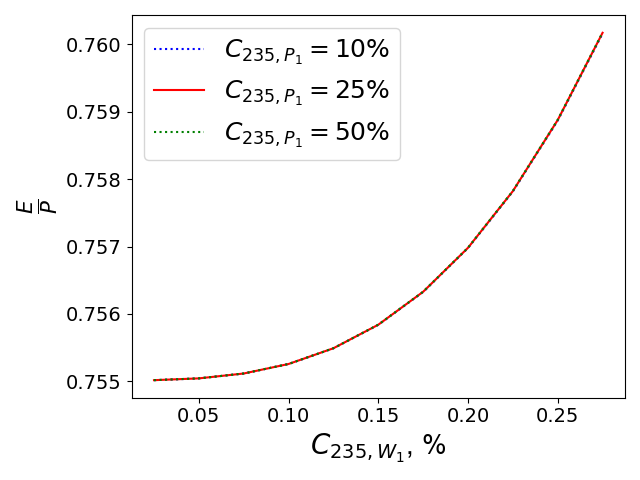
\includegraphics[scale=0.5]{images/2023/Figure_6}}
  \caption{Расход регенерата на единицу конечного НОУ-продукта для различных  $C_{235, P_1}$ и $C_{235, W_1}$ каскада, обогащающего регенерат (кривые зависимостей совпадают)}\label{Figure_10}
\end{figure}

% , для которого удельный расход природного урана составляет $\approx$7,93 (см. Приложение).

% \begin{figure}[ht]
%   \centerfloat{\includegraphics[scale=0.5]{images/plots/sc2_LEU_D}}
%   \caption{Концентрация $^{235}$U в разбавителе, необходимая для получения свежего НОУ для различных концентраций $^{235}$U в потоках продукта и отвала каскада, обогащающего регенерат}\label{fig:sc2_LEU_D}
% \end{figure}

% Проиллюстрировать затраты на работу разделения от составных  частей каскадной схемы, можно с помощью рис.\ref{myplot}, который показывает, что доля центрифуг для приготовления разбавителя из природного урана выше, чем доля центрифуг, задействованных для предварительного обогащения регенерата, и эта пропорция уменьшается с понижением содержания $^{235}$U в $W_0$.

% \begin{figure}[ht]
%   \centerfloat{\includegraphics[scale=0.5]{images/plots/myplot}}
%   \caption{Отношение количества центрифуг в каскаде, производящем разбавитель из природного урана, к количеству центрифуг, задействованных для предварительного обогащения регенерата, для различных концентраций $^{235}$U в потоках продукта и отвала каскада, обогащающего регенерат}\label{myplot}
% \end{figure}

Рисунок \ref{fig3__7} иллюстрирует изменение концентрации $^{235}$U в разбавителе $(F_n)$ для различных концентраций этого же изотопа в потоках $P_1$ и $W$. Для каждой из точки на графиков удалось выполнить все ограничения на концентрации четных изотопов в товарном НОУ. Как видно, несмотря на возможность варьирования концентрации $^{235}$U в разбавителе, допустимый диапазон оказывается фактически узким (от 4,1 до 4,6\%). Данное обстоятельство можно объяснить тем, что при смешивании разбавителя и обогащенного регенерата основная доля по массе приходится на разбавитель. Это означает, что концентрация в нем не может заметно отличаться от требуемой концентрации $^{235}$U в конечном продукте.   

\begin{figure}[ht]
  \centerfloat{\includegraphics[scale=0.5]{images/2023/Figure_7}}
  \caption{Концентрация $^{235}$U в НОУ-разбавителе $F_n$ для различных $C_{235, P_1}$ и $C_{235, W_1}$ каскада, обогащающего регенерат}\label{fig3__7}
\end{figure}

Подытоживая анализ результатов вычислительных экспериментов для данной модификации ординарного каскада, можно заключить, что она непригодна для решения задачи обогащения в условиях многократного рецикла, так как с ее помощью нет возможности использовать весь регенерированный уран на производство НОУ-продукта (рис. \ref{Figure_10}). Тем не менее, рассмотренная каскадная схема может быть использована для решения задачи повторного использования урана для возврата (дообогащения) регенерата с относительно низким исходным содержанием четных изотопов, что соответствует первому рециклу или низкой глубине выгорания топлива \cite{smirnovKaskadnyeShemyZadachah2012}.

\subsection{Анализ схемы с разбавлением предварительно обогащенного природного урана регенератом}\label{sw_method}

Проанализируем возможность решения задачи обогащения регенерированного урана со всеми ограничениями в каскадной схеме с разбавлением предварительно обогащенного природного урана регенератом (рис. \ref{o2}). Принцип работы такой схемы состоит в том, что предварительно обогащенный природный уран смешивается с возвращаемым в топливный цикл регенерированным ураном. Уровень предварительного обогащения (перед смешением) природного урана и отношение потоков обогащенного природного урана к регенерату определяются исходя из условий задачи. Таким образом, данная схема в принципе аналогична схеме рисунка \ref{o1}. Это означает, что ей присущ тот же принципиальный недостаток, что и упомянутой схеме, а именно: число ее управляющих параметров меньше, чем число условий, требующих одновременного выполнения. 

\begin{figure}[ht]
  \centerfloat{\includegraphics[scale=0.035]{cascades/ord2}}
  \caption{Схема каскада с разбавлением предварительно обогащенного природного урана регенератом. Обозначения: $E$ --- регенерат, $F_n$ --- природный уран; $W_1$ --- поток отвального ОГФУ тяжелого конца каскада; $P$ --- поток товарного низкообогащенного урана}\label{o2}
\end{figure}

Для ответа на вопрос о возможности использования данной схемы для обогащения регенерата в условиях многократного рецикла были проведены вычислительные эксперименты, в рамках которых варьировали величину концентрации $^{235}$U в обогащенном природном уране и отношение, в котором смешиваются разбавитель с регенератом с целью найти такой набор параметров схемы, при которых сформулированная в разделе \ref{ch2_stat} задача будет решена. Как и в рассмотренных выше примерах моделирование процесса обогащения урана в каскаде осуществляли с использованием $R$-каскада. Концентрацию $^{235}$U в отвале каскада задавали равной 0,1\%.

Ниже приведены результаты расчета параметров схемы с разбавлением предварительно обогащенного природного урана регенератом при решении задачи обогащения регенерата с учетом сформулированных выше условий.
\begin{table}[ht]
  \centering
  \caption{Параметры схемы с разбавлением предварительно обогащенного природного урана регенератом (рис. \ref{o2}).}\label{MDKparams}
    \normalsize\begin{tabulary}{1.0\textwidth}{|c|c||c|c||c|c|}
      \hline $\frac{F_n}{P}$ & $\delta(\frac{F_n}{P}), \%$ & $\frac{\Delta A}{P}, \textit{{\tiny ЕРР}}$ & $\delta(\frac{\Delta A}{P}), \%$ & $\frac{E}{P}$ \\
      \hline $6,647$ & $13,58$ & $12,03$ & $-1,86$ & $0,755$ \\\hline
  \end{tabulary}
\end{table}
% \begin{table}[ht]
%   \centering
%   \caption{Концентрации изотопов в товарном НОУ (поток $P$) и выходящих потоках каскада I (поток $P_{1}$, $W_{1}$) (рис. \ref{o2})}\label{casORDch3params} 
%   \begin{tabular}{|c|c|c|c|c|}
%       \hline Массовое число & $C_{i}^{P_{1}}, \%$ & $C_{i}^{W_{1}}, \%$ & $C_{i}^{P}, \%$\\
%       \hline 232 & --- & --- & $5,0\cdot10^{-7}$ \\
%       233 & --- & --- & $1,41\cdot10^{-6}$ \\
%       234 & $0,14$ & $2,1\cdot10^{-4}$ & $5,93\cdot10^{-2}$ \\
%       235 & $16,72$ & $0,1$ & $5,17$ \\
%       236 & --- & --- & 0,75 \\
%       238 & Остальное & Остальное & Остальное \\
%       \hline
% \end{tabular}
% \end{table}

В таблице \ref{MDKparams} приведены интегральные параметры рассматриваемой схемы: удельные величины затрат работы разделения $\frac{\Delta A}{P}$ и расхода природного урана $\frac{F_n}{P}$, а также их относительное изменение по сравнению с аналогичными характеристиками ординарного каскада для обогащения природного урана в открытом топливном цикле с теми же внешними условиями. Величина $\frac{\Delta A}{P}$ для рассматриваемых каскадных схем приводится в единицах работы разделения (ЕРР).
% и оценена, как отношение суммарного потока рассматриваемого каскада для обогащения регенерата к суммарному потоку ординарного каскада для обогащения природного урана при тех же внешних условиях, умноженное на величину работы разделения, рассчитанную для последнего по известной формуле:
Следует отметить, что понятия «работа разделения» и «единица работы разделения» (ЕРР) изначально введены для двухкомпонентных смесей. Для многокомпонентной смеси и, в том числе, смеси регенерированного урана, устоявшийся и общепринятый аналог понятию «работа разделения» отсутствует \cite{2024sep_potential_ifz}. Поэтому в приведенных ниже результатах под работой разделения подразумевали условную величину, прямо пропорциональную суммарному потоку каскада. В случае идентичности разделительных элементов (газовых центрифуг) в каскаде и эквивалентности режимов их работы эта величина будет также прямо пропорциональна числу газовых центрифуг в каскаде, что можно в целом записать как:

\begin{equation}\label{AvsP_2024}
  \frac{A}{P}=a\sum_{s=1}^N L_s=b\sum_{s=1}^N Z_s \, ,\quad a,b>0 \; ,
\end{equation}
где $L_s$ -- поток питания ступени каскада с номером $s$, $Z_s$ --  число разделительных элементов в ступени с номером $s$, $a$ и $b$ -- коэффициенты пропорциональности. Коэффициенты $a$ и $b$ в формуле \ref{AvsP_2024} определяются параметрами одиночного разделительного аппарата и свойствами разделяемой смеси, и в общем случае будут отличаться для смесей природного и регенерированного урана. Однако, предположив, что величины $a$ и $b$  остаются одинаковыми для обеих смесей, можно записать условие:

\begin{equation}\label{AvsP_regnat_2024}
  \frac{(A/P)_{reg}}{(A/P)_{nat}} \approx \frac{(\sum_{s=1}^N L_s)_{reg}}{(\sum_{s=1}^N L_s)_{nat}} \; ,
\end{equation}
где $(A/P)_{reg}$ -- дельная работа разделения при обогащении регенерата урана,  $(A/P)_{nat}$ -- удельная работа разделения при обогащении природного урана.

Предположение об одинаковости коэффициентов $a$ и $b$ для смесей природного урана и регенерированного урана означает, что величина разделительной способности одиночного аппарата остается одинаковой в обоих случаях. Условие \ref{AvsP_regnat_2024} позволяет сделать оценку величины работы разделения в ЕРР при обогащении регенерированного урана, которая имеет смысл только для использования в практических оценочных расчетах, например, в рамках технико-экономических исследований различных вариантов реализации ЯТЦ. Для этого из \ref{AvsP_regnat_2024} можно получить:

\begin{equation}\label{AvsP_reg_2024}
  (A/P)_{reg}=\frac{(\sum_{s=1}^N L_s)_{reg}}{(\sum_{s=1}^N L_s)_{nat}} \cdot (A/P)_{nat} \; .
\end{equation}

Учитывая, что расчеты параметров каскада осуществляли с использованием модели R-каскада, которая в случае разделения бинарной смеси природного урана совпадает с предложенной К. Коэном моделью идеального каскада, величину $(A/P)_{nat}$ можно рассчитать по известной формуле:

\begin{equation}\label{kohen_2024}
  \begin{gathered}
    (A/P)_{nat}=\left(2 \cdot C_p-1\right) \cdot \ln \frac{C_P}{1-C_P}+\frac{C_P-C_F}{C_F-C_W} \cdot \\
    \cdot \left(2 \cdot C_W-1\right) \cdot \ln \frac{C_W}{1-C_W}-\frac{C_P-C_W}{C_F-C_W} \cdot \left(2 \cdot C_F-1\right) \cdot \ln \frac{C_F}{1-C_F} \; .
  \end{gathered}
\end{equation}

Важно подчеркнуть, что формула \ref{AvsP_reg_2024} не имеет под собой строгого физического обоснования и может  применяться только для оценочных расчетов, а рассчитанная с ее использованием величина условной работы разделения носит лишь справочный характер.

% \begin{equation}\label{SWU_Phi}
%   (\frac{\Delta A}{P})_{\textit{ord.}}=\Phi\left(C_P, C_F, C_W\right),
%   \end{equation}
% где $\Phi$, называемая функцией ценности, представляет собой удельную работу разделения \cite{cohenTheoryIsotopeSeparation1951,sulaberidzeTeoriyaKaskadovDlya2011}:
% \begin{equation}\label{Phi}
%   \begin{gathered}
%     \Phi\left(C_P, C_F, C_W\right)=\left(2 \cdot C_p-1\right) \cdot \ln \frac{C_P}{1-C_P}+\frac{C_P-C_F}{C_F-C_W} \cdot \\
%     \cdot \left(2 \cdot C_W-1\right) \cdot \ln \frac{C_W}{1-C_W}-\frac{C_P-C_W}{C_F-C_W} \cdot \left(2 \cdot C_F-1\right) \cdot \ln \frac{C_F}{1-C_F} \; .
%   \end{gathered}
% \end{equation}
  
% Работа разделения для каскада, обогащающего регенерат в этом случае рассчитана по формуле:

% \begin{equation}\label{SWU_cas}
%   \frac{\Delta A}{P}=\frac{\sum_{s=1}^N L_s}{(\sum_{s=1}^N L_s)_{\textit{ord.}}}\cdot (\frac{\Delta A}{P})_{\textit{ord.}} \; .
% \end{equation}

Такая методика оценки величин работы разделения будет и далее, использована в диссертации при расчете величины работы разделения для каскадных схем обогащения регенерата.

Для всех рассмотренных ниже каскадных схем помимо абсолютных значений затрат работы разделения и расхода природного урана рассчитывали также их относительные изменения по отношению к значениям $(\frac{\Delta A}{P})_{ord.}$ и $(\frac{F_n}{P})_{ord.}$, соответствующим ординарному каскаду для обогащения природного урана, в котором нарабатывают товарный НОУ при тех же внешних условиях. Далее будем называть такую каскадную схему референтной, и приведем основные параметры, рассчитанные с использованием модели $R$-каскада  (таблица \ref{ordninary495}). Здесь и далее, для всех случаев, кроме тех, что специально будут оговорены, относительные изменения величин $\frac{\Delta A}{P}$ и $\frac{F_n}{P}$ рассчитаны по отношению к приведенным в таблице \ref{ordninary495} значениям (Подробнее в Приложении А).

\begin{table}[ht]
    \centering
    \caption{Параметры ординарного каскада для обогащения природного урана (рис. \ref{uranfN}) до 4,95\% с 0,1\% в отвале при $q_0=\sqrt[3]{1,2}$, $M^{*}$=236,5.}\label{ordninary495}
    \normalsize\begin{tabulary}{1.0\textwidth}{|c|c|c|c|c|c|}
        \hline $\frac{F}{P}$ & $\frac{P}{F}$ & $\frac{W}{F}$ & $f$ & $N$ & $\frac{\Delta A}{P}, \textit{{\tiny ЕРР}}$\\
        \hline $7,93$ & $0,126$ & $0,874$ & 21,59 & 42,35 & 11,82\\\hline
    \end{tabulary}
\end{table}

Относительные значения изменения величин работы разделения и расхода природного урана рассчитывали по формулам:

\begin{equation} \label{DeltaA} 
  \delta(\frac{\Delta A}{P})=1-\frac{\Delta A}{P}/(\frac{\Delta A}{P})_{ord.} \; ,
\end{equation}
где $(\frac{\Delta A}{P})_{ord.}$ --- удельная величина работы разделения для ординарного каскада, обогащающего природный уран в открытом топливном цикле при идентичных внешних условиях (таблица \ref{ordninary495}), а величина $\frac{\Delta A}{P}$ пропорциональна суммарного потоку каскада с разбавлением предварительно обогащенного природного урана регенератом.

\begin{equation} \label{DeltaFnu} 
  \delta(\frac{F_n}{P})=1-\frac{F_n}{P}/(\frac{F_n}{P})_{ord.} \; ,
\end{equation} 
где $(\frac{F_n}{P})_{ord.}$ --- величина удельного расхода природного урана для референтного ординарного каскада (таблица \ref{ordninary495}), вычисляемая с помощью уравнения \ref{GrindEQ__1_70_}.

Положительная величина $\delta(\frac{\Delta A}{P})$ соответствует достигаемой экономии работы разделения относительно референтной схемы (ординарного каскада для обогащения природного урана), а отрицательная --- перерасходу работы разделения. Положительная величина $\delta(\frac{F_n}{P})$ соответствует экономии природного урана относительно референтной схемы (ординарного каскада для обогащения природного урана), а отрицательная --- его относительному перерасходу.


Из результатов вычислительных экспериментов следует, что для рассматриваемой схемы возможно получение решения, удовлетворяющего заданным ограничениям на концентрации изотопов $^{232,234,236}$U. Однако, как и в случае применения схемы рис. \ref{o1}, одновременно с этими условиями не удается удовлетворить условие возврата заданной массы регенерата. В результате вместо заданной величины отношения массы исходного регенерата к продукту --- 0,93, фактические значения не превысили величины 0,755. Данные результаты свидетельствуют о том, что такая схема обогащения регенерата не решает поставленную задачу для произвольного изотопного состава регенерата и, следовательно, не может быть применена в условиях многократного рецикла урана в топливе легководных реакторов.


\subsection{Анализ схемы с разбавлением регенерата природным ураном перед подачей в ординарный трехпоточный каскад}

Еще одним вариантом каскадной схемы для обогащения регенерированного урана, основанной на использовании ординарного каскада является схема, в которой смешивание и разбавление регенерата происходит непосредственно перед подачей в каскад для последующего обогащения (рис. \ref{o3}). В качестве разбавителя здесь, как правило, рассматривают природный уран. Соотношение, в котором следует смешать природный и регенерированный уран определяют, исходя из ограничений на концентрации четных изотопов в конечном НОУ-продукте.

\begin{figure}[ht]
  \centerfloat{\includegraphics[scale=0.035]{cascades/ord3}}
  \caption{Схема каскада со смешением регенерата и природного урана перед подачей на питание ординарного каскада. Обозначения: $E$ --- поток питающего схему регенерата, $F_n$ --- поток разбавителя; $W_1$ --- поток отвального ОГФУ тяжелого конца каскада; $P$ --- поток товарного низкообогащенного урана}\label{o3}
\end{figure}

В случае, если разбавитель известен, то для такой схемы существует единственный управляющий параметр --- это отношение, в котором смешиваются потоки регенерата и природного урана. Очевидно, что с ростом доли регенерата в совокупном питании каскада (смесь потоков $E$ и $F_n$) будут возрастать концентрации четных изотопов в потоке отбора каскада. Это обуславливает тот факт, что существует некоторое критическое значение этого отношения, начиная с которого уже невозможно будет соблюсти, как минимум, ограничение на концентрацию изотопа $^{232}$U. Для рассматриваемой схемы проведены вычислительные эксперименты, в которых варьировали отношение разбавления между регенератом и разбавителем, в качестве которого рассматривали уран природного состава. Кроме того, в диапазоне 0,05--0,3\% варьировали концентрацию изотопа $^{235}$U в потоке отвала каскада $W_1$. Как и во всех рассмотренных в рамках данной главы примерах исходные условия соответствовали задаче, описанной в разделе \ref{ch2_stat}, а в качестве расчетной модели использован $R$-каскад. Расчеты проведены на примере состава 1 таблицы \ref{is_compositions_2_5}. 

На рис. \ref{sc3_1.second} отражена взаимозависимость отношения потоков $E/P$ и концентрации $^{232}$U в конечном продукте. Зависимости построены при различных $C_{235, W_1}$. Как следует из анализа представленных зависимостей, во всех случаях величина концентрации  $^{232}$U достигает предельного значения ($5\cdot10^{-7}$\%) ранее, чем отношение между исходным регенератом и продуктом достигнет требуемого значения --- 0,93. Это означает, что и эта схема также не позволяет решить полностью задачу обогащения регенерата с относительно высоким содержанием четных изотопов. Иными словами схема также оказывается непригодной к обогащению регенерированного урана в условиях многократного рецикла.

\begin{figure}[ht]
  \centerfloat{\includegraphics[scale=0.5]{images/2023/3_11}}
  \caption{Расход регенерированного урана на единицу НОУ-продукта при различной концентрации $^{232}$U в питающем потоке каскада для различных концентраций $^{232}$U в потоке НОУ-продукта $P$}\label{sc3_1.second}
\end{figure}

% \begin{figure}[ht]
%   \centerfloat{\includegraphics[scale=0.5]{images/plots/3.11new}}
%   \caption{Расход регенерированного урана на единицу НОУ-продукта  при различной концентрации $^{232}$U в питающем потоке каскада для различных концентраций $^{235}$U в потоке отвала. Обозначения: см. - смесь природного урана и регенерата, подаваемая на питание каскада}\label{sc3_1.second}
% \end{figure}

\subsection{Аналитический подход к оценке возможности использования модификаций ординарного каскада для обогащения регенерированного урана в условиях многократного рецикла}

Описанные выше результаты вычислительных экспериментов, показали не применимость схем на основе ординарного каскада в условиях  многократного рецикла. Это обусловлено ухудшением изотопного состава урана по мере прохождения им серии топливных циклов (накопление $^{232}$U и других четных изотопов). При этом исходная концентрация $^{232}$U питающей смеси, начиная со второго рецикла, превышает уровень допустимый в конечном продукте, поэтому схемы, основанные на ординарном каскаде, которые только <<разбавляют>> этот изотоп, не эффективны для решения поставленной задачи. Тем не менее, если рассматривать подобные схемы для обогащения регенерированного урана, прошедшего только однократное облучение или допустить <<послабление>> ограничений на концентрации четных изотопов, то подобные схемы, безусловно, могут быть применены для решения задачи обогащения регенерированного урана.

При этом закономерно возникает следующий вопрос: возможно ли априорно оценить возможность решить поставленную в (\ref{ch2_stat}) задачу в таких модификациях ординарного каскада? 

На этот вопрос можно ответить, обратившись к уравнениям баланса компонентов в каскаде (\ref{GrindEQ__1_21_}) по крайней мере в случае вариантов каскадных схем, где регенерированный уран поступает в каскад для обогащения. Запишем уравнение материального баланса для изотопа $^{232}$U, учитывая, его малую концентрации в исходной смеси, в предположении, что его концентрация в отвале каскада будет стремиться к нулю. Данное предположение может быть вполне оправдано, если отвальная часть каскада имеет достаточное число ступеней. В этом случае $^{232}$U, являясь самым легким в смеси регенерированного урана, будет активнее остальных компонентов концентрироваться в отборе каскада. Это означает, что для изотопа $^{232}$U уравнение материального баланса можно переписать в следующем виде, пренебрегая слагаемым с потоком отвала каскада:

\begin{subequations}\label{mat_balance12}
  \begin{empheq}[left=\empheqlbrace]{align}
    &F_n+E=P+W, \\
    &F_n \cdot C_{232,F_n} + E \cdot C_{232,E} = P \cdot C_{232,P} + W \cdot C_{232,W} \; .
  \end{empheq}
\end{subequations}

Учитывая условия:

\begin{equation} \label{mat_balance3} 
  C_{232,F_n}=0 ,\; C_{232,W} \rightarrow 0 \; ,
\end{equation} 
можно оценить верхнюю границу для концентрации $^{232}$U в потоке $P$ для заданного значения $\frac{E}{P}$: 
% \begin{equation}
% \label{eq_232_balance}
%   C_{232,P} \approx \frac{RepU}{P} C_{232,RepU}
% \end{equation}

\begin{equation}
  \label{eq_232_balance_}
    C_{232,P} \approx \frac{E}{P} \cdot C_{232,E} \; ,
\end{equation}
откуда при заданной предельной концентрации $^{232}$ в товарном НОУ легко получить оценку для максимальной концентрации этого изотопа в поступающем на обогащение регенерате: 

\begin{equation}
  \label{eq_232_balance_var2}
    C_{232,E} \approx \frac{P}{E} \cdot {{(}{C_{232,P}}{)}}_{lim} \; ,
  \end{equation}
где ${{(}{C_{232,P}}{)}}_{lim}$ --- предельная концентрация $^{232}$U в товарном НОУ.
  
Учитывая, что величина $\frac{E}{P}$ в приведенном выше уравнении и является отношением (исходный регенерат)/продукт, условие $\frac{E}{P}\approx$0,9-0,95 будет выполнено только, если концентрация $C_{232,E}$ составляет не более $\approx$1,05-1,1 от величины ${{(}{C_{232,P}}{)}}_{lim}$. Это позволяет оценить максимальную величину $C_{232,E}$, при которой еще будет возможно решить задачу обогащения регенерата. Например, для $\frac{E}{P}=0,93$ и $C_{232,P}=5\cdot10^{-7}\%$ получаем величину $\approx 5,37\cdot10^{-7}\%$, что оказывается меньше, чем в составах 1 и 2 таблицы \ref{is_compositions_2_5}. С другой стороны, зная $C_{232,E}$, с помощью уравнения (\ref{eq_232_balance_}) можно вычислить максимально возможную долю питающего потока, содержащего $^{232}$U, как неизвестную переменную уравнения (\ref{eq_232_balance_}). Например, для состава 1 таблицы \ref{is_compositions_2_5}, который был использован в рассмотренных выше примерах получаем:

% \begin{equation}
%   \label{eq_232_balance_X}
%     5 \times 10^{-7} \% \approx X \times 6.622 \times 10^{-7} \% \Rightarrow X \approx 0.755
% \end{equation}

\begin{equation}
  \label{eq_232_balance_X_}
    \frac{E}{P} \leq 0,755 \; .
\end{equation}

Снова анализируя представленные в предыдущих разделах данные, легко увидеть, что полученные в результате прямого численного расчета предельные величины отношений (исходный регенерат)/продукт приблизительно и составляют такую величину.

Важно сделать акцент на том, что при фактическом $\frac{E}{P}\leq 0,755$ вместо требуемых в рассматриваемом примере $\frac{E}{P}=0,93$, возникает некоторая масса регенерированного урана, которая не участвует в процессе возврата урана в топливный цикл, тем самым означая вывод из оборота части массы $^{235}$U (в данном случае: $0,93-0,755=0,175$ или 17,5\%). Далее, частичная потеря изотопа $^{235}$U происходит непосредственно при его обогащении в каскаде из-за наличия потока отвала. Задавая степень извлечения изотопа $^{235}$U в каскаде в диапазоне 75-85\%, общие потери целевого изотопа $^{235}$U в топливном цикле при использовании такой каскадной схемы могут составит 30-38\% от исходной массы $^{235}$U в поступившем в обогащение регенерате.

% Описанный выше подход позволяет аналитически оценить возможность применения схем на основе простейших модификаций ординарного каскада, исходя из изотопного состава регенерата.
Следует отметить, что подобные оценки можно также применять и для каскадных схем, в которых регенерат разбавляют уже внутри каскада, путем его подачи в качестве дополнительного питания, поскольку такие схемы по сути являются также только разбавляющими, а балансные соотношения для них будут выглядеть аналогично (\ref{mat_balance12}).

\subsection{Общие выводы о возможностях схем возврата регенерата в ЯТЦ на основе ординарного каскада}

Обобщая описанные выше результаты вычислительных экспериментов, проведенных для различных модификаций ординарного каскада для обогащения и разбавления регенерированного урана, можно сделать следующие основные выводы:
\begin{enumerate}
  \item Представленные на рисунке \ref{fig:diagram1ch3} варианты каскадных схем принципиально не решают задачу обогащения регенерированного урана при одновременном выполнении условий на концентрации четных изотопов в товарном НОУ и обеспечения расходования заданной массы регенерата на получение этого НОУ для составов регенерата с исходным высоким содержанием четных изотопов (например, для концентраций $^{232}$U, исходно превышающих предельные значения для товарного НОУ). 
  \item Основная причина невозможности решения задачи состоит в том, что в рассматриваемых схемах число свободных параметров оказывается меньшим, чем число условий, которые необходимо одновременно удовлетворить. В результате такие схемы могут обеспечить решение задачи только в некоторых частных случаях, например, когда в обогащение поступает регенерированный уран с концентрациями четных изотопов, в первую очередь, $^{232}$U ниже, чем предельные значения для товарного НОУ. Поэтому такие схемы возможно эффективно использовать только обогащения однократно облученного уранового топлива --- так называемый регенерат первого рецикла. 
  \item Полученные результаты однозначно свидетельствует о том, что для обогащения регенерированного урана в условиях многократного рецикла необходимо использование более сложных вариантов каскадных схем, которые смогут позволить полностью решить поставленную задачу обогащения регенерата безотносительно к его исходному составу и другим внешним условиям.
\end{enumerate}

\section{Обоснование необходимости составных схем}

Как следует из описанных выше результатов, на текущий момент в принципе имеются способы, позволяющие обеспечить выполнение требований по четным изотопам урана при обогащении регенерата. Однако основной проблемой, решаемой в рамках настоящей работы, является поиск варианта каскадной схемы, позволяющей одновременно выполнить ограничения по концентрациям четных изотопов и задействовать в обогащении весь имеющийся регенерат в условиях неопределенности его изотопного состава при многократном рецикле.

Если анализировать причины невозможности возврата массы регенерата в производство топлива в различных модификациях ординарного каскада для обогащения регенерата в условиях многократного рецикла, то становится очевидным, что это, во многом, связано с нарастанием относительных концентраций <<легких>> изотопов (в первую очередь $^{232}$U) и $^{235}$U. Поскольку данные изотопы концентрируются вместе на легком <<конце>> каскада, то единственным способом понизить отношение их концентраций --- это разбавить материалом, не содержащим $^{232}$U, $^{236}$U. Как показали результаты, описанных в этой главе вычислительных экспериментов, для составов с относительно высоким исходным содержанием $^{232}$U невозможно подобрать такой разбавитель, чтобы удовлетворить одновременно и условие полного возврата массы регенерата в цикл и ограничения на содержание четных изотопов.

Из приведенного выше анализа следует, что эффективная каскадная схема для обогащения регенерата урана при многократном рецикле должна обеспечивать не только разбавление регенерата, но и частично его очистку от четных изотопов. Поэтому возможные варианты решения задачи, по-видимому, должны быть основаны на использовании схем двойных каскадов, в том числе, описанных в Главе \ref{ch1}. В связи с этим представляет интерес оценка возможности прямого обогащения регенерата с повышенным содержанием четных изотопов в двойном каскаде с целью решения задачи обогащения регенерата в наиболее общей постановке. Этот вопрос и рассмотрен в следующих разделах настоящей главы.

\section{Двойной каскад}\label{sec:ch2/dvoynoy}

Двойной каскад для обогащения регенерата рассмотрен в литературном обзоре (см. \ref{ch1/dvoynoy}) и представляет собой последовательное соединение двух каскадов (рис. \ref{fig:double_ru_in3}). 

\begin{figure}[ht]
  \centerfloat{\includegraphics[scale=0.07]{cascades/Double_core}}
  \caption{Двойной каскад. Обозначения: $E$ --- поток питающего схему регенерата, $W_1$ --- поток отвального ОГФУ тяжелого конца каскада; $P$ ($W_2$) --- конечный НОУ продукт на основе регенерата; $P_2$ --- отход двойного каскада в виде высокообогащенного урана; $F_0$ --- природный уран; $P_0$ --- дополнительно производимый НОУ продукт для возможности загрузить активную зону реактора}\label{fig:double_ru_in3}
\end{figure}

Напомним кратко суть работы этой схемы. Двойной каскад позволяет сконцентрировать нежелательные четные изотопы отдельно от изотопа $^{235}$U. Для этого сначала в каскаде I обогащают изотоп $^{235}$U с одновременным обогащением изотопов $^{232}$U, $^{234}$U, $^{236}$U, а затем полученную смесь направляют на вход каскада II (рис. \ref{fig:double_ru_in3}), где она делится на две группы: в первой обогащены легкие изотопы ($^{232}$U, $^{234}$U и $^{235}$U), во второй обедняется $^{235}$U с более интенсивным обеднением $^{232}$U, $^{234}$U. Это позволяет в потоке $W_2$ получить низкообогащенный уран, отвечающий требованиям по концентрациям изотопов $^{232}$U, $^{234}$U с одновременной компенсацией $^{236}$U.

Нужно учитывать, что для двойного каскада выполнено очевидное условие $E>W_2$, а чаще всего $E \gg W_2$. Это означает, что при рассмотрении в рамках топливного цикла, подразумевающем необходимость обеспечения реактора ядерным топливом, такой каскад может произвести лишь небольшую часть топлива для загрузки реактора. Остальную массу необходимо получить другим путем, например, обогащением природного урана. Это иллюстрирует третий каскад на рис. \ref{fig:double_ru_in3}, который нарабатывает из природного урана (поток $F_0$) недостающую массу ядерного топлива для загрузки реактора. В этом контексте интерес представляет оценка эффективности такой каскадной схемы в топливном цикле при условии обогащения регенерированного урана с относительно высоким содержанием четных изотопов. Для этого в рамках работы проведены вычислительные эксперименты, направленные на получение ответа на эти вопросы. В качестве модели для описания процессов селективного массопереноса в каждом из каскадов схемы использован $R$-каскад. 

При этом рассматривали разделительную задачу в следующей постановке.

Задано:

\begin{itemize}
    \item концентрации компонентов в обогащаемом регенерированном уране: $C_{i,{E}}$; 
    \item величина концентрации $^{235}$U в потоке $W_{1}$: $C_{235,{W_1}}$;
    \item параметры одиночного разделительного элемента (центрифуги): величины потока питания центрифуги ($l_{ГЦ}$) и коэффициента разделения, приходящегося на единичную разность массовых чисел ($q_{0}$);
    \item величина потока $E$ (определяется массой поступившего в обогащение регенерата);
    \item в случае использования $R$-каскада необходимо задание пары компонентов, по которым должно быть выполнено условие несмешивания их относительных концентраций (подробнее см. Главу \ref{ch2_theory}).
\end{itemize}

Параметры каскадной схемы, соответствующие требованиям, предъявляемым к получаемому товарному НОУ:

\begin{itemize}
    \item величина концентрации $^{235}$U в продукте (товарном НОУ, поток $P$ ($P \equiv W_2$) на схеме рис. \ref{p2left}): $C_{235,{P}}$;
    \item величины предельных концентраций изотопов $^{232}$U и $^{234}$U в конечном продукте $P$: $(C_{232,{P}})_{lim}$;
    \item величины предельно допустимого отношения концентраций изотопа $^{234}$U и $^{235}$U в конечном продукте $P$: ${C_{234,{P}}}/{C_{235,{P}}}$;
    \item величина концентрации $^{235}$U в потоке отвала каскада I: $C_{235,{W_1}}$;
    \item вид функции $f(C_{236,P})$, в соответствии с которой рассчитывают конечную (эквивалентную) величину обогащения по $^{235}$U в продукте, с учетом компенсации присутствия $^{236}$U:
    $(C_{235,P})_\textit{экв.}=(C_{235,P})_\textit{прир.}+f(C_{236,P})$.    
\end{itemize}

Расчет параметров рассматриваемой каскадной схемы строится на основе результатов последовательного расчета каждого из каскадов схемы. Причем для отдельных каскадов осуществляют проектировочный расчет их параметров (см. Главу \ref{ch2_theory}), когда в качестве заданных величин выступают концентрации одного из компонентов смеси в потоках отбора и отвала каскада, а искомыми параметрами выступают полное число ступеней в каскаде и номер ступени подачи внешнего питания для $R$-каскада. Таким образом, для каждого из каскадов при заданных концентрациях компонентов в потоках питания, величине одного из внешних потоков ($F$, $P$ или $W$), параметрах одиночного разделительного элемента, для расчета их остальных параметров необходимо задать еще 2 величины. Такой парой параметров как раз и могут выступать концентрации целевого компонента в потоках отбора и отвала каскада. Задание этих величин позволяет, используя уравнения (\ref{GrindEQ__1_72_}), (\ref{GrindEQ__1_73_}), определить неизвестные величины $N$ и $f$ для каждого из каскада и далее по соотношениям (\ref{GrindEQ__1_70_})-(\ref{GrindEQ__1_77_}) рассчитать все их внешние и внутренние параметры. Тем самым имеем ситуацию, при которой для последовательного расчета параметров каждого из каскадов схемы, учитывая, что величина $C_{235,{W_1}}$ задана по условию, необходимо задать еще 3 величины: $C_{235,{P_1}}$, $C_{235,{P_2}}$ и $C_{235,{P}}\equiv C_{235,{W_2}}$. Причем концентрация $C_{235,{P}}$ также попадает в эту группу, поскольку точное определение данной величины возможно только, если известна конечная концентрация $^{236}$U в НОУ, которую нужно скомпенсировать. Таким образом, неизвестными переменными задачи будут величины $C_{235,{P_1}}$, $C_{235,{P_2}}$ и $C_{235,{P}}$, определяющие полные числа ступеней и номера ступеней подачи питаний в каскадах I и II.

Для нахождения 3-x неизвестных, имеем 2 независимых уравнения:  

\begin{equation}
    \label{dis_235_6_ch3}
    \Delta_{236}=(C_{235,P})_{\textit{экв.}}-((C_{235,P})_n+\Delta C_{235}),
\end{equation}
где $\Delta_{236}$ --- невязка по концентрации $^{235}$U в конечном НОУ-продукте, с учетом поправки на присутствие изотопа $^{236}$U. $(C_{235,P})_{\textit{экв.}}$ --- эквивалентная концентрация $^{235}$U в потоке товарного НОУ, $(C_{235,P})_n$ --- требуемая концентрация $^{235}$U в товарном НОУ без учета компенсации влияния $^{236}$U, $\Delta C_{235}$ --- величина добавочного обогащения изотопа $^{235}$U для компенсации влияния $^{236}$U. 

\begin{equation}
\label{dis_232_ch3}
\Delta_{232}=\left|C_{232,P\textit{calc}}-C_{232,P\textit{given}}\right|,
\end{equation}
где $\Delta_{232}$ --- разница (по абсолютной величине) между рассчитанным значением концентрации $^{232}$U в конечном НОУ-продукте ($C_{232,P\textit{calc}}$) и заданной предельной величиной для концентрации этого изотопа ($C_{232,P\textit{given}}$).

Величины $\Delta_{232}$ и $\Delta_{236}$ определяют выполнение условия компенсации $^{236}$U при достижении требуемого в НОУ-продукте обогащения по $^{235}$U и требования к максимально допустимой концентрации изотопа $^{232}$U в продукте. Отметим, что условие (\ref{dis_232_ch3}) представляет собой частный случай более общего условия $C_{232,P\textit{calc}}-C_{232,P\textit{given}}\leq 0$, которое более корректно отражает суть требования о непревышении концентрацией $^{232}$U заданного предела. Однако для решения задачи более удобно строго задать ограничение в виде равенства. 

Уравнения системы (\ref{dis_235_6_ch3})-(\ref{dis_232_ch3}) отражают неявные зависимости величин концентраций изотопов $^{232}$U и $^{235}$U в потоке $P$ (или $W_2$) от искомых концентраций $C_{235,{W_2}}$, $C_{235,{P_1}}$, $C_{235,{P_2}}$. Это означает, что возможно только численное решение системы уравнений (\ref{dis_235_6_ch3})-(\ref{dis_232_ch3}) с расчетом параметров каскадов I и II на каждой итерации процедуры решения. Причем для расчета параметров каскадов I-II для каждой итерации решения системы (\ref{dis_235_6_ch3})-(\ref{dis_232_ch3}) необходимо отдельно численно решать системы уравнений вида (\ref{dis_235P})-(\ref{dis_235W}) для каждого из каскадов схемы. Решение систем уравнений (\ref{dis_235_6_ch3})-(\ref{dis_232_ch3}) и (\ref{dis_235_6_ch3})-(\ref{dis_232_ch3}) возможно осуществить одним из известных численных методов решения систем нелинейных уравнений. 

Однако, как уже было сказано выше, переменных в задаче три, что означает, что одна из них является свободным параметром задачи, что позволяет проводить оптимизацию каскадной схемы по выбранному критерию эффективности. В рамках проведенных вычислительных экспериментов в работе в качестве оптимизационной переменной рассматривали величину $C_{235,{P_2}}$, а величины $C_{235,{W_2}}$, $C_{235,{P_1}}$ определяли из решения системы уравнений (\ref{dis_235_6_ch3})-(\ref{dis_232_ch3}).  

Для расчета и оптимизации параметров каскадной схемы рис. \ref{fig:double_ru_in3} в диссертации предложена методика, состоящая из следующих шагов:

\begin{enumerate}
    \item задание исходных параметров задачи: $C_{i,E}$, $q_0$, $C_{235,{W_0}}$, $C_{235,{W_1}}$, $E$ и требований к товарному НОУ;
    \item выбор пары компонентов, для относительных концентраций которых выполнено условие несмешивания (\ref{GrindEQ__1_68_}) и расчет величины $M^{*}$ (см. формулу (\ref{GrindEQ__1_76_})) для каждого из каскадов;
    \item задание концентрации $C_{235,{P_2}}$;
    \item численное решение системы уравнений аналогичной \ref{eq:system} для каскада I и последующий расчет внешних и внутренних параметров каскада I, включая набор концентраций $C_{i,{P_1}}$, которые выступают в качестве концентраций в потоке питания каскада II;
    \item численное решение системы из уравнений (\ref{dis_235_6_ch3})-(\ref{dis_232_ch3}) с одновременным численным решением системы аналогичной \ref{eq:system} для каскада II и последующий расчет внешних и внутренних параметров каскада II, включая набор концентраций $C_{i,{W_2}}$, для каждой итерации внешней процедуры решения системы (\ref{dis_235_6_ch3})-(\ref{dis_232_ch3}).В случае невозможности решить систему из уравнений (\ref{dis_235_6_ch3})-(\ref{dis_232_ch3}) возврат к п. 2;
    \item по рассчитанному значению $W_2$ расчет величины выбранного критерия эффективности, проверка условий выхода из оптимизационной процедуры (определяется выбором метода оптимизации и заданной точностью решения задачи). В случае выполнения условия выхода, завершение процедура оптимизации схемы по величине  $C_{235,{P_2}}$, в противном случае выбор новых значений $C_{235,{P_2}}$ и повтор п. 3-6;
    \item для выбранных пар опорных компонентов в каскадах I и II сравнение величин критерия эффективности со значением для соответствующей пары на предыдущей итерации, отвечающей наилучшему значению. В случае, если на текущей итерации величина критерия эффективности оказывается предпочтительнее, то фиксация нового наилучшего значений критерия эффективности и возврат к п. 2. Если все комбинации пар опорных компонентов для каскадов перебраны, то завершение процедуры расчета и оптимизации параметров и вывод параметров схемы, отвечающих наилучшему значению критерия эффективности. 
\end{enumerate}

%Отметим также, что дополнительно для нахождения оптимального распределения потока по ступеням (для подбора формы каскада, соответствующей наименьшему суммарному потоку) было осуществлено варьирование величин $g_{i}$, которое было организовано перебором возможных опорных компонент $M_{k1}$ и $M_{k2}$ для ординарных каскадов I и II, входящих в схему. В ходе их перебора, для обоих оптимальных случаев $M_{k1}$ и $M_{k2}$ соответствовали 238 и 232, соответственно.

Описанная выше оптимизационная методика состоит фактически из двух процедур, одна из которых обернута в другую. На внешних итерациях осуществляют перебор возможных величин $M^{*}$ для каждого из каскадов, а на внутренней итерации осуществляют поиск оптимального значений концентрации $C_{235,{P_2}}$. Такой подход реализован по причине того, что величины $M^{*}$ в случае использования в качестве опорных компонентов только <<реальных>> компонентов представляют собой дискретно меняющиеся переменные, а величина $C_{235,{P_2}}$ может меняться непрерывно. В результате задача поиска оптимальных значений дискретных переменных $M^{*}$ может быть в данном случае решение простым перебором, учитывая, что количество возможных комбинаций параметров не превышает нескольких десятков, а задачу поиска непрерывной величины $C_{235,{P_2}}$ решают численно.

В качестве критерия эффективности для двойного каскада целесообразно использовать критерий минимума удельных затрат работы разделения $\frac{A}{P}$ длявсей каскадной схемы, которые в рамках работы рассчитывали как величину, прямо пропорциональную величине суммарного потока рассматриваемого двойного каскада.

Для реализации описанной выше методики оптимизации разработан программный код на языке программирования Julia. В качестве алгоритма минимизации получившейся одномерной функции без производной был выбран метод Брента (программная реализация библиотеки Optim.jl), который эффективно комбинирует гарантируемую сходимость метода золотого сечения и высокую скорость сходимости в окрестности оптимального решения метода парабол \cite{Brent_algorithm,mosk_lec,Optim.jl-2018}.

Для решения возникающих в процессе расчета параметров каскада систем нелинейных уравнений использован метод Trust-region (TRM) --- численный алгоритм для решения систем нелинейных уравнений, который базируется на определении области вокруг лучшего решения, в котором квадратичная модель аппроксимирует целевую функцию \cite{NumericalOptimization2006}. Реализация этого численного метода для решения целевой системы уравнений заимствована из открытой программной библиотеки семейства решателей JuliaNLSolvers \cite{mogensenJuliaNLSolversNLsolveJl2020}. Выбранный алгоритм позволяет с помощью автоматического дифференцирования вычислять матрицы Якоби и Гессе, не требуя их передачи в функцию (подпрограмму) решателя в явном виде, что является преимуществом этого алгоритма \cite{айда-задеБыстроеАвтоматическоеДифференцирование1989,revelsForwardModeAutomaticDifferentiation2016}.

С использованием разработанной методики для рассматриваемой схемы проведены расчеты на примере обогащения изотопных составов 1 и 2 (таблица \ref{is_compositions_2_5}) при следующих условиях задачи:

\begin{itemize}
    \item концентрация $C_{235,{P}} = {4,95\%}$; 
    \item функция для расчета компенсирующего $^{236}$U добавочного обогащения изотопа $^{235}$U приняли линейной $f(C_{236,P}) = {K_{236}\cdot{C_{236,{P}}}}$, где $K_{236}$ --- коэффициент компенсации реактивности, принятый равным 0,29 \cite{smirnovEvolutionIsotopicComposition2012};
    \item концентрации $C_{235,{W_1}} = 0,1\%$;
    \item коэффициент разделения на единичную разность массовых чисел $q_{0} = \sqrt[3]{1,2}$ \cite{smirnovEvolutionIsotopicComposition2012};
    \item предельно допустимое значение концентрации $C_{232,{P}}$ задано равным $5 \cdot10^{-7} \%$;
    \item предельно допустимое отношение $\frac{C_{234,{P}}}{C_{235,{P}}} = 0,02$ \cite{2024smirnovObogashchenieRegenerirovannogoUrana2018}. 
\end{itemize}

Параметры (переменные) оптимизации: концентрация $C_{235,{P_1}}$ и величины массовых чисел опорных компонентов для каскадов I и II --- $M_{k1}$ и $M_{k2}$.

В таблице \ref{pure_double2and5}--\ref{pure_double2} представлены результаты расчета параметров каскадной схемы рис. \ref{fig:double_ru_in3}. Положительные значения величины $\delta(\frac{\Delta A}{P})$ соответствуют достигаемой экономии работы разделения относительно референтной схемы (ординарного каскада для обогащения природного урана), а отрицательные --- перерасходу работы разделения. Положительные значения величины $\delta(\frac{F_n}{P})$ соответствуют экономии природного урана относительно референтной схемы (ординарного каскада для обогащения природного урана).


\begin{table}[ht]
  \centering
  \caption{Параметры схемы двойного каскада для возврата регенерата в рецикл.{\label{pure_double2and5}}}
  \begin{tabular}{|c|c|c|}
  \hline \diagbox{Параметр}{Состав регенерата} & 1 & 2\\ \hline
  $\frac{\Delta A}{P}, \textit{{\tiny ЕРР}}$ & 11,317 & 12,798\\ \hline % в цикле
  $\delta(\frac{\Delta A}{P}), \%$ & 4,17 & -8,37\\ \hline % в цикле
  $\frac{F_n}{P}$ & 6,172 & 7,052\\ \hline  % в цикле
  $\delta(\frac{F_n}{P}), \%$ & 24,6 & 9,05\\ \hline % в цикле
  $Y_{E}, \%$ & 89,0 & 64,9\\ \hline
  $\frac{E}{P}$ & 4,71 & 11,2\\ \hline
  $\frac{C_{234,P}}{C_{235,P}}$ & 0,0195 & \hl{0,0246}\\ \hline
\end{tabular}
\end{table}

\begin{table}[ht]
  \caption{Концентрации потоков схемы двойного каскада для возврата регенерата состава 1 в рецикл.{\label{pure_double1}}}
  \begin{tabular}{|c||c|c|c|c|c|}
      \hline Изотоп & $C_{i,P_{1}, \%}$ & $C_{i,W_{1}, \%}$ & $C_{i,P_{2}, \%}$ & $C_{i,P(W_{2}), \%}$ & $C_{i,E, \%}$\\ \hline
      $^{232}$U & $3,10\cdot10^{-6}$ & $2,69\cdot10^{-10}$ & $5,73\cdot10^{-4}$ & $5,0\cdot10^{-7}$ & $6,62\cdot10^{-7}$ \\ \hline
      $^{233}$U & $8,74\cdot10^{-6}$ & $4,46\cdot10^{-9}$ & $1,11\cdot10^{-3}$ & $3,73\cdot10^{-6}$ & $1,19\cdot10^{-6}$ \\ \hline
      $^{234}$U & 0,117 & $4,44\cdot10^{-4}$ & 7,81 & 0,117 & $3,28\cdot10^{-2}$ \\ \hline
      $^{235}$U & 6,324 & 0,1 & 78,0 & 5,996 & 1,43 \\ \hline
      $^{236}$U & 3,630 & 0,278 & 8,323 & 3,609 & 0,9932 \\ \hline
      \end{tabular}     
\end{table}

\begin{table}[ht]
  \caption{Концентрации потоков схемы двойного каскада для возврата регенерата состава 2 в рецикл.{\label{pure_double2}}}
  \begin{tabular}{|c||c|c|c|c|c|}
      \hline Изотоп & $C_{i,P_{1}, \%}$ & $C_{i,W_{1}, \%}$ & $C_{i,P_{2}, \%}$ & $C_{i,P(W_{2}), \%}$ & $C_{i,E, \%}$\\ \hline
      $^{232}$U & $1,07\cdot10^{-5}$ & $8,78\cdot10^{-10}$ & $1,46\cdot10^{-4}$ & $5,0\cdot10^{-7}$ & $1,03\cdot10^{-6}$ \\ \hline
      $^{233}$U & $1,35\cdot10^{-5}$ & $5,46\cdot10^{-9}$ & $1,6\cdot10^{-4}$ & $2,54\cdot10^{-6}$ & $1,3\cdot10^{-6}$ \\ \hline
      $^{234}$U & 0,4 & $7,94\cdot10^{-4}$ & 3,19 & 0,19 & $3,91\cdot10^{-2}$ \\ \hline
      $^{235}$U & 10,17 & 0,1 & 43,0 & 7,717 & 1,07 \\ \hline
      $^{236}$U & 10,31 & 0,5 & 20,2 & 9,54 & 1,45 \\ \hline
      \end{tabular}     
\end{table}

Исходя из анализа данных, представленных в таблице \ref{pure_double2and5}, схема двойного каскада позволяет решить поставленную выше (\ref{ch2_stat}) задачу в части коррекции изотопного состава по концентрациям четных изотопов. Хотя отдельного изучения может потребовать вопрос о допустимости полученных относительно высоких значений концентраций изотопа $^{236}$U, которые для составляют существенную величину в несколько процентов и, самое главное, приводит к существенному росту концентрации $^{235}$U в таком товарном НОУ (примерно 6\% для состава 1 и 7\% для состава 2). Следует отметить, что $^{236}$U влияет на динамику накопления изотопа $^{232}$U в регенерированном уране при его рециклировании, так как $^{236}$U является предшественником $^{232}$U в цепочке ядерных превращений, происходящих в активной зоне реактора \cite{smirnovEvolutionIsotopicComposition2012}. Учитывая, что ограничение на содержание $^{232}$U в свежем ядерном топливе --- является основным препятствием для использовании регенерата в производстве низкообогащенного урана, такое обстоятельство негативно сказывается на пригодности такого материала в условиях многократного рецикла. Принимая во внимание все выше сказанное, можно констатировать, что возможность использования топлива с такими относительно высокими концентрациями $^{235}$U и $^{236}$U, по-видимому, требует отдельного обоснования, но это выходит за рамки темы настоящего диссертационного исследования.

Другой оставшейся проблемой является то, что такая каскадная схема способна наработать лишь некоторую часть от требуемой массы обогащенного регенерата для загрузки в реактор. Например, для состава 1 эта часть примерно соответствует 0,2 от общей массы загрузки, для состава 2 --- 0,09. Иными словами, схема двойного каскада позволяет израсходовать весь регенерированный уран на производство конечного НОУ-продукта, однако изотопа $^{235}$U недостаточно для воспроизводства топлива для повторной загрузки активной зоны реактора (АЗ), поэтому для получения требуемой массы товарного НОУ необходимо дополнять НОУ, произведенный на основе регенерата, низкообогащенным ураном, полученным отдельно, например, обогащением природного урана. Это позволяет оценить расход природного урана в цикле при использовании такой каскадной схемы. 

Расчитан расход природного урана в цикле из условия производства 1 т конечного продукта для загрузки реактора на основе смеси НОУ, полученного из регенерата в схеме двойного каскада и из обогащенного природного урана (рис. \ref{fig:double_ru_in3}). Из $\frac{E}{P}$ равного 4,71 и 11,2, получаем доли регенерата в конечном продукте: 197,4 кг и 83 кг для составов 1 и 2, соответственно, на 1 тонну НОУ. В результате массы НОУ из природного урана составят 803,4 кг и 917 кг соответственно для составов регенерата 1 и 2. Исходя из этого, можно рассчитать величину расхода природного урана и затрат работы разделения во всем топливном цикле (таблица \ref{pure_double2and5}).

Подытоживая, можно отметить следующее:

\begin{itemize}
    \item двойной каскад принципиально позволяет решить задачу обогащения регенерированного урана с учетом выполнения всех необходимых требований к получаемому составу товарного НОУ по концентрациям четных изотопов в условиях многократного рецикла в топливе легководных реакторов; 
    \item без добавления других сырьевых источников $^{235}$U такая каскадная схема может производить лишь некоторую часть от требуемой для загрузки реактора массы НОУ, остальная масса может быть призведена с использованием обогащенного природного урана;
    \item среди недостатков двойного каскада можно отметить то, что получаемый в тяжелой фракции второго каскада товарный НОУ имеет относительно высокое содержание $^{236}$U, что обуславливает необходимость повышения обогащения по $^{235}$U вплоть до 6-7\%, что вызывает дополнительные затраты работы разделения в топливном цикле. Кроме того, использование такого НОУ в качестве топлива может потребовать дополнительного обоснования с точки зрения эксплуатации реактора. Последнее особенно важно, учитывая, что остальные ТВС в реакторе могут быть изготовлены из обогащенного природного урана и, соответственно, иметь существенно другие изотопные составы топлива.
    \item Двойные каскады можно рассматривать в качестве базовой схемы для поиска более эффективных вариантов каскадных схем обогащения регенерата в условиях его многократного рецикла.
\end{itemize}

\section{Выводы по Главе 3}\label{sec:ch3/conclusion}

\begin{enumerate}
  \item Показано, что способы обогащения регенерированного урана, основанные на использовании одиночного каскада и принципе разбавления регенерата, например, природным ураном, принципиально не решают задачу обогащения регенерированного урана при одновременном выполнении условий на концентрации четных изотопов в товарном НОУ и обеспечения расходования заданной массы регенерата на получение этого НОУ для составов регенерата с исходным высоким содержанием четных изотопов. Например, для концентраций $^{232}$U, исходно превышающих предельные значения для товарного НОУ. 
  \item Основная причина невозможности решения задачи состоит в том, что подобные каскадные схемы по своей сути являются разбавляющими и не позволяют производить очиcтку регенерата от четных изотопов. В результате такие схемы могут обеспечить решение задачи только в некоторых частных случаях, например, когда в обогащение поступает регенерированный уран с относительно низкими исходными концентрациями четных изотопов, что может соответствовать обогащению регенерата первого рецикла. При этом существует возможность априорной оценки применимости схем на основе ординарного каскада для решения задачи при заданных внешних условиях. Для этого достаточно проанализировать исходный изотопный состав поступающего в обогащение регенерированного урана.
      \item Двойной каскад принципиально позволяет решить задачу обогащения регенерированного урана с учетом выполнения всех необходимых требований к получаемому составу товарного НОУ по концентрациям четных изотопов в условиях многократного рецикла в топливе легководных реакторов.Однако, без добавления других сырьевых источников $^{235}$U такая каскадная схема может производить лишь некоторую часть от требуемой для загрузки реактора массы НОУ, остальная масса может быть призведена с использованием обогащенного природного урана.
    \item Среди недостатков двойного каскада следует отметить, что получаемый в тяжелой фракции второго каскада товарный НОУ имеет относительно высокое содержание $^{236}$U, что обуславливает необходимость повышения обогащения по $^{235}$U вплоть до 6-7\%, приводящее к дополнительным затратам работы разделения в топливном цикле. Кроме того, использование такого НОУ в качестве топлива может потребовать дополнительного обоснования с точки зрения эксплуатации реактора. Последнее особенно важно, учитывая, что остальные ТВС в реакторе могут быть изготовлены из обогащенного природного урана и, соответственно, иметь существенно другие изотопные составы топлива.
  \item Полученные результаты однозначно свидетельствует о том, что для обогащения регенерированного урана в условиях многократного рецикла необходимо использование многокаскадных схем, позволяющих очищать регенерат от четных изотопов. При этом в качестве базового варианта таких каскадных схем можно использовать двойной каскад.
\end{enumerate}


\clearpage
           % Глава 3
% \chapter*{Заключение}                       % Заголовок
\addcontentsline{toc}{chapter}{Заключение}  % Добавляем его в оглавление

%% Согласно ГОСТ Р 7.0.11-2011:
%% 5.3.3 В заключении диссертации излагают итоги выполненного исследования, рекомендации, перспективы дальнейшей разработки темы.
%% 9.2.3 В заключении автореферата диссертации излагают итоги данного исследования, рекомендации и перспективы дальнейшей разработки темы.
%% Поэтому имеет смысл сделать эту часть общей и загрузить из одного файла в автореферат и в диссертацию:

Основные результаты работы заключаются в следующем.
\noindent \begin{enumerate}[leftmargin=0.4cm]
\item Предложен модифицированный двойной каскад с НОУ-разбавителем из природного урана, применимый  для обогащения регенерированного урана в условиях многократного рецикла урана в топливе легководных реакторов и позволяющий получить продукт, отвечающий всем требованиям на концентрации четных изотопов. 
\noindent \begin{enumerate}[leftmargin=0.4cm]
    \item На основе теории квазиидеального каскада разработаны методики расчета и оптимизации предложенной каскадной схемы по различным критериям эффективности (затраты работы разделения, расход природного урана, степень извлечения $^{235}$U из регенерата, степень извлечения $^{235}$U из всех питающих потоков схемы). Показано, что эффективность предложенной каскадной схемы по тому или иному критерию зависит от выбранного диапазона изменения концентрации $^{235}$U в потоке легкой фракции каскада II. Наиболее выгодные с точки зрения выбранных критериев эффективности наборы параметров каскадной схемы лежат в области, где концентрация $^{235}$U в потоке легкой фракции каскада II превышает 20\%. Это означает, что при практической реализации модифицированного двойного каскада целесообразно рассматривать возможность получения в отдельных потоках такой схемы концентраций $^{235}$U, превышающих 20\%, и, в первую очередь, в потоке $P_2$. 
    \item Анализ эффективности предложенной каскадной схемы с точки зрения потерь $^{235}$U показал, что схема обеспечивает экономию природного урана по сравнению с открытым топливным циклом на уровне 15-20\% в зависимости от исходного изотопного состава регенерата. Это превышает аналогичные показатели для простейших разбавляющих схем практически вдвое.
    \item Предложенная схема позволяет полностью решить задачу обогащения регенерата в широком диапазоне внешних условий и ограничений, что создает базис для ее практической реализации и поиска наиболее эффективных режимов ее работы.
\end{enumerate}

\item Показано, что модификации ординарного каскада для обогащения и разбавления регенерированного урана принципиально не решают задачу обогащения регенерированного урана при одновременном выполнении условий на концентрации четных изотопов в товарном НОУ и обеспечения расходования заданной массы регенерата на получение этого НОУ для составов регенерата с исходным содержанием четных изотопов, превышающим предельные значения для товарного НОУ. 

Основная причина невозможности решения задачи состоит в том, что в рассматриваемых схемах число свободных параметров оказывается меньшим, чем число условий, которые необходимо одновременно удовлетворить. В результате такие схемы могут обеспечить решение задачи только в частных случаях, когда в обогащение поступает регенерированный уран с исходными концентрациями четных изотопов ниже предельных значений для товарного НОУ.

\item Обоснованы способы вовлечения загрязненной четными изотопами фракции, возникающей в двойных каскадах при очистке от $^{232}$U, с учетом полной или частичной подачи данной фракции: а) в отдельный двойной каскад, осуществляющий наработку низкообогащенного урана для последующей топливной кампании реактора; б) перемешивании этой фракции с потоками обедненного урана и низкообогащенного урана для получения дополнительной массы товарного НОУ; в) в третий каскад с предварительным перемешиванием ее с природным, обедненным и/или низкообогащенным ураном. Для каждого из способов проанализированы их достоинства и недостатки, и вытекающие из них области применения, а также рассчитаны получаемые преимущества относительно открытого ЯТЦ.
 
\item Результаты работы применимы для проведения дальнейшего технико-экономического анализа каждой из схем на основе их интегральных показателей, таких как расход природного урана, затраты работы разделения, потери $^{235}$U в цикле в контексте всей цепочки ядерного топливного цикла, а также с учетом возникающих в этой цепочке изменений при использовании регенерата урана по отношению к открытому топливному циклу. Полученные в диссертации результаты дополняют теорию каскадов для разделения изотопов. В частности, предложенные в работе методики оптимизации двойных и тройных каскадов могут быть адаптированы к случаю разделения многокомпонентных смесей неурановых изотопов в каскадах центрифуг.

\end{enumerate}



% В заключение автор выражает благодарность и большую признательность научному руководителю 
% Сулаберидзе~Г.\:А. и научному консультанту Смирнову А.Ю. за поддержку, помощь, обсуждение результатов и~научное
% руководство.



% Также автор благодарит Сидорова~А.\:А. и~Петрова~Б.\:Б.
% за помощь в~работе с~образцами, Рабиновича~В.\:В. за предоставленные
% образцы и~обсуждение результатов, Занудятину~Г.\:Г. и авторов шаблона
% *Russian-Phd-LaTeX-Dissertation-Template* за~помощь в оформлении
% диссертации. Автор также благодарит много разных людей
% и~всех, кто сделал настоящую работу автора возможной.
      % Заключение
\chapter*{Список сокращений и условных обозначений}\label{acronims} % Заголовок
\addcontentsline{toc}{chapter}{Список сокращений и условных обозначений}  % Добавляем его в оглавление
\noindent
%\begin{longtabu} to \dimexpr \textwidth-5\tabcolsep {r X}
\begin{longtabu} to \textwidth {r X}
% Жирное начертание для математических символов может иметь
% дополнительный смысл, поэтому они приводятся как в тексте
% диссертации

\(q_0\) & коэффициент разделения, приходящийся на единицу разности массовых чисел\\
\(\theta\) & коэффициент деления потока смеси (срез)\\
\(N\) & длина каскада (число ступеней)\\

\(\begin{rcases}
    f\\
    N+1-f
    \end{rcases}\)  &
    число ступеней в обеднительной и обогатительной частях каскада
\\

\(\begin{rcases}
    n\\
    k
    \end{rcases}\)  &
    индексы целевого ($^{235}$U) и опорного компонент разделяемой изотопной смеси
\\

\(\begin{rcases}
    F_i\\
    P_i\\
    W_i
    \end{rcases}\)  &
    потоки питания, отбора и отвала, где \textit{i} -- индекс каскада
\\

\(\begin{rcases}
    L_i\\
    L'_i\\
    L''_i
    \end{rcases}\)  &
    парциальные потоки \textit{i}-го компонента в потоках питания, отбора и отвала
\\

\(\phi _{i}\) & срез парциальных потоков \textit{i}-го компонента\\

\(\begin{rcases}
    C_{i,F}\\
    C_{i,P}\\
    C_{i,W}
    \end{rcases}\)  &
    концентрации \textit{i}-го компонента в потоках питания, отбора и отвала каскада
\\
% \($R_{ik}$\) & относительная концентрация \textit{i}-го к \textit{k}-му компоненту\\
\textbf{$E$} & регенерированный уран ($RepU$) \\
\textbf{$F_n$} & природный уран \\
\textbf{$UF_6$} & гексафторид урана\\
\textbf{$C_{8}H_{3}F_{13}$} & фреон-346\\

\textbf{ЛВР} & легководный реактор \\
\textbf{ВВЭР} & водо-водяной энергетический реактор \\
\textbf{PWR} & водо-водяной энергетический реактор западного дизайна (Pressurized water reactor)\\
\textbf{ЯТЦ} & ядерный топливный цикл \\
\textbf{ЗЯТЦ} & замкнутый ядерный топливный цикл \\
\textbf{ТВС} & тепловыделяющая сборка \\
\textbf{ОТВС} & облученная тепловыделяющая сборка \\
\textbf{MOX-топливо} & ядерное топливо, состоящее из смеси диоксидов урана и плутония \\
\textbf{ОЯТ} & Облученное ядерное топливо, извлеченное из ядерного реактора после использования и для этой цели в имеющейся форме более непригодноe \\

\textbf{РАО} & Радиоактивные отходы. Существуют подклассы радиоактивных отходов: высокоактивные (ВАО), среднеактивные (САО), низкоактивные (НАО) \\

\textbf{НОУ} & низкообогащенный уран \\
\textbf{ВОУ} & высокообогащенный уран\\
\textbf{ОГФУ} & обедненный гексафторид урана\\

\textbf{РР} & работа разделения\\
\textbf{ЕРР} & 1 кг работы разделения, единица работы по разделению изотопов. Мера усилий, затрачиваемых на разделение материала определенного изотопного состава на две фракции с отличными изотопными составами; не зависит от применяемого процесса разделения. \\

\textbf{ASTM} & международное общество по испытаниям и материалам\\

\textbf{СМ.} & смесь изотопных составов\\

\textbf{ord.} & ординарный каскад\\

\end{longtabu}

Критерии эффективности каскадной схемы:
\begin{itemize}
    \item $(Y_f)_\text{max}$ -- максимум суммарной степени извлечения $^{235}$U из схемы (\ref{Rec2}) , соответствующий минимуму потерь $^{235}$U в схеме;
    \item $(Y_{E})_\text{max}$ -- максимум степени извлечения $^{235}$U из регенерата (\ref{RecR2}), соответствующий минимуму потерь $^{235}$U регенерата;
    \item $(\delta(\frac{\Delta A}{P}))_\text{min}$ -- минимум перерасхода работы разделения, относительно референтной схемы трехпоточного каскада для обогащения природного урана, соответствующая минимуму удельного расхода работы разделения; 
    \item $(\delta(\frac{F_n}{P}))_\text{min}$ -- максимальная экономия природного урана относительно референтной схемы трехпоточного каскада для обогащения природного урана, соответствующая минимуму удельного расхода природного урана.
\end{itemize}\label{criteria_list}

Обозначения параметров каскадных схем:
\begin{itemize}
    \item $Y_f$ -- суммарная степень извлечения $^{235}$U в схеме \ref{Rec2};
    \item $Y_{E}$ -- степень извлечения $^{235}$U схемой из регенерированного урана \ref{RecR2};
    \item $\delta(\frac{\Delta A}{P})$ -- перерасход работы разделения относительно референтной схемы трехпоточного каскада для обогащения природного урана. Если величина отрицательная, абсолютное значение соответствует экономии работы разделения, по сравнению с референтной схемы трехпоточного каскада для обогащения природного урана. Наибольшая экономия соответствует минимуму суммарного потока схемы \ref{GrindEQ__1_73_}. 
    \item  $\frac{F_n}{P}$ -- удельный расход природного урана на единицу производимого товарного НОУ, где $F_n$ -- поток природного урана, питающего каскад;
    \item  $\delta(\frac{F_n}{P})$ -- экономия природного урана относительно референтной схемы трехпоточного каскада для обогащения природного урана.  Наибольшая экономия соответствует минимуму удельного расхода природного урана схемы. Если величина отрицательная, абсолютное значение соответствует перерасходу природного урана, по сравнению с референтной схемы трехпоточного каскада для обогащения природного урана;
    \item $M_{k1}$ -- масса изотопа, выбранного в качестве опорного компонента при расчете $R$-каскада (\ref{GrindEQ__1_75_})--(\ref{GrindEQ__1_76_}), для первого каскада в схеме, в который поступает регенерат;
    \item $M_{k2}$ -- масса изотопа, выбранного в качестве опорного компонента при расчете $R$-каскада (\ref{GrindEQ__1_75_})--(\ref{GrindEQ__1_76_}), для второго каскада в схеме, на питание которого поступает поток легкой фракции первого каскада;
    \item $C_{232,\text{P}},C_{234,\text{P}},C_{235,\text{P}},C_{236,\text{P}}$ -- концентрации изотопов урана в конечном НОУ-продукте $P$;
    \item $C_{232,\text{x}},C_{234,\text{x}},C_{235,\text{x}},C_{236,\text{x}}$ -- концентрации изотопов урана в потоках $x$;
    \item $F_{x}$ -- выходные потоки, выраженные в килограммах гексафторида урана ($UF_6$), получаемые в схеме при производстве 1 тонны металического урана НОУ-продукта.
  \end{itemize}
  
\addtocounter{table}{-1}% Нужно откатить на единицу счетчик номеров таблиц, так как предыдущая таблица сделана для удобства представления информации по ГОСТ
        % Список сокращений и условных обозначений
\include{semestr_report/dictionary}      % Словарь терминов
\clearpage                                  % В том числе гарантирует, что список литературы в оглавлении будет с правильным номером страницы
%\hypersetup{ urlcolor=black }               % Ссылки делаем чёрными
%\providecommand*{\BibDash}{}                % В стилях ugost2008 отключаем использование тире как разделителя
\urlstyle{rm}                               % ссылки URL обычным шрифтом
\ifdefmacro{\microtypesetup}{\microtypesetup{protrusion=false}}{} % не рекомендуется применять пакет микротипографики к автоматически генерируемому списку литературы
\insertbibliofull                           % Подключаем Bib-базы
\ifdefmacro{\microtypesetup}{\microtypesetup{protrusion=true}}{}
\urlstyle{tt}                               % возвращаем установки шрифта ссылок URL
%\hypersetup{ urlcolor={urlcolor} }          % Восстанавливаем цвет ссылок      % Список литературы

%%% Настройки для приложений
\appendix
% Оформление заголовков приложений ближе к ГОСТ:
\setlength{\midchapskip}{20pt}
\renewcommand*{\afterchapternum}{\par\nobreak\vskip \midchapskip}
\renewcommand\thechapter{\Asbuk{chapter}} % Чтобы приложения русскими буквами нумеровались

% \chapter{}
% \addcontentsline{toc}{chapter}{Приложение}
% \noindent

\section{Список публикаций}
\begin{enumerate}
	\item Scopus:
    \begin{enumerate}
        \item Smirnov A., Gusev V., Sulaberidze G., Nevinitsa V. A method to enrich reprocessed uranium with various initial contents of even-numbered isotopes // AIP Conference Proceedings Volume 2101. 020006, 2019. (doi :10.1063/1.5099598).
        \item Gusev V., Smirnov A., Nevinitsa V., and Volkov Yu. Proliferation resistance analysis of LWR fuel in terms of IAEA safeguards implementation // AIP Conference Proceedings Volume 2101. 020007, 2019. (doi :10.1063/1.5099599).
        \item A.Yu. Smirnov, G.A. Sulaberidze, V. E. Gusev, Е.А. Andrianova, V. Yu. Blandinski, А.V. Grol, A.A. Dudnikov, V.A. Nevinitsa, P.A. Fomichenko. Applying enrichment capacities for multiple recycling of LWR uranium //  J. Phys.: Conf. Ser. 2018. V. 1099. 012001 (doi :10.1088/1742-6596/1099/1/012001).
        \item Gusev V.E., Smirnov A.Y., Volkov Y.N., Sulaberidze G.A., Blandinski V.Y., Grol A.V., Nevinitsa V.A. Features of light-water reactor fuel made of reprocessed uranium in terms of IAEA safeguards implementation // J. Phys.: Conf. Ser. 2018. V. 1133. 012041  (doi :10.1088/1742-6596/1133/1/012041).
        \item Smirnov A., Gusev V., Sulaberidze G., Nevinitsa V. Physical and Technical Problems of Reprocessed Uranium Enrichment with Repeated Recycling in Light-Water Reactors and Ways to Solve Them //  Atomic Energy 2020 Vol. 128, No. 4, Q3 pp. 223-231 (doi :10.1007/s10512-020-00681-9). \textbf{Q3}
        \item Influence of uncertainties of isotopic composition of the reprocessed uranium on effectiveness of its enrichment in gas centrifuge cascades // J. Phys.: Conf. Ser. 781, 2017. (doi :10.1088/1742-6596/781/1/012018).
        \item   Gusev V.E. Multy-cascade enrichment schemes for reprocessed uranium recycling // J. Phys.: Conf. Ser. 2020.
        \item Analysis of the Effect of Restrictions on Isotopes 232,234,236U in Marketable LEU on the Choice of Methods for Enriching Reprocessed Uranium in Cascades of Centrifuges. Physics of Atomic Nuclei, 2021, Vol. 84, No. 8, pp. 1500–1507. A. Yu. Smirnov, V. E. Gusev, G. A. Sulaberidze, V. A. Nevinitsa, and P. A. Fomichenko.
    \end{enumerate}
    \item ВАК:
    \begin{enumerate}
        \item Смирнов А.Ю., Гусев В.Е., Сулаберидзе Г.А., Невиница В.А., Фомиченко П.А. Обогащение регенерированного урана в двойном каскаде газовых центрифуг с его максимальным возвратом в воспроизводство топлива // Вестник НИЯУ МИФИ. 2018. Т.7. № 6. С. 449-457.
        \item 	Невиница В.А., Смирнов А.Ю., СУЛАБЕРИДЗЕ Г.А., ГУСЕВ В.Е., Павловичев А.М., Щеренко А.И., Родионова Е.В.1, Бландинский В.Ю. Топливный цикл легководного реактора с полным использованием регенерированного урана // Вестник НИЯУ МИФИ. 2019. Т.8. № 6. С. 498-506.
        \item Е. В. Родионова, А. Ю. Смирнов, В. А. Невиница, Г. А. Сулаберидзе, В. Е. Гусев, В. Ю. Бландинский, С. В. Цибульский. Анализ технико-экономических характеристик двойной каскадной схемы для обогащения многократно рециклированного регенерированного урана // Вопросы атомной науки и техники, сер. Физика ядерных реакторов. 2019. № 5. С. 62-71
        \item Смирнов А.Ю., Гусев В.Е., Сулаберидзе Г.А., Невиница В.А., Фомиченко П.А. Анализ влияния ограничений по изотопам 232,234,236U в товарном НОУ на выбор способов обогащения регенерата урана в каскадах центрифуг //  Вопросы атомной науки и техники, сер. Физика ядерных реакторов.
        \end{enumerate}
\end{enumerate}

\section{Приняты к печати}
\begin{enumerate}
    \item Modeling the enrichment cascade with a loop for the utilization of subproduct of reprocessed uranium purification from even-numbered isotopes in a double cascade. NET. A.Yu. Smirnov, V.A. Nevinitsa, V.E. Gusev, G.A. Sulaberidze.
\end{enumerate}

\section{Готовятся к отправке}
\begin{enumerate}
    \item Reprocessed uranium recycling impossibility through enrichment in ordinary cascades // Nuclear Engineering and Technology \textbf{Q3}
    \item Independent involvement of light radioactive fraction from dual cascades \textbf{Q2-3}:.
\end{enumerate}

\section{Участие в конференциях}
\begin{enumerate}
    \item В качестве доклачика:
    \begin{enumerate}
        \item Конференция:  XVII International conference and School for young scholars “Physical chemical processes in atomic systems”, г. Москва, Россия. Доклад: Enrichment schemes for reprocessed uranium recycling, Авторы: V.E. Gusev.
        \item Конференция:  16th International Workshop on Separation Phenomena in Liquids and Gases (SPLG-2021), On the problems of reusing reprocessed uranium by enrichment in schemes based on ordinary cascades, Авторы: V.E. Gusev.
    \end{enumerate}
    \item В качестве соавтора:
    \begin{enumerate}
        \item Конференция:  15th International Workshop on Separation Phenomena in Liquids and Gases (SPLG-2019), г. Уси, Китай. Доклад: Method of Reprocessed Uranium Enrichment for NPP Fuel Supply, Авторы: A. Yu. Smirnov, V.E. Gusev, G.A.Sulaberidze.
        \item Конференция:  XVII International conference and School for young scholars “Physical chemical processes in atomic systems”, г. Москва, Россия. Доклад: Physical regularities of recycling of recovered nuclear materials (uranium         and plutonium) in thermal reactor fuel, Авторы: A. Yu. Smirnov, G.A.Sulaberidze, V.E. Gusev, V.A. Nevinitsa.
    \end{enumerate}
\end{enumerate}
        % Приложения

\end{document}